\documentclass[a4paper,12pt,twoside]{book}
%\documentclass[a4paper,12pt,twoside]{report}
%\setlength{\topmargin}{0cm}
\setlength{\topmargin}{20mm}
\addtolength{\topmargin}{-1in}
\setlength{\oddsidemargin}{0cm}
\setlength{\evensidemargin}{0cm}
\setlength{\textheight}{23cm}
\setlength{\textwidth}{16cm}
\usepackage{amsmath,amssymb,latexsym,enumerate,makeidx}
\usepackage{epsfig,colortbl,textcomp,mathrsfs,graphicx}
\usepackage{array}
\usepackage{hhline}
\usepackage{cite}
\usepackage{CJKutf8}

%\pagestyle{plain}
%\pagestyle{headings}

\begin{document}

\begin{titlepage}
\begin{center}
\vspace*{4cm}
\LARGE
\begin{CJK}{UTF8}{ipxm}学位論文\end{CJK}\\

\vspace{2cm}
\LARGE J/$\psi$ production in p-Pb collisions at $\sqrt{s_{NN}}=$ 5.02 TeV \\
\begin{CJK}{UTF8}{ipxm}(核子あたり重心系衝突エネルギー5.02 TeVでの陽子鉛衝突におけるJ/$\psi$生成)\end{CJK}\\
%Dielectron production from charm and beauty quark decays in p-Pb collisions at $\sqrt{s_{\rm{NN}}} \eq$ 5.02 TeV

\vspace{2cm}
\begin{CJK}{UTF8}{ipxm}平成28年12月博士(理学)申請\end{CJK}\\

\vspace{4cm}
\begin{CJK}{UTF8}{ipxm}東京大学大学院理学系研究科\end{CJK}\\
\begin{CJK}{UTF8}{ipxm}物理学専攻\end{CJK}\\
\begin{CJK}{UTF8}{ipxm}林 真一\end{CJK}\\


\vspace{1cm}
\date{\today}
\end{center}
\end{titlepage}

\thispagestyle{empty}
\cleardoublepage

\begin{titlepage}
\Large
\begin{center}
\vspace*{4cm}
\LARGE J/$\psi$ production in p-Pb collisions at $\sqrt{s_{NN}}=$ 5.02 TeV \\
\vspace{7cm}
ShinIchi Hayashi

\vspace{4cm}
Dissertation for the Degree of Doctor of Science
\vspace{5mm}

\large
{\it Department of Physics\\
  Graduate School of Science\\
  University of Tokyo}

\end{center}
\end{titlepage}


\cleardoublepage


\chapter*{Abstract}
%Quantum chromodynamics (QCD) predicts the quark deconfinement and the transition to strongly interacting matter, quark gluon plasma (QGP), at extremely high temperature and density. 
%Relativistic heavy ion collisions are an unique tool to study the properties of QGP. 
%Since the yield of $J/\psi$ is expected to decrease in QGP due to the Debye screening of color charges, $J/\psi$ suppression is  one of the strong signatures of QGP formation. 
%The PHENIX experiment at the Relativistic Heavy Ion Collider (RHIC) in the Brookhaven National Laboratory (BNL) observed the strong suppression of $J/\psi$ production in Au-Au collisions at $\sqrt{s_{NN}}=200$ GeV. 
%ALICE and CMS at the Large Hadron Collider (LHC) at the European Organization for Nuclear Research (CERN) also confirmed the suppression of $J/\psi$ production in Pb-Pb collisions at $\sqrt{s_{NN}}=$2.76 TeV. 
%However, it is necessary to understand the space-time evolution of heavy-ion collisions to study the formation of the QGP.  At RHIC, non-negligible normal nuclear matter effects at the initial and final stages of collisions are observed in d+Au collisions at $\sqrt{s_{NN}} ~=$ 200 GeV. 
%Therefore the evaluation of normal nuclear matter effects is needed to extracted QGP signals.
Quantum chromodynamics predicts quark deconfinement and the transition to strongly interacting matter, quark gluon plasma (QGP), at extremely high temperature and density. 
Since the dissociation of $J/\psi$ in the QGP is expected due to Debye screening of color charges, suppression of the $J/\psi$ yield is considered to be as one of the strong signatures of QGP formation. 

Relativistic heavy ion collisions are a unique tool for studying the properties of the QGP. 
%PHENIX at the Relativistic Heavy Ion Collider (RHIC) in the Brookhaven National Laboratory (BNL) observed the strong suppression of the $J/\psi$ yield in Au-Au collisions at $\sqrt{s_{NN}}=200$ GeV. 
Strong suppression of the $J/\psi$ yield was observed in Au--Au collisions at $\sqrt{s_{NN}}=200$ GeV by the PHENIX experiment in the Relativistic Heavy Ion Collider (RHIC) at Brookhaven National Laboratory.
The $J/\psi$ yields measured by the ALICE experiment at the Large Hadron Collider (LHC) in the European Organization for Nuclear Research (CERN) were also suppressed in Pb-Pb collisions at $\sqrt{s_{NN}}=$2.76 TeV. 
In addition, non-negligible suppression of the $J/\psi$ yield was observed in d--Au collisions at $\sqrt{s_{NN}}=$ 200 GeV at the RHIC.
Suppression of d--Au collisions is expected due to normal nuclear matter effects such as gluon shadowing and nuclear absorption.  
Since measurements of heavy ion collisions are also affected by these effects, their understanding in heavy ion collisions is essential in the discussion of the QGP effects in heavy ion collisions.
Normal nuclear matter effects are also expected to be relevant in heavy ion collisions at the LHC. 

This thesis presents the measurement of inclusive $J/\psi$ production in p--Pb collisions at $\sqrt{s_{NN}}=$ 5.02 TeV at the ALICE central barrel detector.
The main aim of this analysis is to investigate the normal nuclear matter effects on $J/\psi$ production in relativistic heavy ion collisions. 

The inclusive $J/\psi$ nuclear modification factor ($R_{\rm{pPb}}$) at mid-rapidity ($-1.37 <y<0.43$) was measured as a function of the transverse momentum $p_{\rm{T}}$. 
The results show significant suppression of the $J/\psi$ yield around 1.5--4.5 GeV/$c$. 
The coherent parton energy loss model qualitatively describes the dependence of the measured $R_{\rm{pPb}}$ on the rapidity $y$ and $p_{\rm{T}}$.  
Gluon shadowing calculations also show that the $y$ dependence of the measured $J/\psi$ $R_{\rm{pPb}}$ has similar features.
%It also show the consistency with data on $p_{t}$ dependence of $R_{\rm{pPb}}$ at mid-rapidity. 
%$p_{\rm{T}}$ dependence of this model is not excluded within the current statistics. 

Under the assumptions that gluon shadowing predominantly affects the $J/\psi$ yield in p--Pb collisions at the LHC, the nuclear modification factor associated with normal nuclear matter effects is approximated by the product of $R_{\rm{pPb}}$ in heavy ion collisions.
In order to estimate the QGP effects in Pb--Pb collisions at the LHC, the surviving fraction ($S_{AA$) is introduced. 
It is defined as the ratio of the nuclear modification factor in Pb--Pb collisions ($R_{AA}$) to the product of $R_{\rm{pPb}}$.
The measured $J/\psi$ $S_{AA}$ is significantly less than unity at high $p_{\rm{T}}$ in Pb--Pb collisions. 
This result is consistent with the color screening effect in the QGP. 
At low $p_{\rm{T}}$ ($<$4.5 GeV/$c$), clear enhancement of the $J/\psi$ $S_{AA}>1$ is observed. 
This enhancement suggests that a large amount of $J/\psi$ is regenerated in the QGP at LHC energies. 

%The measured $R_{\rm{pPb}}$ is good tool for the evaluation of the initial stage effects in relativistic heavy ion collisions. 
%Compared to the expected nuclear modification from the measured $J/\psi$ $R_{\rm{pPb}}$, $J/\psi$ production in Pb-Pb collisions show the clear suppression at higher $p_{T}$. 
%On the other hand, an enhancement of $J/\psi$ production is observed at lower $p_{\rm{T}}$ in Pb-Pb collisions. 
%This is the clear evidence that regeneration of $J/\psi$ in QGP is dominant in low $p_{\rm{T}}$ and suppression by color screening is governed at high $p_{\rm{T}}$ in Pb-Pb collisions.
%Finally the initial energy density dependence of surviving $J/\psi$ and regenerated $J/\psi$ is shown. 
%Compared with the previous experiments, the sequential melting is observed for surviving $J/\psi$. 
%It strongly supports the color screening picture. 
%Enormous regeneration of $J/\psi$  suggest the charm quark thermalization and an evidence of strong coupled QGP. 


\thispagestyle{empty}
\cleardoublepage
\pagenumbering{roman}
\tableofcontents
\listoffigures
%\addcontentsline{toc}{chapter}{List of Figures}
\listoftables
%\addcontentsline{toc}{chapter}{List of Tables}

\clearpage
\setcounter{page}{1}
\pagenumbering{arabic}

%% Chap-1 Introduction

s\chapter{Introduction}
\section{Quantum Chromodynamics (QCD)}
\label{sec_1_qcd}
Quantum Chromodynamics (QCD) is a local SU(3) gauge theory and describes the strong interaction of quarks and gluons. 
%Quarks and gluons have color charges and they interact by strong force. 
The Lagrangian of QCD is expressed by, 
\begin{equation}
  L_{QCD} = \bar{\psi_{q}^{i}}( i\gamma^{\mu}(D_{\mu})_{ij} - m_{q}\delta_{ij} ) \psi_{q}^{j} - \frac{1}{4}F_{\mu\nu}^{a}F_{a}^{\mu\nu}
\end{equation}
where $\psi^{i}_q$ is the quark field with color index $i$, $\gamma^{\mu}$ is a Dirac matrix, $m_{q}$ is the quark mass. 
$F^{a}_{\mu\nu}$ is the gluon field strength tensor with gluon color index $a$. 
$(D_{\mu})_{ij}$ is the covariant derivative of QCD expressed by, 
\begin{equation}
  (D_{\mu})_{ij} = \delta_{ij}\partial_{\mu} - ig_{s}t^{a}_{ij}A^{a}_{\mu}
\end{equation}
where $g_{s}$ is the strong coupling constant, and $A^{a}_{\mu}$ is gluon field with gluon color index $a$. 
In QCD, the colored state is prohibited to exist and quarks and gluons are confined in color-singlet hadrons at low energy ("quark confinement''). 
The strong running coupling constant $\alpha_{s}=g_{s}^{2}/4\pi$ can be expressed as a function of the momentum transfer ($Q$), 
\begin{equation}
  \alpha_{s}(Q^{2}) = \frac{12\pi}{(33-2n_{f})ln(Q^{2}/\Lambda^{2}_{QCD})}
\end{equation}
% pQCD is valid
where $n_{f}$ is the number of quark flavors, $\Lambda_{QCD}\sim$ 200 MeV is the typical QCD scale. 
If $Q^{2} >> \Lambda_{QCD}^{2}$ (short-range interaction), the $\alpha_{s}$ becomes small. 
This feature is called as "asymptotic freedom''. 
Figure~\ref{fig_1_alphas} shows the $\alpha_{s}$ measurements as a function of Q~\cite{bib_pdg}.
\begin{figure}[!h]
  \centering
  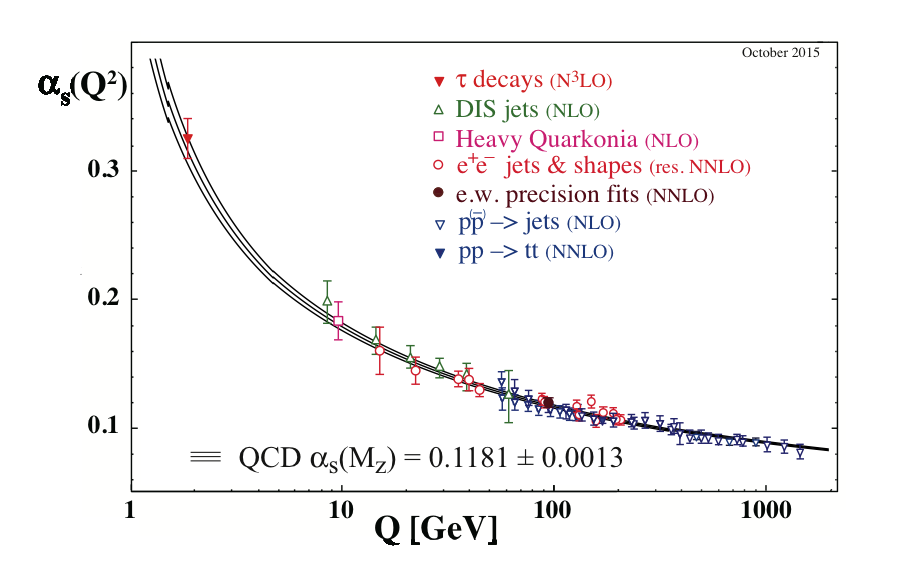
\includegraphics[width=10cm]{chap1/figure/alphas.eps}
  \caption{Summary of measurements of $\alpha_{s}$ as a function of the Q. The respective degree of QCD perturbation theory used in the extraction of $\alpha_{s}$ is indicated in brackets (NLO: next-to-leading order, NNLO: next-to-next-to leading order,  NNLO: NNLO matched with resumed next-to-leading logs, $\rm{N^{3}LO}$:next-to-NNLO)~\cite{bib_pdg}.}
  \label{fig_1_alphas}
\end{figure}

\section{Quark Gluon Plasma (QGP)}
Due to the asymptotic freedom, the coupling of QCD is estimated to become weak at high temperature. %~\cite{bib_alphatemp}.
Therefore it is anticipated that the confinement may be broken in high temperature or high density matters and the phase transition to a deconfined state called quark-gluon plasma (QGP) occurs. 
It is thought that the phase transition to QGP in heavy ion collisions at the Large Hadron Collider (LHC) described in the next section is not a first order phase transition but a crossover where there is not a clear separation of phases but the thermodynamic properties change rapidly around the critical temperature $T_{c}$. 
Figure~\ref{fig_1_lattice} shows the results of the (2+1) lattice calculation on the pressure (3p/$T^{4}$), energy density($\epsilon/T^{4}$), and entropy density ($3s/4T^{3}$) as a function of temperature when the chemical potential $\mu$ is zero\cite{bib_hotqcdlattice}.
According to this calculation, $T_{c}$ is expected 154 $\pm$ 9 MeV. 
Below $T_{c}$, the calculated results with the lattice QCD shows the reasonable agreement to the  hadron resonance gas model (HRG) which assumes all hadrons or hadron resonance states contribute to the thermodynamics as non-interacting particles.
Above $T_{c}$, the estimations of HRG lie along the lower edge of the lattice predictions and show the discrepancies from the lattice calculation as the temperature rises. 
%The results of the lattice calculation doesn't show the flat shape but an asymptotic growth to the Stefan-Boltzmann limit at high temperature. 
The results of the lattice calculation doesn't show the flat shape and underestimates compared to the Stefan-Boltzmann limit. 
It implies the interaction of gluons and quarks in the QGP might not be so weak coupled as to be approximated by the ideal gas.
\begin{figure}[!h]
	 \centering
	 \includegraphics[width=10cm]{chap1/figure/hotqcdlattice.png}
  	\caption{ Calculated result of lattice QCD on the energy density, entropy density, and pressure as a function of temperature $T$~\cite{bib_hotqcdlattice}.}
 	 \label{fig_1_lattice}
\end{figure}

%The lattice calculation predict the critical temperature ($T_{c}$) of the phase transition to QGP is 150-200 MeV. 
%Figure~\ref{fig_1_lattice} shows the calculated result of the entropy density $s/T^{3}$ as a function of temperature $T$~\cite{bib_slattice}.  
%The entropy increases close to the Steffen-Boltzmann limit rapidly around 200 MeV due to the increase of the degree of freedom.
%The increase of degree of freedom is attributed by the creation of deconfiend state composed of quarks and gluons. 
%Figure~\ref{fig_1_lattice} shows the results of the (2+1) lattice calculation on the pressure (3p/$T^{4}$), energy density($\epsilon/T^{4}$), and entropy density ($3s/4T^{3}$) as a function of temperature.
%This model take into account two light quark flavor with the same mass and one heavy flavor tuned to match the $\eta_{s\bar{s}}$ mass. 
%In the ideal gas limit, the system obeys Steffen-Boltzmann low and these values become constant. 
%The yellow band in Fig.~\ref{fig_1_lattice} shows the crossover region around the critical temperature 145 $<$ $T$ $<$ 164 MeV.
%Below 150 MeV, the results show the agreement to the hadron resonance gas approximation. 
%The discrepancy between two approximation is shown above 170 MeV. 
%They are not saturated at higher temperature but the energy density and the entropy density increase rapidly around $T_{c}$ due to the increase of the degree of freedom by the transition from the hadronic matter to the partonic matter.
%\begin{figure}[!h]
 % \centering
%  \includegraphics[width=8cm]{chap1/figure/lattice.png}
%  \includegraphics[width=10cm]{chap1/figure/latticeentropy.png}
%  \caption{ Calculated result of lattice QCD on the entropy density ($s/T^{3}$) as a function of temperature $T$~\cite{bib_slattice}.}
%  \label{fig_1_lattice}
%\end{figure}
%The lattice calculation of QCD predicts that the phase transition occurs around the critical temperature $T_{c}\sim$ 150-200 MeV. 
%Figure~\ref{} shows the calculated result of the entropy density as a function of temperature. 
%The entropy density increases  at $T\sim$ 200 MeV due to the increase of the degree of freedom, which imply the existence of the de-confined state. 


\section{Relativistic Energy Heavy Ion Collisions}
Relativistic heavy ion collisions are thought as the unique tool to create the QGP in the laboratory.
For example, the initial energy density of Pb-Pb collisions at LHC calculated by the Bjorken formula is $\epsilon_{0}\sim$ 20 GeV/$\rm{fm}^{3}$. 
%$A$ is the transverse are and $c\tau_{0}$ is longitudinal length of the considered initial 
%$\tau_{0}$ is assumed 0.08 fm.
It is much higher than the expected QGP threshold $\epsilon_{c}$ ($\sim$ 1 GeV/$\rm{fm}^{3}$).
The temperature is expected to reach up to 4 $T_{c}$.
Therefore it is believed that QGP is created in relativistic heavy ion collisions. 

The first experiment of the relativistic heavy ion collisions is performed at Bevalac in Lawrence Berkeley in the middle of 1970’s.
It is a Fixed-target experiment with the energy per nucleon of 2 A GeV.  
In 1980's, the experiments at the Alternating Gradient Synchrotron (AGS) in Brookhaven National Laboratory (BNL) and Super Proton Synchrotron (SPS) in European Organization for Nuclear Research (CERN) started with the beam energy per nucleon of $\sim$ 14A GeV and $\sim$ 160A GeV, respectively. 
The Relativistic Heavy Ion Collider (RHIC) in BNL is the first collider for the relativistic heavy ion collisions. 
The Large Hadron Collider (LHC) in CERN provides heavy ion collisions since 2010.  

Figure~\ref{fig_1_hic} shows the schematic view of the space-time evolution of heavy ion collisions~\cite{bib_spacetime}. 
It is necessary to understand the space-time evolution of heavy-ion collisions to study the formation of the QGP.
\begin{figure}[!h]
  \centering
  \includegraphics[width=12cm]{chap1/figure/hic.png}
  \caption{Space and Time evolution in relativistic heavy ion collisions. The z-axis express the beam direction. $\tau_{0}$ is the formation time of QGP. $T_{c}$, $T_{ch}$ ,and $T_{fo}$ denote critical temperature, chemical freezeout temperature, and kinematical freezeout temperature, respectively~\cite{bib_spacetime}.}
  \label{fig_1_hic}
\end{figure}
The space-time evolution of heavy ion collisions can be separated into the initial stage before collisions, pre-equilibrium stage, equilibrium stage (QGP) and expansion of the QGP, hadronic gas phase, chemical freezeout, and kinematical freezeout.
It is assumed that the space-time evolution is dependent on only the proper time $\tau=\sqrt{t^{2}-z^{2}}$ at high energy limit. 
\begin{description}
\item[Initial Stage] \mbox{}\\
When the nuclei collide at $\tau=$0, a large number of nucleon-nucleon collisions occur in the overlap region of incident nuclei. % and huge amount of energy is deposited in a small volume. 
It is non-trivial that heavy-ion collisions can be described by the superposition of nucleon-nucleon collisions due to the existence of normal nuclear effects as described in Chapter 2.
%This initial nucleus-nucleus collisions cannot is not exactly same as the superposition of the nucleon-nucleon collisions because of nuclear matter effects described in Chapter~\ref{chap_phys}.
The system is not thermalized at this points.

\item[Pre-equilibrium stage] \mbox{} \\
After initial collisions, a large amount of color flux tubes are generated between passing nuclei along the beam axis. 
This state is called as "Glasma".
Due to their instabilities, they decay into partons and the system reaches the local equilibrium at the formation time $\tau = \tau_{0}$. 
If the temperature is above the $T_{c}$ at $\tau=\tau_{0}$, QGP is formed. 
%%$\tau_{0}$ is expected very short within 1 fm/$c$.
The exact $\tau_{0}$ value is still unknown but it is estimated to be at least shorter than 1 fm/$c$~\cite{bib_flow}.


\item[Equilibrium stage (QGP) and expansion of the QGP] \mbox{} \\
Once the system becomes thermalized, the expansion of the system can be described by the relativistic hydrodynamics. 
%During the collective expansion of the system, the temperature drops and if it crosses the $T_{c}$, hadrons are generated 
The system cools down and if the temperature is below $T_{c}$, the hadrons start to be created and the system is dominated by hadrons. 

\item[Hadron gas phase] \mbox{} \\
As temperature of hadron gas decrease and when the temperature cross the chemical freezeout temperature $T_{ch}$, the relative particle ratio of hadrons are fixed although generated hadrons interact each other. 
At the kinetic freezeout temperature $T_{fo}$, the momentum distribution of hadrons is fixed and hadrons are emitted from the matter.  
\end{description}
%RHIC and LHC provides many signs of the QGP formation such as $J/\psi$ suppression and large anisotropic flow\cite{bib_jpsiaarhic}. 
%However, in order to extract QGP signal from the experimental data, whole understanding of the space-time evolution of the heavy ion collision is needed. 
The comparison between the experimental results and hydrodynamic calculation indicates that the system expands collectively with small shear viscosity to entropy density ratio ($\eta /s$) close to the lower bound 1/4$\pi$~\cite{bib_flow}. 
It implies that partons in the QGP interact strongly and the mean free path is sufficiently short compared to the system size. 


\section{Objective and Organization of Thesis}
$J/\psi$ has been considered as one of the golden probes to discuss the formation of the QGP.
As is described in Chapter 2, attraction between $c$ and $\bar{c}$ quarks is reduced by Color Debye screening in QGP and thus $J/\psi$ is not formed in the QGP.
In addition to the color screening effect in the QGP, normal nuclear matter effects such as the gluon shadowing play a role to modify the $J/\psi$ production in heavy-ion collisions. 
Understanding of the normal nuclear matter effects is mandatory for the understanding of the QGP effects to the $J/\psi$ production in heavy-ion collisions.
In this thesis, $J/\psi$ production in p-Pb collisions at the LHC is measured and normal nuclear effects to the $J/\psi$ production is described.

The organization of this thesis is as follows.  
In Chapter~\ref{chap_phys}, the physics background related to this thesis is summarized. 
In Chapter~\ref{chap_setup}, the LHC complex and the detector setup of the ALICE experiment is described. 
In Chapter~\ref{chap_ana}, the analysis of $J/\psi\rightarrow e^{+}e^{-}$ in p-Pb collisions at $\sqrt{s_{NN}}=$5.02 TeV is explained. 
In Chapter~\ref{chap_dis}, experimental results and their interpretation are discussed. 
The conclusion of this thesis is summarized in Chapter~\ref{chap_con}

\section{Major Contribution}
As one of the members in ALICE collaboration, the author carried out data taking of the ALICE experiment. 
In addition, the major contributions of the author are following. 
\begin{description}
  \item{-} Installation, commissioning, and operation of the Transition Radiation Detector (TRD).
  %\item{-} The feasibility and conceptual design study of the new scheme of the TRD pretrigger. 
  \item{-} Study of the trigger efficiency of the electron triggers with TRD in p-Pb collisions.
  \item{-} Dielectron analysis in p-Pb collisions described in this thesis.
\end{description}




\clearpage
%\setcounter{page}{1}
%\pagenumbering{arabic}

%% Chap-2 Physics Overview 

\chapter{Physics Background}
\label{chap_phys}

\section{$J/\psi$ production process}
$J/\psi$ was discovered in $p$+Be$\rightarrow$$e^{+}e^{-}X$ at AGS and $e^{+}e^{-}$ annihilation at SPEAR in Stanford Linear Accelerator Center (SLAC) in 1974~\cite{bib_jpsifirst1,bib_jpsifirst2}.
$J/\psi$ is a resonance state of $c\bar{c}$ and $J/\psi$ mass is 3096.9 MeV/$c^{2}$ slightly higher than the charm quark pair mass. 
$J/\psi$ has spin=1 without the orbital angler momentum.   

Production of $J/\psi$ can be classified into two processes, where the first process is the creation of $c\bar{c}$ and the second one is to form $J/\psi$ from $c\bar{c}$ pairs.
Since the mass of charm quarks is expected large enough compared to $\Lambda_{QCD}\sim$ 200 MeV, $c\bar{c}$ production can be described by the pertubative QCD calculation. 

\begin{figure}[!h]
  \centering
  \includegraphics[width=12cm]{chap2/figure/ccbar_diagram.png}
  \caption{Feynman diagrams of $c\bar{c}$ production. From left to right, they express gluon fusion, gluon splitting, and flavor excitation, respectively. }
  \label{fig_2_jpsidiagram}
\end{figure}

\begin{figure}[!h]
  \centering
  \includegraphics[width=8cm]{chap2/figure/production/ccbar.png}
  \caption{
    Total cross section of $c\bar{c}$ in pp collisions as a function of $\sqrt{s}$.  
    The contribution from pair creation, flavor excitation, and gluon splitting are shown separately~\cite{bib_ccbar}.
  }  
  \label{fig_2_charmxsection}
\end{figure}
Figure~\ref{fig_2_jpsidiagram} shows the Feynman diagrams of the main $c\bar{c}$ production at LHC energies~\cite{bib_ccbar}. 
The leading order of $c\bar{c}$ production is gluon fusion.
In this process, gluons from each nucleus interact and produce $c\bar{c}$. 
The next-leading order process is the gluon splitting, which scattered gluons split into $c\bar{c}$ pairs.
Another next-leading order process is flavor excitation, where a off-shell quarks produced by the virtual gluon splitting is scattered with a gluon in the other nucleus. 
Figure~\ref{fig_2_charmxsection} shows the calculated cross section of $c\bar{c}$ production and the contribution of each process in pp collisions as a function of the collision energy~\cite{bib_ccbar}. 

Several models have been developed to describe $J/\psi$ formation from $c\bar{c}$ pairs such as the color singlet model (CSM), color evaporation model (CEM), and Non-Relativistic QCD (NRQCD)~\cite{bib_csm1,bib_csm2,bib_cem1,bib_cem2}. 
However, for the moment, no model describes $J/\psi$ production and polarization simultaneously. 

%\subsubsection{Color Singlet Model (CSM)}
%The color singlet model (CSM) is assumed that a specific qaurkonium state can be formed if the charm quark anti-charm quark pairs created color singlet state with the same angler momentum quantum number as $J/\psi$. 
%In this model, hard gluon emission is needed to conserve C-parity. 

%In the leading order gluon fusion process, $J/\psi$ production whose spin number is 1 is suppressed compared to other quarkonia with spin 0 or 2 because gluons have spin 1.

%\subsubsection{color Evaporation Model (CEM)}
%In this model, the probability of $J/\psi$ formation is independent the color of $c\bar{c}$ pairs. 
%The color of $c\bar{c}$ is assumed to be neutralized by the interaction with collision induced color field. 

%\subsection{Non-Relativistic QCD (NRQCD)}
%The charmonium can be produced in a color singlet or color octet.
%the spin can be singlet or triplet and it can also have orbital angular momentum.

%\subsection{Feed Down $J/\psi$}
%CMS


\section{$J/\psi$ production in Relativistic Heavy Ion Collisions}
\label{sec_2_summary}
Compared to pp collisions, $J/\psi$ undergoes the following effects in heavy ion collisions. 
\begin{description}
  \item[Color screening]\mbox{} \\
	$J/\psi$ is not formed in QGP since attraction between charm and anti-charm quarks are screened in QGP as described in Section.~\ref{sec_2_screening}
  \item[Regeneration in QGP]\mbox{} \\
		Since the number of $c\bar{c}$ at the RHIC and LHC energies are large in heavy ion collisions, $J/\psi$ can be formed in the QGP or phase boundary from uncorrelated $c\bar{c}$ (each of pairs is produced in different nucleon-nucleon collisions.)
  \item [Modification of gluon PDF in nuclei]
	It is known as the gluon yield in nuclei is smaller than those in free proton scaled by the atomic number. 
	This is called  as the gluon shadowing. Since gluon parton distribution function (PDF) in nuclei is different from gluon PDF in free proton, simple A scaling of $J/\psi$ production from pp collisions to heavy ion collisions is not preserved.
  \item [Cronin effect]
	It is known	the momentum spectra in p-$A$ collisions become harder compared with pp collisions. 
	This is called as Cronin effect. 
	The harder shape of the transverse momentum $p_{\rm{T}}$ is expected due to the multiple scattering of incident partons in the nucleus. 
   \item [Break up and energy loss in nuclei]
%  \item [Nuclear absorption]
	$J/\psi$ or pre-resonance $c\bar{c}$ state are destructed by the collisions with spectator nucleons, which leads to the suppression of the $J/\psi$ production. 
	This depends on the relative time scale of $c\bar{c}$ of $J/\psi$ formation and crossing time of two colliding nuclei. 
	The medium induced radiative parton energy loss is expected  and depends on their formation time. 
	If the formation time of gluon emission is larger than the nuclear mean free path, this is expected coherent process. 
\end{description}
Color screening is explained in Section.~\ref{sec_2_screening}.
$J/\psi$ regeneration is described in Section.~\ref{sec_2_reco}.
The normal nuclear matter effects are summarized in Section.~\ref{sec_2_normal}.

\section{Color Screening in QGP and suppression of $J/\psi$}
\label{sec_2_screening}
Matsui and Satz proposed the suppression of $J/\psi$ production as one of the strong evidence of the QGP formation\cite{bib_matsui}. 
The mechanism is based on the Debye screening observed in the electromagnetic plasma. 
At zero temperature, the QCD potential between the quark and anti-quark is expressed by, 
\begin{equation}
V_{QCD}(r) = -\frac{4}{3}\frac{\alpha_{s}(r)}{r}+\sigma r
\label{eq_2_jpsiv}
\end{equation}
where $r$ is the distance between the quark and anti-quark and $\sigma$ is the QCD string tension. 
$\alpha_{s}$ is the gauge coupling constant of QCD described in Section~\ref{sec_1_qcd}. 

Figure~\ref{fig_2_freeenergy} shows the free energy of color singlet quark anti-quark pairs(F(r, T)) calculated by (2+1) lattice QCD~\cite{bib_jpsimodel}.  
The asymptotic value (F($\infty$, T)) corresponding to the energy needed to separate the quark anti-quark pair decrease with increasing temperature. 
\begin{figure}[!h]
  \centering
  \includegraphics[width=10cm]{chap2/figure/Suppression/FreeEnergy.png}
  \caption{Color singlet quark-antiquark free energy as a function of quark separation calculated in (2+1) lattice QCD at different temperature~\cite{bib_jpsimodel}.}
  \label{fig_2_freeenergy}
\end{figure}
%If the $\lambda_{D}$ becomes smaller than the hadronic radius, quark-antiquark pairs cannot interact with each other and become unbound. 


As the temperature increases, many free colored partons are generated and occupy the vacuum. 
The potential of the quark anti-quark pairs is modified from coulomb like potential to Yukawa potential, 
\begin{equation}
  V_{QCD}(r) = -\frac{4}{3}\frac{\alpha_{s}}{r}e^{-\frac{r}{\lambda_{D}(T)}}
\end{equation}
where $\lambda_{D}(T)$ is the debye length of the color screening. 
Qualitatively $\lambda_{D}(T)$ becomes smaller as temperature increases. 
According to lattice calculation, the second term of Eq.~\ref{eq_2_jpsiv} becomes small as temperature increases as following dependence~\cite{bib_tension}, 
\begin{equation}
  \sigma/\sigma_{0} = \sqrt{1-\frac{T}{T_{c}}}
\end{equation}
where $\sigma_{0}$ is the string tension at $T$$=$0.
At deconfined phase, second term in Eq.~\ref{eq_2_jpsiv} should be vanished or negligible small. 

Lattice calculations and potential models have been adopted to expect the dissociation temperature of each quarkonium. 
Due to the different binding energy, dissociation of quarkonium occurs sequentially towards high temperature. 
Table~\ref{table_2_melt} shows the summary of dissociation temperature $T_{d}$ in unit of $T_{c}$ for each quarkonium calculated by a potential model calculation~\cite{bib_melt}.

\begin{table}[!h]
  \centering
  \begin{tabular}{ccccccccc} \\ \hline
    State   & $J/\psi$  & $\chi_{c}(1P)$  & $\psi (2S)$ & $\Upsilon (1S)$ & $\chi _{b}(1P)$ & $\Upsilon (2S)$  & $\chi_{b}(2P)$  & $\Upsilon (3S)$ \\ \hline
    $T_{d}/T_{c}$ & 2.1 & 1.16 & 1.12 & $\geq 4.0$ & 1.76 & 1.60 & 1.19 & 1.17 \\ \hline
  \end{tabular}
  \caption{Dissociation temperature in unit of $T_{c}$ calculated using a potential model\cite{bib_melt}.  }
  \label{table_2_melt}
\end{table}

\section{$J/\psi$ Regeneration}
\label{sec_2_reco}
%The enhancement of baryon/meson ratio $\sim$ 1 is observed at in the intermediate $p_{T}\sim$ 3 GeV/c at RHIC\cite{bib_baryonmesonphenix}. 
%This cannot be described via fragmentation process but it can be described by the coalescence of neighboring quarks. 
%If the phase space is fulfilled by the quarks, the coalescence happens and generated hadrons carry the momentum of mother quarks.
\begin{figure}[!h]
  \centering
  \includegraphics[width=10cm]{chap2/figure/reco/jpsirege_schematics.png}
  \caption{
  	Schematics of $J/\psi$ regeneration in heavy ion collisions at RHIC and LHC~\cite{bib_regenature}.
	}
  \label{fig_2_recosche}
\end{figure}

The expected number of $c\bar{c}$ quarks created in heavy-ion collisions at the LHC, RHIC and SPS is about 60, 10, 0.2 as shown in Table~\ref{table_2_ncchic}, respectively.
\begin{table}
	\centering
	\begin{tabular}{cccc} \hline
	Experiment      &  SPS &  RHIC  & LHC  \\ \hline
	$N_{cc}$/$N_{ev}$ & 0.2   & 10 & 60 \\ \hline
	$dN_{ch}/d\eta$  & 450   &  650& 1500 \\ \hline	
	\end{tabular}
	\caption{Expected the number of $c\bar{c}$ and charged particles in central heavy ion collision at SPS, RHIC, and LHC. }
	\label{table_2_ncchic}
\end{table}
The yield of charmonium from regeneration depends on the ratio of the number of light quarks and charm quarks. 
The estimated number of regenerated $J/\psi$ is scaled by ($N_{coll}^{2}/N_{part}$).
%The number of $c\bar{c}$ pair production in nucleus-nucleus depends on the number of binary collisions ($N_{coll}$).
%On the other hand, light quark hadron yields are approximately scaled by the number of participants in the overlap region of colliding nuclei. 
%In the glauber calculation, $N_{coll}$ grows rapidly compared to the $N_{part}$ as the centrality of collisions increases. 
%Therefore the enhancement is more significant at central heavy ion collisions than peripheral collisions.  
Production of $c\bar{c}$ as a function of impact parameter (collision centrality) and the production of light hadrons 
scale with the number of binary collisions ($N_{coll}$) and the latter with the number of participants ($N_{part}$), respectively. 
Participants are defined as the nucleons which exist in the overlap area of colliding nuclei. 
The detail of the collision geometry of high energy nucleus-nucleus collisions is summarized in Appendix~\ref{app_a_glauber}.
Since $N_{coll}$ grows faster than $N_{part}$ as a function of centrality, regeneration of $J/\psi$ is more pronounced in more central collisions. 
The regeneration of $J/\psi$ is direct evidence of the formation of deconfied matter. 
At the LHC, where abundant $c\bar{c}$ are created, $J/\psi$ is possibly formed by the regeneration process from uncorrelated $c\bar{c}$ pairs, where $c$ and $\bar{c}$ are created in different nucleon-nucleon collisions since charm quarks are expected to be thermalized in QGP. 

Figure~\ref{fig_2_reco} shows the numerical calculation of $dN_{J/\psi}/dy$ as a function of $N_{part}$~\cite{bib_yellowpaper}.
The rapid increase with centrality shows due to the quadratic dependence of the number of $c\bar{c}$. 
%Figure~\ref{fig_2_reco} shows the transport model calculation in Pb-Pb collision at LHC at forward rapidity~\cite{bib_transport}. 
%The transport mode considers all both of QGP effects and normal nuclear matter effects. 
%According to this model calculation,  the contribution of $J/\psi$ regeneration is dominant below $p_{\rm{T}}~ <$ 4 GeV/$c$.
\begin{figure}[!h]
  \centering
  \includegraphics[width=10cm]{chap2/figure/reco/recoestimate.png}
  \caption{
	Calculation of regeneration model for $J/\psi$ production as a function of $N_{part}$ at LHC in three $c\bar{c}$ multiplicities~\cite{bib_yellowpaper}. 
	}
  \label{fig_2_reco}
\end{figure}

\section{Normal Nuclear Matter Effects in Relativistic Heavy Ion Collisions}
\label{sec_2_normal}

\subsection{Modification of Parton Distribution Function inside Nuclei}
\label{sec_2_pdf}
The cross section of the hard process between nucleon A and nucleon B is factorized as, 
\begin{equation}
  \sigma_{AB} =  \Sigma_{a, b} \int{dx_{1}}\int{dx_{2}} f^{A}(x_{1})f^{B}(x_{2})\sigma(a_{1}+b_{2})
\end{equation}
where $f^{A}$ and $f^{B}$ are the  parton distribution function (PDF). 
$\sigma(a_{1}+b_{2})$ is the cross section of partonic subprocess between the partons in A and B.
$x$ is a longitudinal momentum fraction of partons. 
In 2$\rightarrow$1 process, the relation of $x$,  rapidity, and energy is expressed by 
\begin{equation}
  x_{1, 2} = \frac{m_{T}}{\sqrt{s}}e^{\pm y}
\end{equation}
In 2$\rightarrow$2 process, the relation of x,  rapidity, and energy is expressed by 
\begin{equation}
%  x_{1, 2} = \frac{m_{T}}{\sqrt{s}}e^{\pm y}
  x_{1} = \frac{m_{T}}{\sqrt{s}}(e^{y_{1}}+e^{y_{2}}),  \\
 ~~~  x_{2} = \frac{m_{T}}{\sqrt{s}}(e^{-y_{1}}+e^{-y_{2}}) \\
\end{equation}
where $m_{T}$ is the transverse mass $m_{T}=\sqrt{m^{2}+p_{T}^{2}}$ and $\sqrt{s}$ is the collision energy per nucleon-nucleon collision in the center-of-mass system.
%In order to understand the experimental data,  the determination of PDF is crucial. 
%The useful way to determine the PDF is the Deep Inelastic Scattering (DIS)
PDF is mainly obtained from the results of deep inelastic scattering (DIS) and the calculated cross section using perturbative QCD as a function of $x$ and momentum transfer $Q^{2}$~\cite{bib_dis}. 
\begin{figure}[!h]
  \centering
  \includegraphics[width=10cm]{chap2/figure/CNM/hera.png}
  \caption{Parton distribution function measured via e-p scattering in H1 and ZEUS at HERA ~\cite{bib_hera}.}
  \label{fig_2_protonpdf}
\end{figure}
Figure~\ref{fig_2_protonpdf} shows the measured parton distribution function in protons via e-p scattering in H1 and ZEUS at HERA~\cite{bib_hera}.
They observed the rapid growth of the gluon PDF toward small $x$. 
This multiple gluon production at small $x$ is caused by long life time of the energy fluctuation and described by the BFKL equation ~\cite{bib_bfkl}. 
When the gluon density is not too high, gluons don't interact with each other and the linear growth remains. 
%%and the growth of gluon is expressed $\sim x^{-\lambda}$ with $\lambda$$\sim$0.3 by the linear BFKL equation~\cite{bib_bfkl}.
The life time of the gluon radiation with small fraction $x$ and transverse momentum transfer $k_{T}$ is, 
\begin{equation}
	\tau  \sim  \frac{1}{\Delta E} \sim \frac{2xp}{k_{T}}
\end{equation}
where $p$ is the mother parton momentum. 
Therefore this fluctuation has long life time at high energy limit and emitted gluon can generate gluons by $g\rightarrow gg$ with the probability of gluon emission$\sim~\alpha_{s}ln(1/x)$. 
Incoherent gluon emissions from gluons created in the previous steps can also occur and gluon density rapidly increase. 
In high energy pp or nucleus-nucleus collisions, scatterings of these small $x$ partons mainly occur. 

European Muon Collaboration (EMC) group observed the modification of nuclear parton distribution function (nPDF) compared to PDF in the free proton in $\mu$-Fe scattering in 1982 as shown in Fig.~\ref{fig_2_stfunc}~\cite{bib_emc}. 
The modification of the nPDF from the free proton is evaluated as the ratio of the structure function. 
They discovered the clear modification of the nucler modification factors for heavy ions. 
The right panel of Fig.~\ref{fig_2_stfunc} shows the ratio of the structure function in heavy nuclei and carbon. 
The suppression of $F^{A}_{2}/F^{C}_{2}$ is seen toward smaller $x$. 
%\begin{figure}[!h]
%  \centering
%  \includegraphics[width=8cm]{chap2/figure/CNM/emc.png}
%  \caption{The ratio of the nucleon structure functions F measured iron and deuterium as a function of $x$ measured by EMC collaboration~\cite{bib_emc}.}
%  \label{fig_2_emc}
%\end{figure}
%\begin{figure}[!h]
%  \centering
%  \includegraphics[width=8cm]{chap2/figure/CNM/stfunc.png}
%  \caption{The ratio of the nucleon structure functions F measured iron and deuterium as a function of $x$ measured by EMC collaboration~\cite{bib_emc}.}
%  \label{fig_2_emc}
%\end{figure}
\begin{figure}[!h]
  \begin{minipage}{0.5\hsize}
    \begin{center}
      \includegraphics[width=8cm]{chap2/figure/CNM/emc.png}
    \end{center}
  \end{minipage}
  \begin{minipage}{0.5\hsize}
    \begin{center}
      \includegraphics[width=8cm]{chap2/figure/CNM/stfunc.png}
    \end{center}
  \end{minipage}
  \caption{
    The ratio of the nucleon structure functions F measured iron and deuterium as a function of $x$ measured by EMC collaboration~\cite{bib_emc}.
  }
  \label{fig_2_stfunc}
\end{figure}

%For the explanation of the A-A collisions, the modification of nPDF have to understand precisely. 
%In this calculation, the nuclear modification factor defined as following, 
The nuclear modification factor of gluon PDF is introduced as follows:
\begin{equation}
  R^{A}_{i}(x, Q^{2}) = \frac{f^{A}_{i}(x, Q^{2})}{Af^{free}_{i}(x, Q^{2})}
\end{equation}
where $A$ is the mass number of nuclei, $f^{free}_{i}$ is the parton distribution function in the free proton.  
As physical explanation of gluon shadowing, multiple parton scattering with the nucleus is mainly discussed. 
However, there is not any theory to describe all experimental data. 

Figure~\ref{fig_2_pdf} show the comparison of model calculation of the gluon nuclear modification factor inside Pb at $Q^{2}=$10 $\rm{GeV^{2}}$.
In Fig.~\ref{fig_2_pdf}, the region $x$ $<$ $10^{-2}$ is called as shadowing region where the nuclear modification factor is below 1. 
The region $10^{-2} < x < 0.3$ is called anti-shadowing region/ %where merged gluons due to the shadowing effect contribute with larger $x$. 
The region above 0.3 is called as EMC region. 
\begin{figure}[!h]
  \centering
  \includegraphics[width=10cm]{chap2/figure/CNM/gluonPDF.png}
  \caption{Comparison of the model calculation of the gluon nuclear modification factor inside Pb as a function of $x$ at $Q^{2}=$10 $\rm{GeV^{2}}$~\cite{bib_pdf}. The red and blue solid squares show the $x$ coverages of the mid-rapidity $J/\psi$ measurements in ALICE at LHC ($|\eta |~ <$ 0.9) and PHENIX at RHIC ($|\eta |~<$  0.35), respectively.}
  \label{fig_2_pdf}
\end{figure}
Figure~\ref{fig_2_xcover} shows the $x$ coverage of each experiment in heavy ion collisions~\cite{bib_aprv1}. 
$c\bar{c}$ production at LHC corresponds to the order of $x\sim$ $10^{-4}-10^{-3}$~\cite{bib_aprv1,bib_aprv2}.
Therefore at the LHC energy, the gluon shadowing becomes relevant at mid-rapidity. 
\begin{figure}[!h]
  \centering
  \includegraphics[width=10cm]{chap2/figure/experimentaldata/xcoverage.png}
  \caption{$x$ and coverage of each experiment. The y-axis express transverse mass of the scattering processes~\cite{bib_aprv1}.  }
  \label{fig_2_xcover}
\end{figure}

Further small $x$ and small $Q^{2}$ region, gluon saturation is expected to occur~\cite{bib_saturation}. 
As described above in this section, gluon PDF rapidly increases at small $x$ by gluon splitting ($g\rightarrow gg$). 
However, as gluon density increases, gluon fusion process ($gg\rightarrow g$) also becomes relevant and then the gluon density becomes highly saturated. 
Gluon saturation is expected to occur when the transverse momentum transfer is below the saturation scale $Q_{s}^{2}$.
The transverse gluon density $\rho$ is expressed by the number of gluons $xG(x, Q^{2})\propto Ax^{-\lambda(Q^{2})}$ divided by the transverse area $\pi R_{A}^{2}$.
$R_{A}$ is the atomic radius with atomic mass number $A$. 
The cross section of gluon fusion is expressed by $\sigma_{gg\rightarrow g}\sim \alpha_{s}/Q^{2}$.
Gluon saturation is expected to become relevant when the probability of $\rho \sigma_{gg\rightarrow g}\sim$1~\cite{bib_saturation}. 
Therefore the saturation scale $Q_{s}$ is proportional to $A^{1/3}x^{-\lambda}$ with $\lambda \sim$ 0.3~\cite{bib_geoscale,bib_saturationscale}.

Gluon saturation is treated in the Color-Glass Condensate (CGC) framework~\cite{bib_cgc}.
CGC is an effective field theory which divides the system into large $x$ classical color field and associated small $x$ quantum fields. 
Valence partons with large $x$ act as static random color sources. 
The dynamics of the system is determined by the large $x$ valence partons. 
Small $x$ gluons are considered as classical gauge fields induced by the valence partons and this situation obeys the Yang-Mills equation. 



\subsection{Cronin Effect and $k_{T}$ broadening}
It is known that the particle yield at the moderate transverse momentum enhance in p-A collisions compared to pp collisions~\cite{bib_cronin}.
This is referred as the Cronin effect. 
It is believed to be due to the momentum broadening caused by the multiple rescattering of the partons in the nucleon inside the nucleus.  
The mean squared transverse momentum $\langle p_{\rm{T}}^{2}\rangle$ depends on the production point
\begin{equation}
  \langle p_{\rm{T}}^{2}\rangle_{pA}(\vm{b}, z) =  \langle k_{T}^{2} \rangle_{pp} + \langle p_{\rm{T}}^{2}\rangle \sigma_{gN} \int dz\rho_{A}(\vm{b}, z)
\end{equation}
Cronin effects can be approximated by the path length, 
\begin{equation}
  \langle k_{T}^{2} \rangle_{pA} =   \langle k_{T}^{2} \rangle_{pp} +  a_{gN}L%\langle\frac{2\mu^{2}L}{\lambda} \rangle
  \label{eq_2_cronin}
\end{equation}
%where $L$ is path length and $a_{gN}$ is expressed as $\frac{2\mu ^{2}}{\lambda}$. 
%where A is the mass number of incident nucleus, L is the path length which corresponds to the Lorentz-contracted longitudinal size of the nucleus, and
%$\mu$ is the the amount of the mean momentum transfer in the parton-nucleon scattering. 
%$\lambda$ is the mean free path of the parton in side the nucleus. 

%However the only simple multiple scattering model doesn't describe the particle production properly since the experimental results show the dependence on the particle species, in particular protons. 
%Figure~\ref{fig_2_chargerppb} shows the measured nuclear modification factor for pion, kaon, protons in p-Pb collision~\cite{bib_chargerppb}. 
%Proton shows the stronger enhancement around 4 GeV/c than other light mesons.
%Equation~\ref{eq_2_cronin} doesn't include any variables related to the produced particle spiceries since it only estimate the kinematics modification of parton in the nucleus but it doesn't describe the mechanism of hadron production. 
%Therefore additional nuclear matter effects have to be considered in hadronization.

%To describe the data, some theories try to understand this baryon enhancement by regeneration model~\cite{bib_starreco}. 
%They are supported by the fact that other baryons like $\Lambda$ and $\Xi$ also show the stronger enhancement compared to mesons in central p-A collisions~\cite{bib_alicebaryon,_bib_aliceomega}. 
%Figure~\ref{fig_2_baryonratio} shows the baryon/meson ratio as a function of $p_{T}$ in p-Pb collisions at $\sqrt{s_{NN}}=$5.02 TeV and Pb-Pb collisions at $\sqrt{s_{NN}}=$2.76 TeV. 
%Both of proton and $\Lambda$ shows the enhancements above $p_{T}=$2 in central p-Pb collisions. 
%It is qualitatively consistent of the regeneration picture. 
%This trend is also similar to the effect of radial flow in the created matters in central p-Pb collisions. 

%\begin{figure}[!h]
%  \centering
%  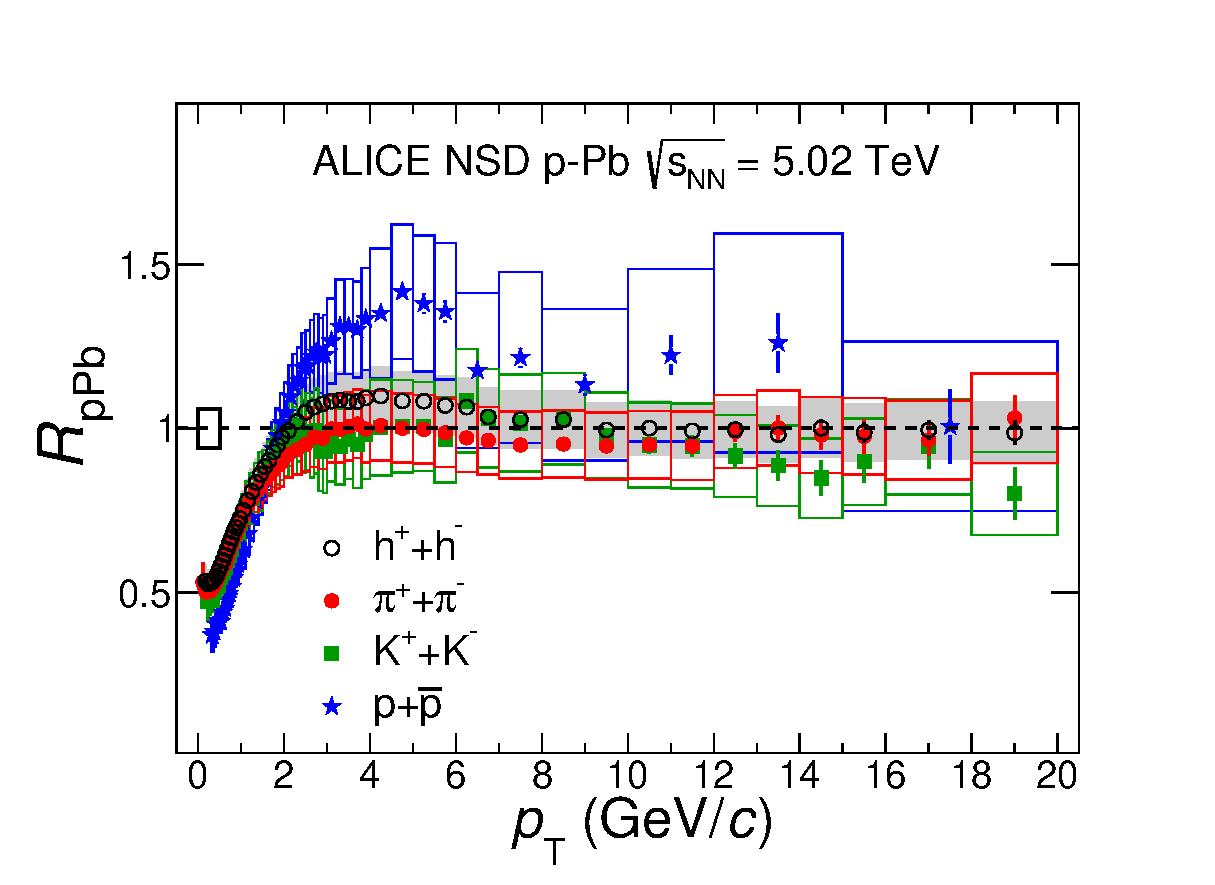
\includegraphics[width=10cm]{chap2/figure/Cronin/ChargeRpPb_ALICE.eps}
%  \caption{Inclusive $R_{pPb}$ of charged particles, $\pi$, K, $p$, $\Lambda$ at $\sqrt{s_{NN}}=$5.02 TeV~\cite{bib_chargerppb}.}
%  \label{fig_2_chargerppb}
%\end{figure}

%\begin{figure}[!h]
%  \begin{minipage}{0.5\hsize}
 %   \begin{center}
 %     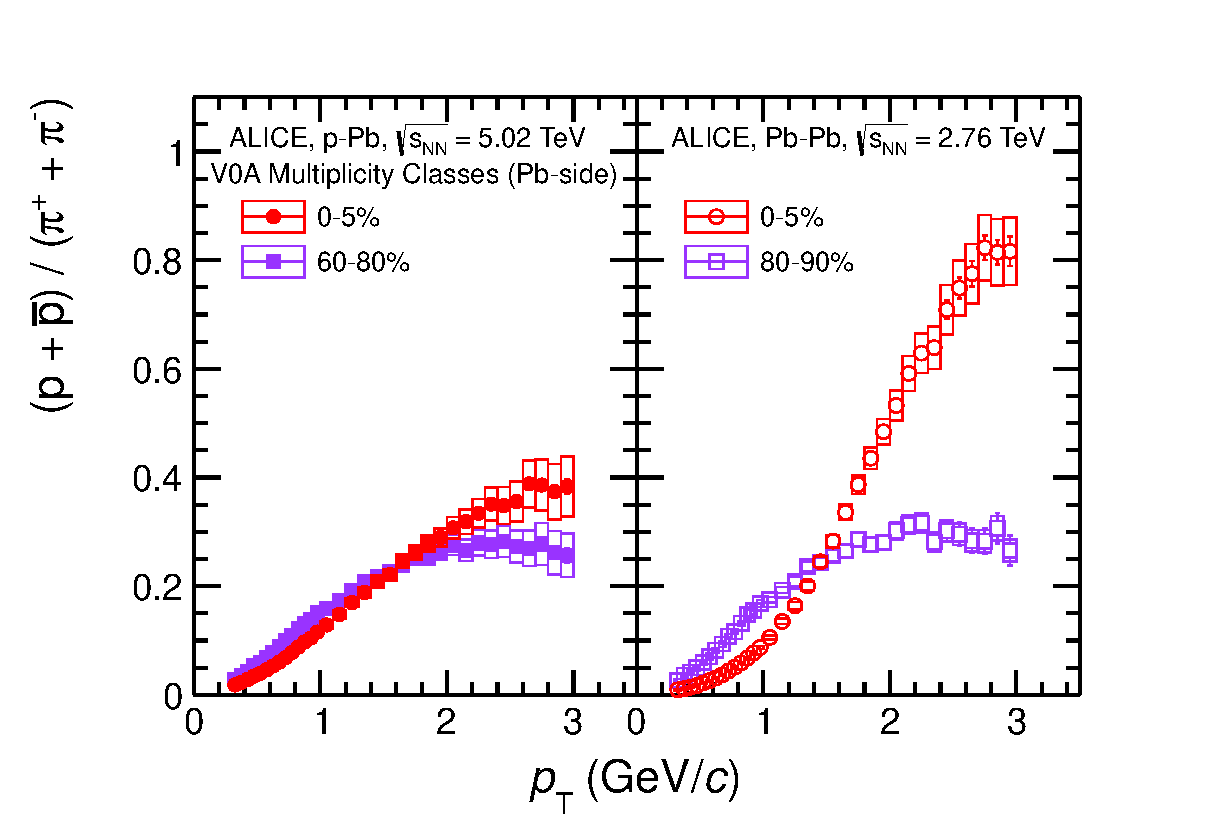
\includegraphics[width=8cm]{chap2/figure/Cronin/ProtonPionRatio_pPb.eps}
 %   \end{center}
 % \end{minipage}
 % \begin{minipage}{0.5\hsize}
 %   \begin{center}
 %     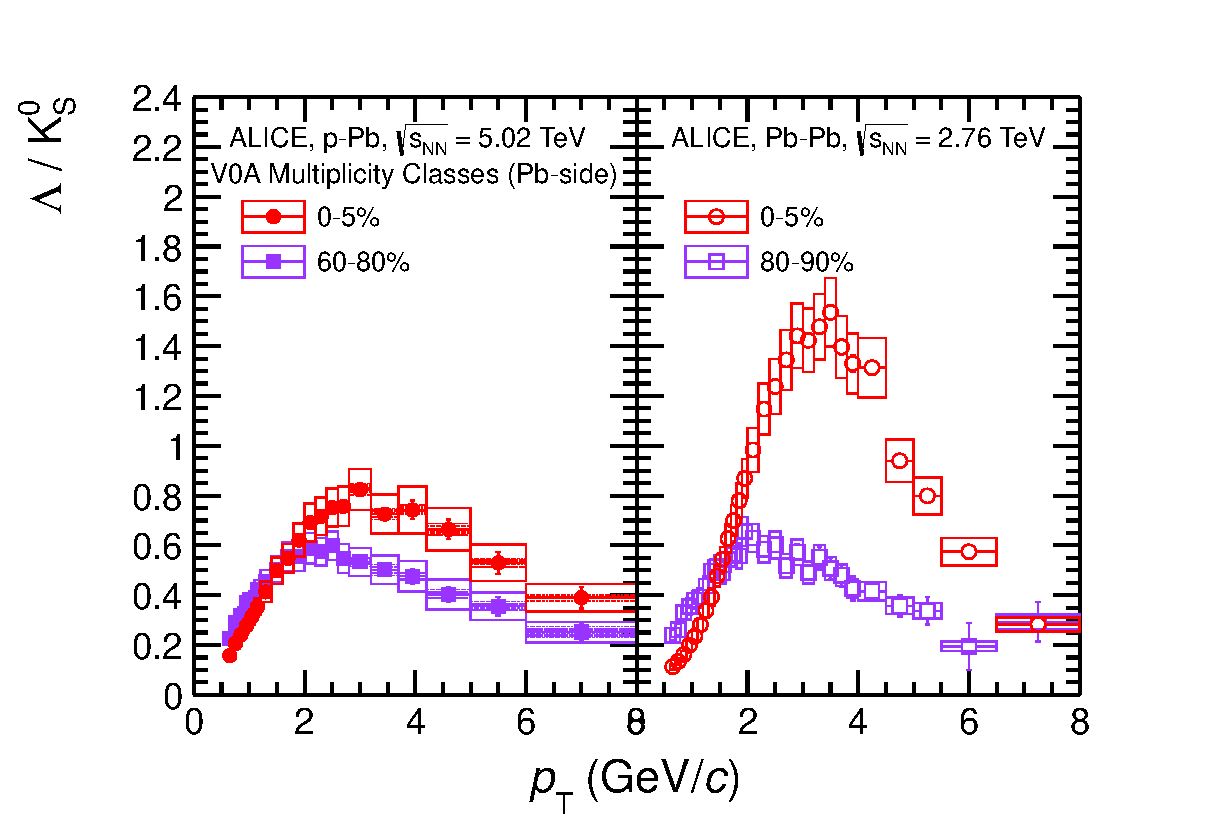
\includegraphics[width=8cm]{chap2/figure/Cronin/LambdaK0sRatio_pPb.eps}
 %   \end{center}
 % \end{minipage}
 % \caption{
 %   $p/\pi$ (Left) and $\Lambda$/$k^{0}_{s}$ (Right) ratio in p-Pb collisions at $\sqrt{s_{NN}}=$5.02 TeV~\cite{bib_alicebaryon}. 
 % }
 % \label{fig_2_baryonratio}
%\end{figure}




\subsection{Partonic Energy Loss inside the nucleus}
\label{sec_2_eloss}
Another initial state effect in heavy ion collisions is the initial state energy loss~\cite{bib_paeloss}. 
In the nuclear medium with the typical size $\sim L$, the medium induced radiative parton energy loss is expected due to the multiple interaction in the nucleus. 
%The average medium-induced radiative loss scaling as the quarkonium energy can be $\Delta E \sim E$.
%which corresponds to the time the scattered partons finish the radiative energy loss 
If the formation time of gluon radiation is shorter than the mean free path, the Cronin-like interaction mainly occurs and the radiation spectrum is similar to o the Bethe-Heitler spectrum, 
\begin{equation}
	\omega\frac{dI}{d\omega} = \frac{N_{c}\alpha_{s}}{\pi}\{  ln(1+\frac{\Delta q_{\rm{T}}^{2}E^{2}}{M_{\rm{T}}^{2} \omega^{2} }) -ln(1+\frac{\Lambda_{QCD}E^{2}}{M_{\rm{T}}^{2}\omega^{2}})    \}
\end{equation}
 where $E$ and $M_{\rm{T}}$ are the energy and transverse mass of the partons. 
 $\Delta q_{\rm{T}}$ is momentum transfer and $\Delta q_{\rm{T}}^{2}\sim\hat{q}L$ due to the momentum broadening in p-A collisions. 
$\hat{q}$ is called the transport coefficient.
In the limit of $\Lambda_{QCD} ^{2} \ll \Delta q_{\rm{T}}^{2} \ll M_{\rm{T}}^{2}$, the scaling of average energy loss $\Delta E \propto E$ is derived~\cite{bib_deltaescale}.       

When the formation time is longer than the mean free path, the coherent energy loss known as the Landau-Pomeranchuk-Migdal (LPM) effect occurs. 
In QED, this effect suppress medium induced bremsstrahlung radiation compared to the Bethe-Heitler process due to the interference between the next scatterings. 
The similar mechanism is expected in case of QCD process and the average energy loss is denoted by  $\Delta E_{\rm{LPM}} \propto \alpha_{s} \hat{q} L^{2}$.
This process can be expected in other nuclear matter effects like gluon shadowing. 

Furthermore, if the formation time is larger than path length $L$, the process is fully coherent and all scattering centers act as a source of radiation the coherent energy loss expressed by
\begin{equation}
	\Delta E \propto \alpha_{s}N_{c}\frac{\sqrt{\hat{q}L}}{M_{T}}E  ~ \gg \Delta E_{\rm{LPM}}
\end{equation}


\begin{figure}[!h]
    \begin{center}
      \includegraphics[width=12cm]{chap2/figure/eloss/eloss_arelo.png}
    \end{center}
  \caption{
  	Schematic of view of quarkonium hadroproduction in the nucleus rest frame~\cite{bib_jpsipaeloss}. 
  }
  \label{fig_2_jpsipaeloss}
\end{figure}

In case of $J/\psi$ production, the color nutralization time of the color octet state ($\tau_{octet}$) is expected larger than the perturbative time scale ($\tau_{hard}\sim 1/M$). 
Figure~\ref{fig_2_jpsipaeloss} shows the quarkonium hadroproduction in the nucleus rest frame~\cite{bib_jpsipaeloss}. 
In the nucleus mass frame, quarkonium hadroproduction by $gg\rightarrow Q\bar{Q}$ looks like small angle scattering of an color charge. 
The hadronization time ($t_{\psi} \gtrsim t_{octet} = \tau_{octet}(E/M)$) is expected long enough and hadronization happens outside of the nucleus.  
In this situation, the medium induced coherent spectrum arises from the interference between the gluon emission in the initial and final states.
The cross section of $J/\psi$ production in p-A collisions can be written by, 
\begin{equation}
	\frac{1}{A}\frac{d\sigma^{J/\psi}_{\rm{p}A}}{dE}(E, \sqrt{s})  = \int^{E}_{0}d\epsilon P (\epsilon ) \frac{d\sigma^{J/\psi}_{pp}}{dE}(E +\epsilon , \sqrt{s})
\end{equation}
where $P (\epsilon )$ is quenching weight related to the induced gluon spectrum and it includes the transport coefficient $\hat{q}$.
Figure~\ref{fig_2_paeloss} shows the initial energy loss calculation in p-Pb collisions at $\sqrt{s_{NN}}=$5 TeV by F.~Arleo $et$ $al$~\cite{bib_jpsipaeloss}. 
The transport coefficient $\hat{q}$ is taken by 
\begin{equation}
	\hat{q} (x) = \frac{4\pi^{2}\alpha_{s}N_{c}}{N_{c}^{2}-1}\rho xG(x) \sim q_{0}(\frac{10^{-2}}{x})^{0.3}
\end{equation}
$x$ dependence is considered from the HERA data described in Section~\ref{sec_2_pdf}. 
$q_{0}$ is the only free parameter in their calculation and and $q_{0} = 0.075 \rm{GeV}^{2}/$fm is obtained from the fit to E866 p-W collision data~\cite{bib_e866}.   
If the modification of Parton nPDF is neglected, the energy loss is expected to suppress the yield by a factor 20\%.

\begin{figure}[!h]
  %\begin{minipage}{0.5\hsize}
    %\begin{center}
  %\includegraphics[width=8cm]{chap2/figure/eloss/eloss_rhic.png}
    %\end{center}
  %\end{minipage}
  %\begin{minipage}{0.5\hsize}
    \begin{center}
      \includegraphics[width=8cm]{chap2/figure/eloss/eloss_lhc.png}
    \end{center}
  %\end{minipage}
  \caption{
    %Comparison of $J/\psi$ production between experimental data from RHIC and energy loss model calculation with various nPDF assumptions in d-Au\
% collision at $\sqrt{s_{NN}}=$200 GeV (Left) and Prediction of $J/\psi$ $R_{pPb}$ in p-Pb collision at $\sqrt{s_{NN}}=$ 5 TeV (Right)~\cite{bib_paeloss}.
    Prediction of $J/\psi$ $R_{pPb}$ in p-Pb collision at $\sqrt{s_{NN}}=$ 5 TeV by the energy loss model calculation with 4 nPDF settings~\cite{bib_paeloss}.
  }
  \label{fig_2_paeloss}
\end{figure}


\subsection{Nuclear Absorption}
$J/\psi$ produced at the initial parton scattering interacts with the nucleons in colliding nuclei and some fraction of $J/\psi$ decays into $D\bar{D}$. 
If the crossing time ($\tau_{c}$) of $c\bar{c}$ in the nuclear matter is longer than the formation time of quarkonia, quarkonia forms inside the nucleus and they interact the nucleons.
$\tau_{c}$ is calculated with, 
\begin{equation}
  \tau_{c} = \frac{L}{(\beta_{z}\gamma )}
\end{equation}
where  $\beta_{z}$ is longitudinal velocity of $c\bar{c}$. 
This effect describes the data at SPS energy well.
As Lorentz-$\gamma$ factor increases, the crossing time becomes short and quarkonium forms outside the nuclei. 
In this case, this absorption effect is negligible. 


The number of $J/\psi$ which interact and break up into $D\bar{D}$ is expressed by 
\begin{equation}
  L\rho_{0}\sigma_{abs}
\end{equation}
where $L$ is the effective path length, $\rho$ is the normal nuclear density, and $\sigma_{abs}$ is the absorption length. 
$L$ is calculated in Glauber model as following with the impact parameter\bm{b}, 
\begin{equation}
  L = \frac{1}{\rho_{0}}\frac{\int T_{A}(\bm{s})  T_{B}(\bm{b}-\bm{s}){A-1}T_{A}(\bm{s})+(B-1)T_{B}(\bm{b}-\bm{s}) d\bm{s} }
  {
    s\int T_{A}(\bm{s})T_{B}(\bm{b}-\bm{s})d\bm{s}    
  }
\end{equation}
The cross section of $J/\psi$in p-$A$ collisions is expressed as, 
\begin{equation}
	\sigma_{J/\psi , \rm{p}A} = \sigma_{J/\psi, pp}Ae^{-\rho_{0} L}\sigma_{abs}
\end{equation}

Figure~\ref{fig_2_sigmaabs} shows the measured $\sigma_{abs}$ as a function of collision energies\cite{bib_crosstime}. 
As collision energy increases, $\sigma_{abs}$ decrease due to the large $\gamma$ factor. 
\begin{figure}[!h]
  \begin{center}
    \includegraphics[width=8cm]{chap2/figure/experimentaldata/sigmaabs.png}
  \end{center}
  \caption{
    Measured $\sigma_{abs}$ at $y=0$ as a function of collision energy~\cite{bib_crosstime}. }
  \label{fig_2_sigmaabs}
\end{figure}



\section{Previous Measurements of $J/\psi$ production}
%$R_{AA}$ of $J/\psi$ 
%Figure~\ref{} shows the measurement of $J/\psi$ anisotropic flow with respective to the event plane. 
%The non-zero v2 suggest the regeneration of $J/\psi$




\subsection{SPS Results}
$J/\psi$ has been measured at the Super Proton Synchrotron (SPS) in CERN in S-U, Pb-Pb, and In-In collisions at $\sqrt{s_{NN}}~=$ 19.4, 17.3, and 17.3 GeV, respectively. 
The collision system and energy of charmonium experiments at SPS is summarized in Table.~\ref{table_2_sps}

\begin{table}
\centering 	
	\begin{tabular}{cccc} \\ \hline
	Experiment  & System                        &      $\sqrt{s_{NN}$ & Reference \\ \hline
	NA38            & p-Cu, U, W                 &   19.4                     & \cite{bib_2_na38pal1,bib_2_na38pal2,bib_2_na38pal3,bib_2_na38pal4}     \\
	~                   & p-, C, Al, Cu, W           & 29.1                     & \cite{bib_2_na38pah}    \\
	~                   & O-U, O-Cu, O-U,S-U   & 19.4                      & \cite{bib_2_na38aa1,bib_2_na38aa2,bib_2_na38aa3,bib_2_na38aa4,bib_2_na38aa5}   \\
	NA50           & p-Be, Al, Cu, Ag, W      &          27.4            & \cite{bib_2_na50pa1,bib_2_na50pa2} \\
	       ~             & Pb-Pb                           &    17.3                 & \cite{bib_2_na50aa1,bib_2_na50aa2,bib_2_na50aa3,bib_2_na50aa4,bib_2_na50aa5,bib_2_na50aa6,bib_2_na50aa7} \\ 
%	NA60           & p-Be,Al, Cu, In, W, Pb, U  & 
	NA60           &  In-In                             & 17.3                    &  \cite{bib_2_na60aa}  \\ \hline
	\end{tabular}		
	\caption{The collision system and energy of charmonium experiments at SPS.}
	\label{table_2_sps}
\end{table}

\end{table}
Figure~\ref{fig_2_ratiodrell} shows the ratio of measured yields to the Drell-Yang process as a function of path length in p-$A$ and $A$-$A$ collisions at NA38, NA50, NA51 since the yields of Drell-Yang process is scaled by the number of binary nucleon-nucleon collisions ($\langle N_{coll}\rangle$) described in Appendix.~A~\cite{bib_2_na50aa6} . 
p-$A$ results show the common trend due to the normal nuclear matter effects. 
From this dependence, the nuclear absorption cross section $\sigma_{abs}$ of $J/\psi$ was determined to be $\sigma_{abs}~=$ 4.2 $\pm$ 0.5 mb. 
%The solid curve shows the expected ratio including nuclear absorption. 
Figure~\ref{fig_2_ratiodrell} shows the ratio of measured cross section of $J/\psi$ and the expected yield from the normal nuclear matter effects as a function of path length $L$ in Pb-Pb collisions at $\sqrt{s_{NN}}~=$ 17.3 and 19.4 GeV at NA38, and NA50, respectively~\cite{bib_2_na50aa7}. 
The results show the clear suppression as $L$ increases in particular less bound state $\psi$. 
%The nucleus crossing time ($\tau_{c}\sim$ 0.3 fm/c) is compatible or larger than the charmonium formation time.
%At large path length, stronger suppression is observed than the normal nuclear matter effects. 
%\begin{figure}[!h]
%  \centering
%  \includegraphics[width=10cm]{chap2/figure/experimentaldata/sps_cnm.png}
%  \caption{The ratio of the measured $J/\psi$ yield to Drell-Yang process  as a function of path length in p-A and A-A collisions at NA38, NA50 and NA51\cite{bib_na50}.}
%  \label{fig_2_na50_1}
%\end{figure}
%\begin{figure}[!h]
%  \centering
%  \includegraphics[width=10cm]{chap2/figure/experimentaldata/Jpsi_SPS_HIC.png}
%  \caption{The ratio of the measured yield to the expected yield of $J/\psi$ and $\psi^{'}$ as a function of path length in A-A collisions at NA38, NA50 and NA51\cite{bib_na50}.}
%  \label{fig_2_na50_2}
%\end{figure}
\begin{figure}[!h]
  \begin{minipage}{0.5\hsize}
    \begin{center}
      \includegraphics[width=8cm]{chap2/figure/experimentaldata/sps_cnm.png}
    \end{center}
  \end{minipage}
  \begin{minipage}{0.5\hsize}
    \begin{center}
      \includegraphics[width=8cm]{chap2/figure/experimentaldata/Jpsi_SPS_HIC.png}
    \end{center}
  \end{minipage}
  \caption{
	The ratio of the measured $J/\psi$ yields to Drell-Yang process  as a function of path length in p-$A$ and $A$-$A$ collisions at NA38, NA50 and NA51 (Left)  and the ratio of the measured yields to the expected yields of $J/\psi$ and $\psi^{'}$ as a function of path length in A-A collisions at NA38, NA50 and NA5\cite{bib_2_na50aa6,bib_2_na50aa7}.
	}
  \label{fig_2_ratiodrell}
\end{figure}
Figure~\ref{fig_2_inin} shows the ratio of measured yield to the expected yield in In-In collisions at NA60 and Pb-Pb collisions at NA50 at $\sqrt{s_{NN}}~=$ 17.3 GeV as a function of $N_{part}$ described in Appendix A~\cite{bib_2_na60aa}. 
In high $N_{part}$ (centrality) events, significant suppression is observed in both Pb-Pb and In-In collisions above $N_{part}~>$ 80. 
\begin{figure}[!h]
  \centering
  \includegraphics[width=10cm]{chap2/figure/experimentaldata/sps_ininpbpb.png}
  \caption{The ratio of the measured yields to expected yields from the normal nuclear matter effects as a function of $N_{part}$ in Pb-Pb and In-In collisions\cite{bib_2_na60aa}. }
  \label{fig_2_inin}
\end{figure}

Figure~\ref{fig_2_spsmeanpt} shows the path length dependence of mean squared transverse momentum  $\langle p_{\rm{T}}^{2}\rangle$\cite{bib_2_na50aa4}. 
$\langle p_{\rm{T}}^{2}\rangle$ increases with mass number $A$ that is similar trend to Cronin effect. 
The results are fitted using the Cronin parametrization and $a_{gN} = $0.081 $\pm$ 0.004 and 0.078 $\pm$ 0.006 at $\sqrt{s_{NN}} = $ 17.3 and 19.4 GeV, respectively. Similar slope values are obtained. 
%Further measurements at HERAB and FNAL, it is indicated the slope of Cronin parametrization is independent of collision energy. 
\begin{figure}[!h]
  \centering
  \includegraphics[width=10cm]{chap2/figure/experimentaldata/sps_meanpt.png}
  \caption{The mean squared transverse momentum $\langle p_{\rm{T}}^{2}\rangle$ of $J/\psi$ in p-$A$ and $A$-$A$ collisions~\cite{bib_2_na50aa4}. }
  \label{fig_2_spsmeanpt}
\end{figure}

\subsection{E866 at Tevatron}
E866 at Tevatron in Felmi National Accelerator Laboratory (FNAL) has a wide Feynmann $x$ coverage at -0.1 $<$ $x_{F}$ $<$ 0.93. 
Feynmann-$x$ is defined as the longitudinal momentum transfer fraction $x_{1}$ and $x_{2}$ in the the projectile and the target, respectively, 
\begin{equation}
  x_{F}  = x_{1}-x_{2}
\end{equation}
%where $p_{L}$ is the longitudinal momentum. 
E866 evaluates the nuclear matter effects with parameter $\alpha$ defined as, 
\begin{equation}
  \sigma^{J/\psi}_{AB} = \sigma^{J/\psi}_{NN}(AB)^{\alpha}
\end{equation}
where $A$ and $B$ are the mass number of colliding nuclei. 
$\sigma^{J/\psi}_{AB}$ is the $J/\psi$ cross section in $A$-$B$ collisions and $\sigma^{J/\psi}_{NN}$ is the $J/\psi$ cross section in nucleon-nucleon collisions. 
Figure~\ref{fig_2_e866} shows the measured $\alpha$ as a function of $x_{F}$ in p-$A$ (p-Fe, p-W) collisions at $\sqrt{s_{NN}}~=$ 38.8 GeV. 
E866 observed $J/\psi$ suppression at high $x_{F}$ region in p-Fe and p-W collisions at $\sqrt{s_{NN}}~=$ 38.8 GeV, while  $\alpha $ is saturated to 0.96 $\pm$ 0.01 at low $x_{F}$. 
%At low $x_{F}$, quarkonium forms inside the nucleus. 
%One possibility to describe the suppression at high $x_{F}$ is a partonic interaction inside the nucleus since charmonium is expected to form outside the nucleus at high $x_{F}$ limit~\cite{bib_paeloss}.  
\begin{figure}
  \centering
  \includegraphics[width=8cm]{chap2/figure/experimentaldata/e866_xf.png}
  \caption{ $x_{F}$ dependence of $\lpha$ on $J/\psi$ production for three different data set (Top) and  $x_{F}$ and comparison between $J/\psi$ and $\psi$ (Bottom) at $\sqrt{s_{NN}}~ =$ 38.8 GeV~\cite{bib_e866}. }
  \label{fig_2_e866}
\end{figure}

\subsection{RHIC}
\label{rhic}
\subsubsection{d-Au Collisions}
\label{sec_2_dau}
\begin{figure}[!h]
  \begin{minipage}{0.5\hsize}
    \begin{center}
      \includegraphics[width=8cm]{chap2/figure/experimentaldata/jpsi_phenixdAu.png}
    \end{center}
  \end{minipage}
  \begin{minipage}{0.5\hsize}
    \begin{center}
      \includegraphics[width=8cm]{chap2/figure/eloss/eloss_rhic.png}
    \end{center}
  \end{minipage}
  \caption{
    $J/\psi$ production in d-Au at $\sqrt{s_{NN}}=$200 GeV/c measured by PHENIX at RHIC and model comparison with the NLO calculation with EPS09 nPDF and gluon saturation model (Left) Comparison of $J/\psi$ production between experimental data from RHIC and energy loss model calculation with various nPDF assumptions in d-Au collisions at $\sqrt{s_{NN}}=$200 GeV (Right)~\cite{bib_rhicjpsirdauvsy,bib_rhicjpsirdauvspt}. 
  }
  \label{fig_2_jpsiparhic}
\end{figure}
The left panel of Fig.~\ref{fig_2_jpsiparhic} shows the comparison of $J/\psi$ production between the measured results and the calculation based on the nuclear shadowing and the gluon saturation  at $\sqrt{s_{NN}}=$200 GeV~\cite{bib_rhicjpsirdauvsy}. 
The results show the suppression of $J/\psi$ production in whole measured  rapidity region. 
Shadowing $+$ hadron break up model describes $y$ dependence.
%However the $p_{T}$ dependence of $R_{\rm{dAu}}$. 
The right panel of Fig.~\ref{fig_2_jpsiparhic} shows the comparison of $J/\psi$ production between experimental data from RHIC and energy loss model calculation with various nPDF assumptions in d+Au collision at $\sqrt{s_{NN}}=$200 GeV~\cite{bib_jpsipaeloss}. 
The model shows the nPDF depedence in particular considering EPS09 PDF especially backward. 
It is thought the difference of strength of the anti-shadowing region ($x\sim ~10^{-1}$) as shown in Fig.~\ref{fig_2_pdf}.
Within the uncertainty of the nPDF, the energy loss model shows the reasonable agreement at mid-rapidity and forward rapidity. 
The mechanism of normal nuclear matter effects in d+Au collisions at RHIC is still  under discussion. 

\subsubsection{Heavy Ion collisions}
\begin{figure}[!h]
  \centering
  \includegraphics[width=10cm]{chap2/figure/experimentaldata/rhicjpsiaa.png}
  \caption{$N_{part}$ dependence of the nuclear modification factor of $J/\psi$ at mid-rapidity and forward rapidity (Upper) and the ratio of the nuclear modification factor of $J/\psi$ between forward rapidity and mid-rapidity~\cite{bib_rhicjpsiraa}.}
  \label{fig_2_rhicjpsiaa}
\end{figure}
Figure~\ref{fig_2_rhicjpsiaa} shows the nuclear modification factor of $J/\psi$ at mid-rapidity and forward rapidity in Au-Au collisions at $\sqrt{s_{NN}}=$200 GeV~\cite{bib_rhicjpsiraa}. 
The results show the strong suppression of $J/\psi$ in Au-Au collisions at both mid-rapidity and forward rapidity. 
The lower panel of Fig.~\ref{fig_2_rhicjpsiaa} shows the ratio of forward/mid nuclear modification factor.  
At $N_{part} > $100, the $J/\psi$ production at forward rapidity is also suppressed in Au-Au collisions. 
%It looks inconsistent with the color screening picture because the energy density at mid-rapidity is expected higher than that at forward rapidity. 
%This result may suggest the existence of $J/\psi$ regeneration at RHIC. 
As discussed in Section~\ref{sec_2_dau}, the measured $R_{AA}$ is affected by non-negligible normal nuclear matter effects.
In addition to the difference of the probing temperature,  the discrepancy of the results between mid-rapidity and forward rapidity is expected to come from the normal nuclear matter effects. 

In order to estimate the contribution of the normal nuclear matter effect in $J/\psi$ $R_{AA}$ experimentally, d-Au data is used and they assumes the $R_{AA}$ can be treated as a convolution of p-Au collisions~\cite{bib_daucorr,bib_daucorr2}. 
The rapidity dependent absorption cross section $\sigma^{J/\psi}_{abs}$ is extracted by fitting of EKS98 and nDSg shadowing parametrization as shown in the left panel of Fig.~\ref{fig_2_cnmraa}~\cite{bib_daucorr2}. 
The large global uncertainties come from the uncertainty of Glauber estimation of $N_{coll}$ in d-Au collisions. 
Since there is a significant difference between the impact parameter dependence of $R_{\rm{pAu}}$ and $R_{\rm{dAu}}$ mainly due to the smearing caused by the finite size of the deuteron, $R_{\rm{pAu}}$ is calculated using EKS98 and nDSg shadowing parametrization obtained by fitting to d-Au data~\cite{bib_shadowmodel}. 

The normal nuclear matter $R_{AA}$ is estimated by the Glauber calculation of Au-Au collisisions using the fitted absorption cross sections and the centrality dependent $R_{\rm{pAu}}$. 
For each nucleon-nucleon collisions, impact parameter $b_{1}$ and $b_{2}$ are determined with respect to each target nucleus and then $R_{\rm{pAu}}(b_{1}, y) \times R_{\rm{pAu}}(b_{2}, -y)$ is calculated and added to the accumulated $R_{AA}$. 
After processing all events, the accumulated $R_{AA}$ is divided by the number of events. 
The right panel of Fig.~\ref{fig_2_cnmraa} shows the estimated normal nuclear matter $R_{AA}$ in Au-Au collisions at $\sqrt{s_{NN}} =$ 200 GeV.
Although the absorption cross section has large global uncertainties due to the uncertainty of $N_{coll}$, it can be compensated and then negligible in the calculation of the normal nuclear matter $R_{AA}$  
The kinematic dependent difference in the absorption cross section do not affect the normal nuclear matter $R_{AA}$. 
As long as the method of fitting the d-Au data is consistent with the estimate of the normal nuclear matter $R_{AA}$ , the result should  be model independent. 

\begin{figure}[!h]
  \begin{minipage}{0.5\hsize}
    \begin{center}
      \includegraphics[width=8cm]{chap2/figure/experimentaldata/phenix_absxsection.png}
    \end{center}
  \end{minipage}
  \begin{minipage}{0.5\hsize}
    \begin{center}
      \includegraphics[width=8cm]{chap2/figure/experimentaldata/phenix_cnmraa.png}
    \end{center}
  \end{minipage}
  \caption{
  	Rapidity dependent absorption cross section in d+Au collisions at $\sqrt{s_{NN}}=$200 GeV(Left) and normal nuclear matter $R_{AA}$ in Au-Au collisions estimated from d-Au data at $\sqrt{s_{NN}}=$200 GeV with EKS98 parametrization (Right)~\cite{bib_daucorr2}. 
  }
  \label{fig_2_cnmraa}
\end{figure}

%To correct the nuclear matter effects, the survival fraction is defined as the ratio of $R_{AA}$ to the expected modification from the normal nuclear matter effects.
%The expected yield is extracted from the experimental data or realistic model calculation. 
%PHENIX corrected the normal nuclear matter effects using the measured d-Au results~\cite{bib_daucorr}.  
Figure~\ref{fig_2_saavse} shows $S_{AA}$ which is defined by $R_{AA}$ divided by the normal nuclear matter $R_{AA}$ as a function of the initial energy density $\epsilon _{0}$ and the formation time $\tau_{0}$for RHIC and SPS data~\cite{bib_rhicjpsisaa}.
\begin{figure}[!h]
  \centering
  \includegraphics[width=10cm]{chap2/figure/experimentaldata/saa.png}
  \caption{Survival fraction ($S_{AA}$) of the RHIC and SPS data as a function of $\tau_{0}  \epsilon_{0}$~\cite{bib_rhicjpsisaa}. }
  \label{fig_2_saavse}
\end{figure}
%In this case, formation time $\tau_{0}$ is taken as 1 fm/$c$ for all data. 
After consideration of the normal nuclear matter effects, the both results of forward and mid-rapidity shows the same monotonic suppression as a function of $\epsilon \tau$. 
Furthermore hydro$+$ $J/\psi$  model calculation describes the PHENIX data well the melting temperature $=$ 2$T_{c}$ as shown in the left panel of Fig.~\ref{fig_2_lhc_gunjicalc}~\cite{bib_gunjicalc}. 
The understanding and determination of the normal nuclear matter from the measured d-Au results allows this quantitative model comparison. 
However, regeneration calculation also show the reasonable agreement to the experimental results as shown in the right panel~\cite{bib_recomodel}. 
The mechanism of $J/\psi$ production in heavy ion is still under discussion and the LHC measurements play a crucial role on this problem. 
%both of RHIC and SPS data shows the same trend of the initial energy density dependence. 
%As another investigation of normal nuclear matter effects,  asymmetric Cu+Au collision. 
%Due to the difference of nPDF in Au and Cu, 
\begin{figure}[!h]
  \begin{minipage}{0.5\hsize}s
    \begin{center}
      \includegraphics[width=8cm]{chap2/figure/experimentaldata/gunjicalc.png}
    \end{center}
  \end{minipage}
  \begin{minipage}{0.5\hsize}
    \begin{center}
      \includegraphics[width=8cm]{chap2/figure/experimentaldata/pbmreco.png}
    \end{center}
  \end{minipage}
  \caption{
	Comparison of the PHENIX results and the hydrodynamic calculation including the  melting effects of quarkonium (Left) and the statistical regeneration model~\cite{bib_gunjicalc,bib_recomodel}.
   }
  \label{fig_2_lhc_gunjicalc}
\end{figure}



\subsection{LHC measurements}
Since the collision energy of LHC is higher than RHIC,  stronger suppression due to the color screening is expected. 
%The left panel of Fig.~\ref{fig_2_lhc_raavsnpart} shows the $J/\psi$ $R_{AA}$ in Pb-Pb collisions at $\sqrt{s_{NN}}~=$ 2.76 TeV at forward rapidity~\cite{bib_alicejpsiraa}. 
%The result shows less suppression compared with the RHIC results. 
\begin{figure}[!h]
	\centering
	  \includegraphics[width=15cm]{chap2/figure/experimentaldata/jpsiraa_npart.png}
 	 \caption{ $J/\psi$ $R_{AA}$ as a function of the charged particle multiplicity at mid-rapidity (Left) and forward rapidity (Right) in Pb-Pb collisions at $\sqrt{s_{NN}}~=$ 2.76 TeV and Au-Au $\sqrt{s_{NN}}~=$ 200 GeV~\cite{bib_anton}. }
  \label{fig_2_raanpart}
\end{figure}
%The right panel of Fig.~\ref{fig_2_lhc_raavsnpart} shows the $J/\psi$ $R_{AA}$ as a function of $p_{\rm{T}}$ and the comparison to the RHIC results and model calculations at mid-rapidity~\cite{bib_alicejpsiraamid}. 
Figures~\ref{fig_2_raanpart} show the measured $J/\psi$ $R_{AA}$ as a function of the charged particle multiplicity at mid-rapidity and forward rapidity at RHIC and LHC~\cite{bib_anton}.
Less suppression at LHC was observed  at both mid-rapidity and forward rapidity. 
The discrepancy of RHIC and LHC results might be related to the $J/\psi$ regeneration. 
On the other hand, the modification of the normal nuclear matter effects is different between RHIC and LHC. 
And thus the investigation of the normal nuclear matter effects at LHC is crucial to understand the energy dependence of $J/\psi$ production. 
At mid-rapidity in ALICE, the results show no multiplicity dependence. 
The high multiplicity events correspond to high initial energy density events. 
Therefore a simple color screening picture cannot explain this dependence. 
This result also the recombination picture. 

Figures~\ref{fig_2_raapt} show the measured $J/\psi$ $R_{AA}$ as a function of $p_{\rm{T}}$ at mid-rapidity and forward rapidity at RHIC and LHC~\cite{bib_alicejpsiraa,bib_alicejpsiraamid}.
At higher $p_{\rm{T}}$, $R_{AA}$ is compatible to the RHIC result. 
On the other hand, a large enhancement is observed above 4 GeV/$c$.
The $J/\psi$ regeneration picture gives a reasonable explanation to this enhancement. 
The transport model calculation shows the agreement to the ALICE result. 
This model calculation considers the all collision stages including both the color screening and $J/\psi$ regeneration. 
\begin{figure}[!h]
  \begin{minipage}{0.5\hsize}
  \begin{center}
	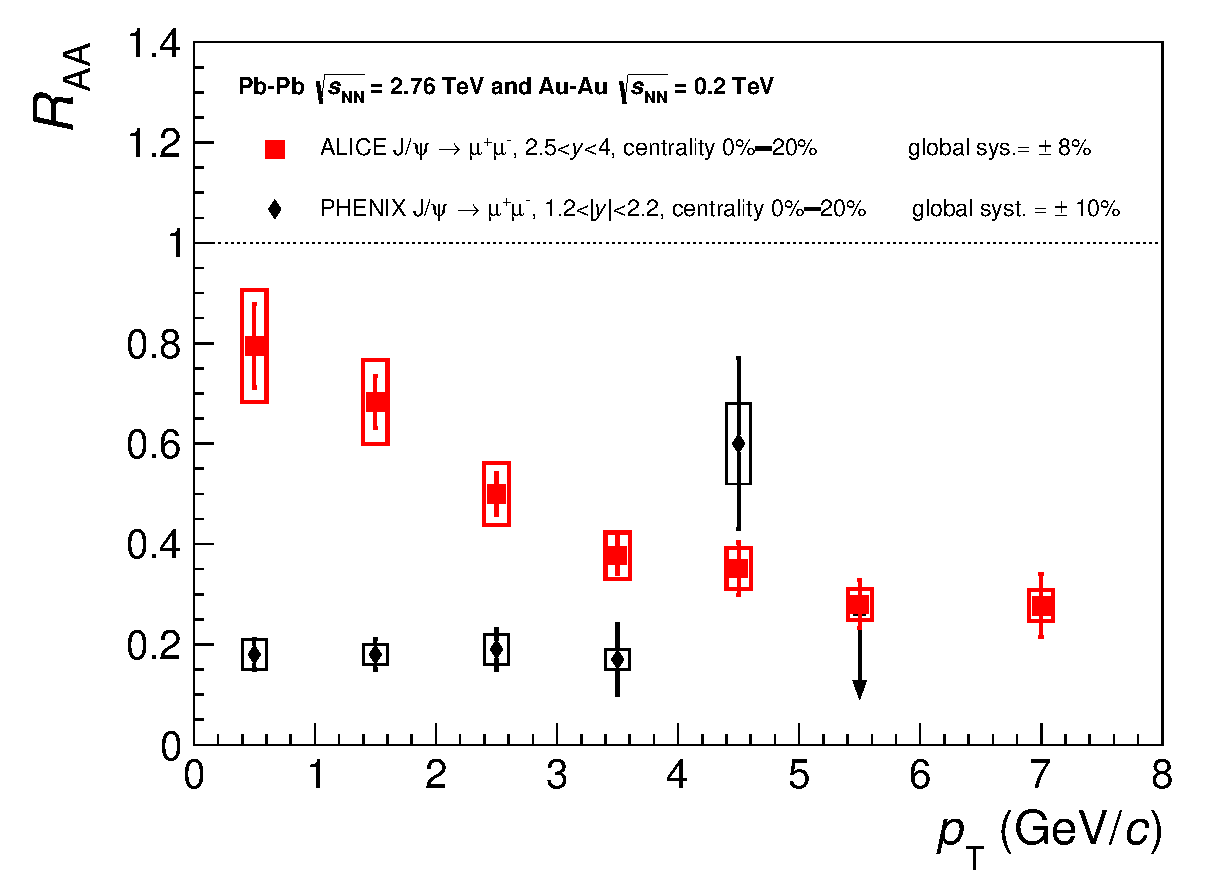
\includegraphics[width=8cm]{chap2/figure/experimentaldata/RAAPtvsModels2-4514.eps}	  
    \end{center}
  \end{minipage}
  \begin{minipage}{0.5\hsize}
   \begin{center}
      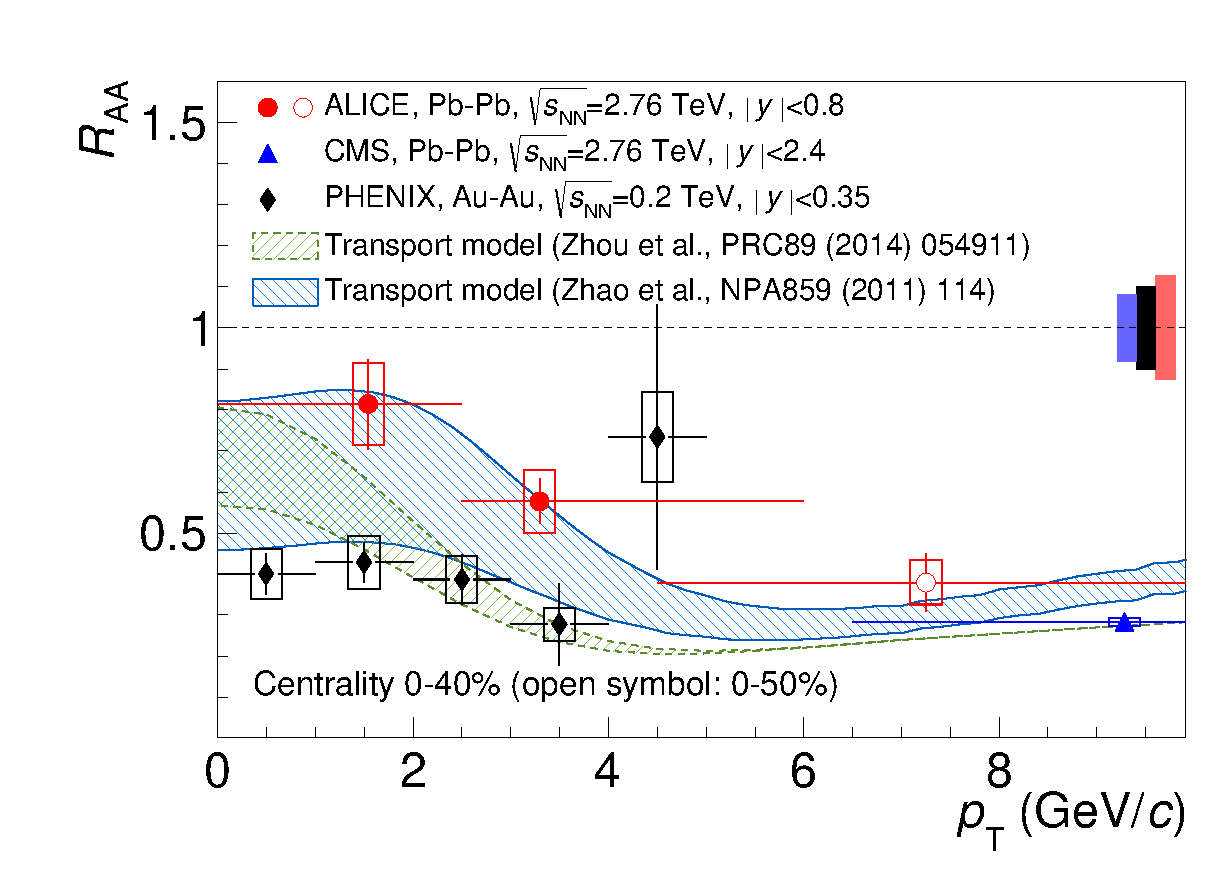
\includegraphics[width=8cm]{chap2/figure/experimentaldata/Raa-Mpt-sysBar-compPHENIX-compCMS-tcompZhou-tcompZhao-13709.eps}
    \end{center}
  \end{minipage}
  \caption{
	$J/\psi$ $R_{AA}$ as a function of the charged particle multiplicity at mid-rapidity (Left) and forward rapidity (Right) in Pb-Pb collisions at $\sqrt{s_{NN}}~=$ 2.76 TeV and Au-Au $\sqrt{s_{NN}}~=$ 200 GeV~\cite{bib_alicejpsiraa,bib_alicejpsiraamid}.
   }
  \label{fig_2_raapt}
\end{figure}

\section{Normal Nuclear Matter Effects at LHC}
Due to the large $\gamma$ factor at LHC, short crossing time of $c\bar{c}$ in the nuclear matter is expected $\sim$ $10^{-2}$ fm/$c$.
Therefore the nuclear absorption might be small or negligible at LHC energy.
The modification of nPDF is expected more crucial since more compared to the RHIC results smaller $x$ is probed at $10^{-4}$-$10^{-3}$.  
At forward or low $p_{\rm{T}}$ measurement is expected to show up the gluon saturation effect.
Cronin effect is also expected to show up in LHC measurements. 
The model calculation of the initial state energy loss in nucleus predicts relevant modifications of the $J/\psi$ production in p-Pb collisions. 

However the mechanism of normal nuclear matter is still unknown and theoretical calculations have finite uncertainties. 
%Due to the less sensitivity of Deep Inelastic Scattering, gluon nPDF still has large uncertainty at small $x$ region as described in Section.~\ref{sec_2_pdf}. 
In order to understand the normal nuclear matter effects with high precision, the experimental results of p-$A$ collisions are crucial. 
The motivation of this thesis is the investigation of normal nuclear matter effects in p-Pb collisions experimentally. 
To discuss normal nuclear matter effects, the nuclear modification factor is useful, 
\begin{equation}
  R_{\rm{pPb}} = \cfrac{Y_{\rm{pPb}}}{\langle N_{coll}\rangle Y_{\rm{pp}}}
\end{equation}
where $\langle N_{coll} \rangle$ is the average number of binary nucleon-nucleon collisions in p-Pb collisions and $Y_{\rm{pPb}}$ and $Y_{\rm{pp}}$ are yield of $J/\psi$ in p-Pb and pp collisions. 
The discrepancy from unity of $R_{\rm{pPb}}$ means the indication of nuclear matter effects. 
Normal nuclear matter effects described in this chapter are sensitive $x$, $Q$, and path length. 
Therefore the systematic measurements for the collision energy, rapidity, $p_{\rm{T}}$, and the impact parameter dependence provides  key information to understand the nuclear matter effects. 

%\section{Motivation of this study}
%The motivation of this thesis is the determine the magnitude of normal nuclear matter effects experimentally to extract the QGP signals from the result of heavy ion collisions. 
%From measured $R_{pPb}$, the extraction of $S_{AA}$ is useful for a direct comparison to $R_{AA}$. 
%The normal nuclear matter effects in heavy ion collisions is factorized by the square of the nuclear modification factor in p-Pb collisions $R_{\rm{pPb}}$ 
%\begin{equation}
%	S_{AA} ~= ~ \frac{R_{AA}}{(R_{\rm{pPb}})^{2}}
%\end{equation}
%The comparison ofof and see the initial energy dependence is important to study the thermodynamics of the system as . 


\clearpage
%\setcounter{page}{1}
%\pagenumbering{arabic}

%% Chap-3 Conceptual Design Considerations

\chapter{Experimental Setup}
\label{chap_setup}
The data analyzed in this thesis is p-Pb collisions at $\sqrt{s_{NN}}=$ 5.02 TeV in Large Hadron Collider (LHC).
LHC is a high energy hadron collider for pp, p-Pb, and Pb-Pb collisions located at CERN. 
The data was collected by the ALICE detectors in 2013 winter. 

In this chapter, the experimental set up of this thesis is described. 
Most of the parts of the detector performance is referred to the ALICE Physics Report I, II and Performance of the ALICE Experiment at the CERN LHC~\cite{bib_aprv1,bib_aprv2,bib_aprrun1}. 


\section{The Large Hadron Collider (LHC)}
\label{sec_3_LHC}
The Large Hadron Collider (LHC) is the largest particle accelerator in the world. 
The accelerator occupies the 27 km underground circular tunnel across the border between Switzerland and France which was formerly used for the Large Electron-Positron Collider (LEP). 
LHC can store and accelerate the various hadrons with 16 radio-frequency (RF) accelerating cavities and over 1600 superconducting magnets. 
The design energy of collided proton and lead is 7 TeV and 2.75 TeV/nucleon, respectively.

LHC hosts the 4 main experiments, ATLAS, CMS, LHCb, and ALICE which focus on different high energy particle and nuclear physics. 
ATLAS (A Toroidal LHC Apparatus), CMS (Compact Muon Solenoid), and ALICE (A Large Ion Collider Experiment) collected the data of the heavy ion collisions during Run1 (2009 - 2013) and contribute various progress related to the QGP physics. 
LHCb also took p-Pb collision data in 2013 and have a plan to take the heavy ion collision data from Run2 (2016-).

Figure~\ref{fig_3_lhc} shows the schematics view of the CERN accelerator complex~\cite{bib_cernaccel}. 
Protons are accelerated by a linear accelerator LINAC2. Before injected into the Proton Synchrotron (PS), the booster accelerate them to 1.4 GeV. 
They are sent PS and Super Proton Synchrotron (SPS) sequentially and accelerated to 450 GeV. 
And then they are transferred to two rings of LHC.
They go around the two rings in the opposite direction. 
Lead ions are also accelerated in similar process but there are some differences.
Lead ions are generated by heating a highly purified lead sample up to around 550.
At this stage, $Pb^{27+}$ is dominant. 
They are accelerated via LINAC3 and pass through the carbon foil which strips them to $Pb^{+54}$. 
They are also accelerated via Low Energy Ion Ring (LEIR) before injected into PS up to 72 MeV per nucleon.
PS accelerate them 5.9 GeV per nucleon and they are transferred into the foil again and fully stripped. 
The fully stripped ions are accelerated at SPS up to 177 GeV and sent to LHC rings. 
The injected protons and leads are further accelerated by LHC and finally two opposite beams of protons or heavy ions are delivered and collide at four interaction points of main experiments.
During Run1, pp at $\sqrt{s}=$ 900 GeV, 2.76 TeV, 7 TeV, and 8 TeV, p-Pb $\sqrt{s_{NN}}=$ 5.02 TeV and Pb-Pb $\sqrt{s_{NN}}=$ 2.76 GeV were provided by LHC. 
\begin{figure}[!h]
  \centering
  \includegraphics[width=12cm]{chap3/figure/LHC/CERNAcceleratorComplex.jpg}
  \caption{Schematics of CERN Accelerator Complex~\cite{bib_cernaccel}.}
  \label{fig_3_lhc}
\end{figure}


\section{Overview of the ALICE Detectors}
\label{sec_3_ALICE}
A Large Ion Collider Experiment (ALICE) is one of the major experiments in LHC dedicated heavy ion collisions. 
The all data analyzed in this thesis is collected with the ALICE detectors. 

Figure~\ref{fig_3_alicefigure} shows the schematics of ALICE detectors. 
In order to cope with high particle multiplicity in heavy ion collision events (up to $dN/d\eta \sim$ 8000) and cover a wide momentum active range with excellent particle identification, various detectors with high granularity and good PID performance in specific momentum ranges are installed in the central barrel and combined analysis for these detectors is performed. 
%The number of readout channels is enormous and the data size of one heavy collision reaches. 
%The data bandwidth is assumed. 

The determination of event characteristics is crucial to study heavy ion physics as discussed in Chapter~2.
V0, FMD, and ZDC are mainly aimed to determine the event centrality.  
The acceptance and main technology of each detector is summarized in Table~\ref{table_3_alicedet}. 
The detail of the detectors related to this thesis is described from the next section. 

\begin{figure}[!h]
  \centering
  \includegraphics[width=15cm]{chap3/figure/ALICE/ALICE_Schematics.jpg}
  \caption{Schematics of ALICE detectors~\cite{bib_aprrun1}.}
  \label{fig_3_alicefigure}
\end{figure}

\begin{table}[!htb]
  \centering
  \small
    \begin{tabular}{|r|c|c|c|c|} \hline
    Detector & $\eta$ coverage  & $\phi$ coverage & Technology & Main Purpose \\ \hline
    ITS SPD & $|\eta| < $1.4 & full & Silicon & tracking, vertexing \\
    SDD & $|\eta| < $ 0.9  & full & Silicon & tracking, low pt PID \\
    SSD & $|\eta| < $ 1.0  & full & Silicon & tracking, low pt PID \\
    TPC & $|\eta| < $ 0.9  & full & Ne/Ar drift+MWPC & tracking, PID \\
    TRD & $|\eta| < $ 0.9  & full & TR+Xe drift+MWPC & tracking, electronPID \\
    TOF & $|\eta| < $ 0.9  & full & MRPC & PID \\
    EMCAL & $|\eta| < $ 0.7 & 80  $<\phi<$ 187  & Pb+scintillator & photon, electron ID, jet \\
    V0 V0A& 2.8 $< \eta < $ 5.1 & full & scintillator & L0, Multiplicity \\
    V0 V0C& -3.1 $< \eta < $ -1.7 & full & scintillator & L0, Multiplicity \\
    T0 T0A& 4.6 $< \eta < $ 4.9 & full & quartz & Timing, Vertexing \\ 
    T0 T0C& -3.3 $< \eta < $ -3.0 & full & quartz & Timing, Vertexing \\ 
    Muon Chamber & -4.0$<\eta < $-2.5 & full &MWPC &Muon tracking \\	  
    Muon Trigger & -4.0$<\eta < $-2.5 & full &RPC &Muon trigger \\ \hline  	     
      \end{tabular}
 \caption{ Summary of acceptance and main technology for subdetectors in ALICE~\cite{bib_aprrun1}.}
  \label{table_3_alicedet}
\end{table}

In this thesis, the global coordinate system in ALICE is defined as shown Fig.~\ref{fig_3_alicecood}. 
It is a right-handed coordinate system with Z-axis. 
The Z-axis is parallel to the mean beam direction. 
The positive Z-axis is the opposite direction of the Muon arm, called 'A-side'. 
On the other hand, 'C-side' is defined as the opposite side of A-side. 
\begin{figure}[!h]
  \centering
  \includegraphics[width=10cm]{chap3/figure/ALICE/ALICE_Coordinate.png}
  \caption{Global coordinate of ALICE detectors~\cite{bib_aprv2}.}
  \label{fig_3_alicecood}
\end{figure}


\section{ALICE Global Detectors}
\label{sec_3_ALICEglobal}
\subsection{V0 Detector}
The V0 detector is a scintillation detector used for the minimum bias trigger decision and the determination of event characteristics mainly. 
V0 is formed of V0A and V0C on either side of the interaction point. 
V0A is located 340 cm away from the interaction point and covers 2.8 $< \eta < $ 5.1. 
V0C is also installed 90 cm from the interaction point and covers -3.1 $< \eta < $ -1.7.
They have 4 and 8 segments in the r and $\phi$ direction, respectively as shown in Fig.~\ref{fig_3_v0det}. 

\begin{figure}[!h]
  \centering
  \includegraphics[width=6cm]{chap3/figure/V0/CrossSection_V0.png}
  \caption{Segmentation of V0 detector~\cite{bib_aprv1}.}
  \label{fig_3_v0det}
\end{figure}

The event centrality and the event plane is estimated via measurements of the charge particle multiplicity in each segment of V0. 
Figure~\ref{fig_3_v0multi} shows the sum of V0A amplitude distribution in p-Pb collisions which is proportional to the charged particle multiplicity\cite{bib_v0multi}.
The red-line in Fig.~\ref{fig_3_v0multi} shows the result of NDB-Glauber fit~\cite{bib_ndbglauber1,bib_ndbglauber2,bib_ndbglauber3,bib_ndbglauber4}. 
The event centrality is determined by the percentile of this distribution. 
\begin{figure}[!h]
  \centering
  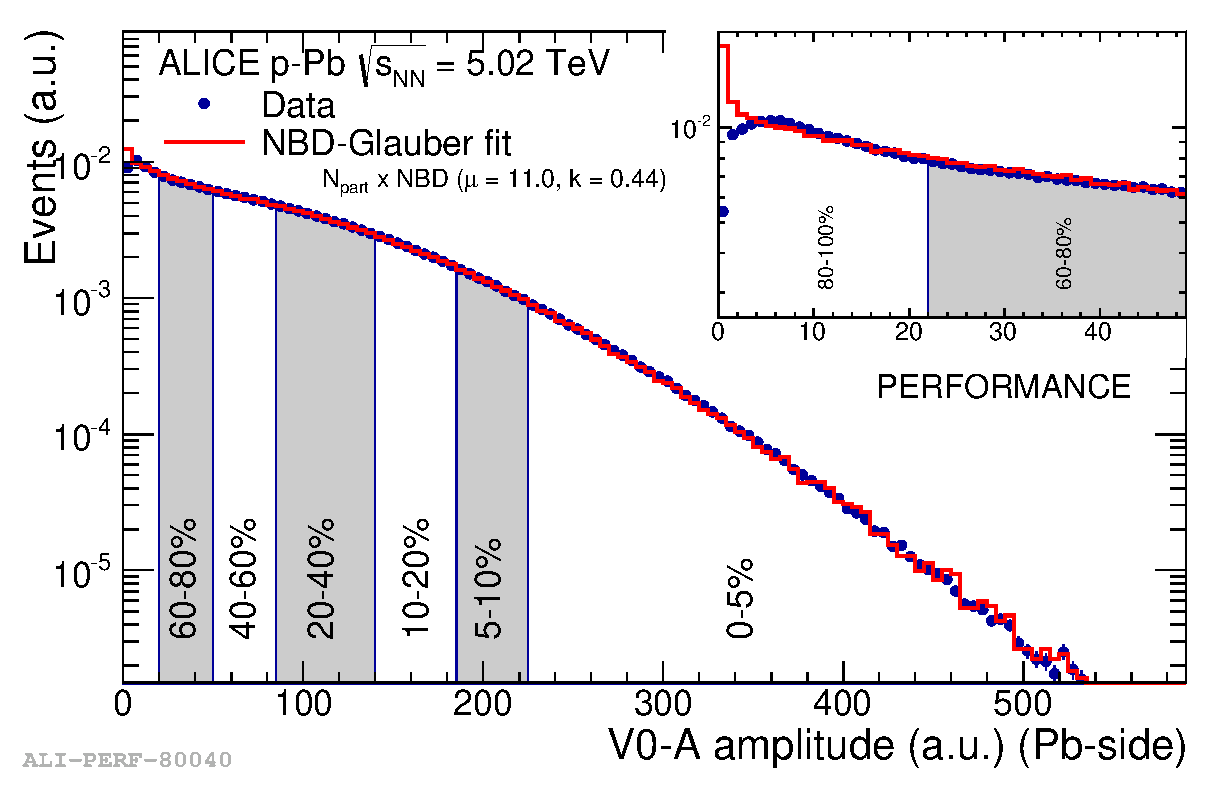
\includegraphics[width=10cm]{chap3/figure/V0/V0AMulti_pPb.eps}
  \caption{V0A multiplicity distribution in p-Pb collision at $\sqrt{s_{NN}}=$5.02 TeV (Pb-going side)~\cite{bib_v0multi}.}
  \label{fig_3_v0multi}
\end{figure}

The timing resolution of V0 is about 1 ns which enable to reject background events caused by beam-gas and beam-halo events. 


\subsection{T0 Detector}
The T0 detector is the arrays of Cherenkov counters to measure the collision time with high precision. 
The collision time is used as the reference time for TOF detector. 
The time resolution of T0 achieves 25 ps. 
T0 is also used of the determination of vertex position with a precision of about 1.5 cm. 
If the collision vertex reconstructed by T0 signal is inside the expected window, L0 trigger is issued.  
The signal from T0 also contribute to the pretrigger signal for TRD. 

\section{Detectors in ALICE Central Barrel}
\label{sec_3_ALICEcentral}
The main tracking detectors in the central barrel are ITS, TPC, and TRD. 
The strength of the solenoid magnet in the central barrel which was inherited from the former LEP experiment L3 is configurable 0.2-0.5 T in the direction of z-axis and the $p_{T}$ cut of charged particles is $p_{T}>$ 0.1 GeV/c. 
\subsection{Inner Tracking System (ITS)}
The Inner Tracking System (ITS) is the closest detector to the collision point. 
Figure~\ref{fig_3_itslayout} shows the layout of ITS. 
ITS consist of 6 layers of silicon detectors, two each of Silicon Pixel Detector (SPD), Silicon Drift Detector (SDD), Silicon Strip Detector (SSD). 
SPD is based on hybrid silicon pixels which consist of silicon detector diodes with thickness of 200 $\mu$m. 
SDD consists of a 300 $\mu$m  thick layer of homogeneous high-resistivity silicon. 
SSD is formed of double-sided silicon micro-strip sensors. 
The strip pitch is 95 $\mu$m  and the relative p-n side stereo angle is 35 mrad. 
ITS cover the full azimuthal acceptance and the pseudo-rapidity coverage of SPD and SDD is $|\eta|<$ 2.0 and $|\eta|<$ 0.9, respectively.  
The typical features of each layer detector is summarized in Table.~\ref{table_3_itsdet}. 
\begin{figure}[!h]
  \centering
  \includegraphics[width=10cm]{chap3/figure/ITS/Schematics_ITS.png}
  \caption{Schematics of ITS layout~\cite{bib_itstdr}.}
  \label{fig_3_itslayout}
\end{figure}

\begin{table}[!htb]
  \centering
  \begin{tabular}{|c|c|c|c|c|c|} \hline
    Layer & Detector Type  & Radius (cm) & Length (cm) & $\Delta$r$\phi$ ($\mu$m) & $\Delta$Z ($\mu$m) \\ \hline
    1     & SPD            & 3.9         & 28.2 & 12 & 100 \\ \hline 
    2     & SPD            & 7.6         & 28.2 & 12 & 100 \\ \hline
    3     & SDD            & 15.0        & 44.4 & 35 & 25 \\ \hline
    4     & SDD            & 23.9        & 59.6 & 35 & 25 \\ \hline
    5     & SSD            & 38.0        & 86.2 & 20 & 830 \\ \hline
    6     & SSD            & 43.0        & 97.8 & 20 & 830 \\ \hline
  \end{tabular}
  \caption{ Detector type and general features of each layer of ITS~\cite{bib_itstdr}.}
  \label{table_3_itsdet}
\end{table}

Figure~\ref{fig_3_firstpp} shows an example of ITS hits and track reconstruction in pp at $\sqrt{s_{NN}}=$ 900 GeV~\cite{bib_firstpp}. 
The main purpose of ITS is to determine the position of the primary vertex and secondary decay vertex. 
It is also useful for the precise determination of the impact parameters which enables to separate charm and bottom decay contributions by the difference of decay length. 
The offline tracking is done with combined information of ITS and TPC. 
ITS provide the reference to improve the momentum resolution of TPC. 

\begin{figure}[!h]
  \centering
  \includegraphics[width=8cm]{chap3/figure/Vertexing/ALICEfirstevent_pPb.png}
  \caption{ITS hits of first proton-proton collision at $\sqrt{s_{NN}}=$900 GeV. The navy points show the hit on ITS and the red lines show the reconstructed tracks~\cite{bib_firstpp}.  }
  \label{fig_3_firstpp}
\end{figure}


Since the readout of SDD and SSD is analog, ITS can provide the information on specific dE/dx in SDD and SSD which follow the Bethe-Bloch formula for each specie and it is used for the particle identification at relatively low momentum particles below 1 GeV/c. 

\subsection{Time Projection Chamber (TPC)}
Time Projection Chamber (TPC) is a large gaseous detector. 
TPC is used as the main tracker in the central barrel of ALICE. 
The specification of TPC is as following, 
\begin{itemize}
\item dE/dx resolution: better than 5\%. \\
\item Relative $p_{T}$ resolution: better than 1\% at $p_{T}=$1 GeV/c and 2.5\% at $p_{T}=$4 GeV/c. \\
\item Two track resolution capability capability of separating tracks with a relative momentum difference $<$ 5 MeV/c.
\end{itemize}
Figure~\ref{fig_3_tpclayout} shows the schematics of TPC.
It consists of large cylindrical gas chamber with 85 cm inner radius and 250 cm outer radius. 
The length is 500 cm along with the z-axis. 
The gas volume is 88 $\rm{m^{3}}$ and filled with $\rm{Ne/CO_{2}}$ or $\rm{Ar/CO_{2}}$.
During Run1, it was filled with $\rm{Ne/CO_{2}}$ (90\%/10\%) mixture gas.
\begin{figure}[!h]
  \centering
  \includegraphics[width=12cm]{chap3/figure/TPC/Schematics_TPC.png}
  \caption{Schematics of TPC layout~\cite{bib_tpctdr}.}
  \label{fig_3_tpclayout}
\end{figure}

The structure of the field cage is also cylindrical to maintain an uniform electric field between the Central Electrode (CE) and both end-planes (A-side and C-side).
In case of $\rm{Ne/CO_{2}}$ mixture gas, the field cage is operated at the drift field$=$400 V/cm with 100 kV at the CE. 
The maximum drift time reaches 90 $\mu$s.
The primary electrons ionized by the interaction of charge particles inside the active volume drift toward the both end-planes of A-side and C-side.
The gating grid of the readout chambers are usually closed and it is opened if TPC accepts L1 trigger signal in 6.5 $\mu$s after a collision.
It prevents from space charges in the drift region due to drifting back of positive ions generated by the multiplication of the readout chamber which cause background signals. 
The signal charges are multiplied by the Multi-Wire Proportional Chambers (MWPCs) with the gain ~7000-8000 as shown in Fig.~\ref{fig_3_tpcchamber}. 
The signals are induced in the pad-planes which have 159 readout pad rows along the perpendicular direction of the beam axis.
\begin{figure}[!h]
  \centering
  \includegraphics[width=12cm]{chap3/figure/TPC/Schematics_MWPCs.png}
  \caption{Schematics of readout chambers of TPC~\cite{bib_tpctdr}.}
  \label{fig_3_tpcchamber}
\end{figure}
The analog signals shaped with Preamplifier and Shaper (PASA) are digitized by 10-bit pipelined-ADC with 5 MHz sampling~\cite{bib_pasa}. 
They are used for the clustering and provide the 3-D position of specific energy loss by the ionization. 

\subsection{Transition Radiation Detector (TRD)}
\label{sec_3_trd}
The main purpose of the Transition Radiation Detector (TRD) is to give electron identification with good e/$\pi$ separation in wide momentum range and tracking capability of charged particles in the central barrel.
The e/$\pi$ separation reaches to 100 above 1 GeV/c. 
%Figure~\ref{fig_3_5_3} shows the picture of a TRD super module. 

TRD which surrounds TPC covers the full azimuthal acceptance with 18 super modules with the pseudo-rapidity coverage $|\eta| <$ 0.9. 
The super module is divided into 5 stacks along the $\eta$ direction. 
Each stack consists of 6 layers of MWPCs filled with $\rm{Xe/CO_{2}}$ (85\%/15\%) with the radiators (polypropylene fiber mat) for the transition radiation in front of their chambers as shown Fig.~\ref{fig_3_trdlayout}.
In total, 540 chambers(18 super modules in $\phi$ $\times$ 5 stacks in $\eta$ $\times$ 6 layers in r) are installed in principle but during Run1, 13 super modules were installed. 
The lower super modules don't contain the center stack due to the reduction of the material budget in front of PHOS detector. 
\begin{figure}[!h]
  \centering
  \includegraphics[width=8cm]{chap3/figure/TRD/CrossSection_Chamber.png}
  \caption{The corss section of the structure of TRD chamber\cite{bib_trdtdr}.}
  \label{fig_3_trdlayout}
\end{figure}

%\begin{figure}[!h]
%  \centering
%  \includegraphics[width=8cm]{chap3/figure/TRD/SuperModules.png}
%  \caption{Super module of TRD during assembly.}
%  \label{fig_3_5_3}
%\end{figure}
%\begin{figure}[!h]
%  \centering
%  \includegraphics[width=12cm]{chap3/figure/TRD/Schematics_TRDChamber.png}
%  \caption{Schematics of readout chambers of TRD.}
%  \label{fig_3_5_2}
%\end{figure}

Charged particles generated in collisions penetrate into the radiator which has 4.8 cm depth first. 
The condition of the transition radiation in the radiator is, 
\begin{equation}
  \gamma > 800
\end{equation}
At LHC energy, only electrons fulfill this condition, 
Therefore TRD can separate the electrons and pions by detecting the deposited charges of transition radiation photons.
Since Xe has a good absorption length for transition radiation photons ($E_{TR}\sim$ 10 keV) as shown in Fig.~\ref{fig_3_xe}, transition radiation photons are sufficiently absorbed just in front of the radiator. 
\begin{figure}[!h]
  \centering
  \includegraphics[width=8cm]{chap3/figure/TRD/AbsorptionLength.png}
  \caption{Absorption length for gases~\cite{bib_trdtdr}.}
  \label{fig_3_xe}
\end{figure}

The left panel of Fig.\ref{fig_3_trdschema} shows the schematics of the readout chamber. 
The readout chamber is operated with the drift field$=$700 V/cm and the drift velocity reaches 1.5 cm/$\mu$s.
In this operation, the Lorentz Angle reaches 8 rad in the magnetic field of the L3 magnet. 
The maximum drift length which corresponds to that of transition radiation photons is 3 cm. 
The signals are readout with PASA and TRAP (Tracklets Processor) chip on the Multi-Chip Module (MCM) mounted on the Readout Board (ROB). ROB is located at the back-plane of chambers.%~\cite{bib_trap}.
The operation of the subdetectors is based on the L0, L1, and L2 trigger signals generated from CTP in ALICE for the synchronization and prevention of detector busy as described in Section~\ref{sec_3_trigger}. 
However it is more complicated in case of TRD. 
For the power consumption and noise reduction, the TRAP chips are usually in the low power mode that the front-end ADC is off. 
Therefore a wake-up signal for the electronics is needed but L0 trigger has too long latency from an interaction to cope with the full signal deposited in the TRD chambers. 
\begin{figure}[!h]
 \begin{minipage}{0.5\hsize}
  \begin{center}
  \includegraphics[width=8cm]{chap3/figure/TRD/Schematics_TRDChamber.png}
  \end{center}
 \end{minipage}
 \begin{minipage}{0.5\hsize}
  \begin{center}
  \includegraphics[width=7cm]{chap3/figure/TRD/PulseHeight.png}
  \end{center}
 \end{minipage}
  \caption{Left: Schematics of the readout chamber of TRD. Left: Average pulse height as a function of the drift time for pions and electrons. The signal of transition radiation photons contribute to the latter time bins~\cite{bib_trdtdr}.}
  \label{fig_3_trdschema}
\end{figure}

The wake-up signal is issued by the pretrigger system without the latency of CTP communication.%~\cite{bib_pretrigger}.  
The pretrigger box is placed just under the central ALICE detectors to reduce transport latency (inside the L3 magnet).
It receives L0 inputs from fast detectors, V0, T0, and TOF detectors which are the same signals sent to CTP. 
Therefore in the ideal case for example neglecting detector busy, the same trigger condition is achieved. 
After decision in the pretrigger box, the wake up signal is sent to all TRD sectors and the operation of ADC start to work. 
The later L0 trigger signals from CTP are forwarded to the supermodules via the pretrigger system. 
In p-Pb collisions during Run1, the pretrigger efficiency is about 90\%. 

The sampling frequency of 10-bits ADC in TRAP is 10 MHz and the number of time bins is 22-24.
The right panel of Fig.~\ref{fig_3_trdschema} shows the pulse height for electrons and pions~\cite{bib_trdtdr}. 
The signals contain specific energy loss for each species via ionization and the contribution of transition radiation photons. 
The contribution of transition radiation photons is localized at the latter time bins since they have long drift length. 
The digital filtering for the ADC data like non-linearity, pedestal filter, gain correction, and tail cancellation is done in the MCM.


TRAP chip also has hardware preprocessor and two-stage CPUs for the cluster finding and tracklet reconstruction. 
Therefore TRD has an online tracking capability and provide rare event triggers for electrons and charged jets.
The online track reconstruction of TRD is summarized in Appendix. 
%The online track reconstruction is described in Section.\ref{sec_3_trdonline}. 
%\begin{figure}[!h]
%  \centering
%  \includegraphics[width=12cm]{chap3/figure/TRD/DataProcess_TRD.png}
%  \caption{Data processing of TRD\cite{bib_trdpaper}.}
%  \label{fig_3_5_5}
%\end{figure}

All raw data and local tracklet data for online event triggers are sent to the Global Tracking Unit (GTU). 
GTU decides to proceed further steps by receiving L0 trigger from CTP. 
And then, if L1 trigger is accepted, the data is transferred to Data Acquisition system (DAQ).

Figures~\ref{fig_3_trdepi} show the performance plots of e/$\pi$ separation using TRD~\cite{bib_aprrun1}.
1DLQ method is using inclusive charge sum for the electron likelihood calculation. 
On the other hand, 2DLQ method is based on the calculation of integrated charge sum dividing former time bins and that for the latter time bins. 
Since the signals of transition radiation localize in the latter time window, better e/$\pi$ separation can be performed compared to 1DLQ method.
%The result of Neural Network using electron and pion samples has potential .  
Figure shows the pion efficiency with 90\% electron efficiency with different methods.
The pion rejection can reach 100 at $p_{T}=$2 GeV/c. 
\begin{figure}[!h]
 \begin{minipage}{0.5\hsize}
  \begin{center}
  \includegraphics[width=7cm]{chap3/figure/TRD/TRDEleEffvsPiEff.eps}
  \end{center}
  \label{fig_3_trd_1}
 \end{minipage}
 \begin{minipage}{0.5\hsize}
  \begin{center}
  \includegraphics[width=7cm]{chap3/figure/TRD/TRDPionEffvsP_pPb.eps}
  \end{center}
 \end{minipage}
  \caption{Left Panel: Electron Efficiency vs Pion Efficiency with TRD PID in p-Pb collision at $\sqrt{s_{NN}}=$5.02 TeV. Right Panel:Pion Efficiency at the electron efficiency $=$ 90 \% with TRD PID as a function of transverse momentum in p-Pb collision at $\sqrt{s_{NN}}=$5.02 TeV~\cite{bib_aprrun1}
.
}
  \label{fig_3_trdepi}
\end{figure}


\subsection{Time-Of-Flight detector (TOF)}
Time-Of-Flight detector (TOF) is used for the particle identification of pions, kaons, protons, and electrons at $p_{T} <$ 3.0 GeV/c.
Figure~\ref{fig_3_toflayout} shows the layout of TOF. 
It is located at radius of 3.8 m and covers the full azimuthal and $|\eta| < $ 0.9 acceptance with 18 super modules in $\phi$. 
\begin{figure}[!h]
  %\begin{minipage}{0.5\hsize}
    \begin{center}
      \includegraphics[width=10cm]{chap3/figure/TOF/SuperModule_TOF.eps}
    \end{center}
  %\end{minipage}
    \caption{Schematics of Super modules of TOF and detail of one TOF module of aluminium honeycomb plane~\cite{bib_toftdr}.}
    \label{fig_3_toflayout}
\end{figure}

Figure~\ref{fig_3_tofmrpc} shows the schematics of MRPCs for TOF. 
TOF consists of an array of Multi-gap Resistive Plate Chamber (MRPCs). 
The chamber is divided into two stack on each side of the central anode. 
Each stack has five gas gaps of 250 $\mu$m to keep high and uniform electric field. 
  %\begin{minipage}{0.5\hsize}
\begin{figure}
    \begin{center}
      \includegraphics[width=8cm]{chap3/figure/TOF/TOFMRPC.eps}
    \end{center}
  %\end{minipage}
  \caption{ 
    Schematics of MRPCs for TOF~\cite{bib_toftdr}.
  }
  \label{fig_3_tofmrpc}
\end{figure}
When charged particles transverse the chambers, avalanche of electrons are produced immediately. 
The avalanche electrons are readout with pad of 2.5$\times$3.5 $cm^{2}$ arranged in 2 rows.
The time resolution of TOF itself achieves 40 ps. 
The start time of Time-Of-Flight is determined by the T0 detector.
Considering other uncertainties, the arrival time of charged particles can be measured with less than 100 ps resolution. 

Combined with momentum measurement, the relative velocity which is proportional to arrival time at TOF for each species distribute with the following relationship, 
\begin{equation}
  \beta = \frac{p}{m_{0}\gamma c}
\end{equation}

In addition, TOF also contribute to the pretrigger for TRD wake-up. 

\section{Vertexing}
\label{sec_3_vtx}
Primary vertex which is thought as the collision vertex is performed by two steps. 
First estimation of primary vertex which is thought as the collision vertex is performed by the hits on SPD detectors.
The pairs of SPD hits in each two layer which have close azimuthal angle are selected as tracklets.
Tracklets have to across the cylindrical fiducial region. 
Fiducial cuts for tracklets selection are optimized in each collision system with respect to the efficiency and background contamination.
Tracklets are selected within DCA between pair of tracklets $<$ 1 mm. 
For all tracklets, the following value is calculated,  
\begin{equation}
  d_{i} = \Sigma \frac{x_{i}-x_{0}}{\sigma_{x_{i}}}
\end{equation}
where $x_{0}$ is the expected 3-D position of the vertex, $x_{i}$ $\sigma_{x_{i}}$ is the 3-D position and the resolution of the tracklets. 
The position of the primary vertex with SPD is determined from minimum D = $\Sigma d_{i}^{2}$. 
This routine is done twice with two (loose/tight) cut setting on fiducial region and $\Delta\phi $. 
SPD is operated in the magnetic field but the effect can be negligible because of the small radius.
This vertex is used for track reconstruction. 

The final determination of primary vertex is recalculated with reconstructed tracks using ITS and TPC.  
The 3-D position of primary vertex is calculated using central between selected track pairs. 
These positions are determined as the position of the closest approach of the two tracks.  

Figure~\ref{fig_3_vtxperformance} show the finding efficiency and the position resolution of the primary vertex reconstruction with reconstructed tracks as a function of the charged particle multiplicity. 
\begin{figure}[!h]
  \begin{minipage}{0.5\hsize}
    \begin{center}
      \includegraphics[width=8cm]{chap3/figure/Vertexing/Efficiency_Vtx.png}
    \end{center}
  \end{minipage}
  \begin{minipage}{0.5\hsize}
    \begin{center}
      \includegraphics[width=8cm]{chap3/figure/Vertexing/Resolution_Vtx.png}
    \end{center}
  \end{minipage}
  \caption{ 
    Efficiency (Left) and position resolution (Right) of the primary vertex with 3-D method in case of pp collisions~\cite{bib_vtxreso}.  
  }
  \label{fig_3_vtxperformance}
\end{figure}

\section{Tracking System of Charged Particles with the ALICE Detectors}
\label{sec_3_trackrec}
\begin{figure}[!h]
  \centering
  \includegraphics[width=7cm]{chap3/figure/TrackReconstruction/Schematics_TrackingALICE.png}
  \caption{Principles of tracking for an ALICE event, showing the three successive paths allowing to build a track and refine its parameters. Numbers ranging from 1 to 10 mention the bits that are activated in case of success during the propagation of the Kalman filter at the considered stage~\cite{bib_schematrackrec}.}
  \label{fig_3_trackrec}
\end{figure}
Track reconstruction in the central barrel is performed using clusters found in each detector along the trajectory of charged particles. 
The track reconstruction follows three steps as shown Fig.~\ref{fig_3_trackrec}. 
%The start point of tracking is determined by the TPC clusters induced by ionization along the trajectory of charge particles.
The start point of tracking is determined by the most outer cluster in the TPC where the track density is relatively lower than inner detectors. 
TPC provides 159 clusters which are reconstructed from 2-dimensional information on pad-plane-time. 
Track is fitted using Kalman-Filter algorithm inward. 
The track state vector is chosen as 
\begin{equation}
  x^{T} = (y, z, C, tan\lambda, \eta)
\end{equation}
where y, z are local position in the TPC, C is coverture and $\lambda$ is dip angle between the track and padplane as shown Fig.~\ref{fig_3_tpclocalcood}. 
\begin{figure}[!h]
  \centering
  \includegraphics[width=7cm]{chap3/figure/TrackReconstruction/TPCLocalCoodinate.png}
  \caption{Local coordinate system for one sector of TPC.}
  \label{fig_3_tpclocalcood}
\end{figure}
This process is done from high momentum candidate because these tracks can be found more precisely compared to low momentum tracks. 
After propagation to the most inner ITS layer, the propagation is done again from ITS to TPC using Kalman-Filter. 
This propagation also include the hits of TRD, TOF, and EMCAL. 
Finally, the propagation called 'refit' is done from outward to ITS for the determination of the track position. 



Figure~\ref{fig_3_trackeff} shows the TPC track finding efficiency in pp and Pb-Pb collisions~\cite{bib_aprrun1}. 
There is a consistency between the reconstruction efficiency in pp and Pb-Pb collisions. 
It implies that the reconstruction efficiency is not affected by the charged particle multiplicity due to high granularity of the detectors.  
\begin{figure}[!h]
  \centering
  \includegraphics[width=10cm]{chap3/figure/TrackReconstruction/TrackEff.png}
  \caption{TPC track finding efficiency in pp and Pb-Pb collisions~\cite{bib_aprrun1}.}
  \label{fig_3_trackeff}
\end{figure}

Figure~\ref{fig_3_momreso} shows the transverse momentum resolution in p-Pb collisions~\cite{bib_aprrun1}.
The y-axis is defined as following, 
\begin{equation}
  \frac{\sigma_{p_{T}}}{p_{T}} = p_{T}\sigma_{1/p_{T}}.
\end{equation}
With ITS hits, the momentum resolution can be improve significantly. 
The impact parameter of reconstructed tracks can also be determined precisely using ITS. % that enables to separate charm and bottom contribution. 
\begin{figure}[!h]
  \centering
  \includegraphics[width=10cm]{chap3/figure/TrackReconstruction/MomReso_pPb.png}
  \caption{Inverse momentum resolution in p-Pb collisions at $\sqrt{s_{NN}}=$5.02 TeV~\cite{bib_aprrun1}.}
  \label{fig_3_momreso}
\end{figure}


\section{Particle Identification in ALICE}
\label{sec_3_pid}
ALICE uses various detectors and techniques in wide momentum range to identify particle species. 
The main technique of the particle identification is specific energy loss (dE/dx) of charged particles deposited in the detectors such as ITS, TPC and TRD.
The mean deposited energy loss in detectors can be described by the Bethe-Bloch formula.
\begin{equation}
  -\langle \frac{dE}{dx}\rangle = \frac{4\pi}{m_{e}c^{2}} \frac{nz^{2}}{\beta^{2}} ( \frac{e^{2}}{4\pi\epsilon_{0}} )^{2} [ ln( \frac{2m_{e}c^{2}\beta^{2}}{I(1-\beta^{2})} ) - \beta^{2} ]
\end{equation}
where $e$ is the elementary charge, $m_{e}$ is the electron mass, $n$ is the number density of electrons in the traget material, $z$ is the charge of the particle, and $I$ is the average ionisation potential of the target atom. 

TOF is useful to separate proton and kaon up to 4 GeV/c by measuring the flight time of particles. 
EMCAL also detects electron and photon with their deposited energy. 
%For the high $p_{T}$ particle identification, HMPID can be used. 
However they are not used in this analysis due to the limited acceptance and low reconstruction efficiency. 

\subsection{TPC PID}
The key information for the particle identification in ALICE is TPC dE/dx. 
Figure~\ref{fig_3_tpcpid} shows the deposited energy in TPC (dE/dx) as a function of reconstructed momentum in p-Pb collisions~\cite{bib_aprrun1}.
\begin{figure}[!h]
  \centering
  \includegraphics[width=10cm]{chap3/figure/PID/TPCdEdx_p_pPb.eps}
  \caption{TPC dE/dx vs reconstructed momentum in p-Pb collision at $\sqrt{s_{NN}}=$5.02 TeV~\cite{bib_aprrun1}.}
  \label{fig_3_tpcpid}
\end{figure}
Since the probability of energy loss in TPC follows the Landau distribution, the measured raw TPC signals have long tail at higher side.
In order to reduce the Landau fluctuation of TPC dE/dx for better performance of particle separation, the truncated means of all TPC clusters in the tracks are taken as the value of TPC PID.
The average fraction of truncation is about 20-30\%.  
The truncated mean of TPC dE/dx can be approximated to the gaussian and the resolution reaches up to 5\% for cosmic ray as shown in Fig.~\ref{fig_3_tpcpidreso}~\cite{bib_tpcreso}. 
%The typical PID resolution is about 5-8\%.
\begin{figure}[!h]
  \centering
  \includegraphics[width=10cm]{chap3/figure/TPC/TPCdEdx_resolution.png}
  \caption{TPC dE/dx resolution with cosmic rays as a function the number of TPC hits~\cite{bib_tpcreso}. }
  \label{fig_3_tpcpidreso}
\end{figure}

\section{Trigger System in ALICE}
\label{sec_3_trigger}
All communication on trigger information between subsystems is done via Central Trigger Processor (CTP) with TTC protocol~\cite{bib_ctp,bib_ttc}.
Figure~\ref{fig_3_ctp} shows the block diagram of CTP~\cite{bib_ctp}. 
CTP provides the trigger information and LHC timing signal (BC and Orbit) to subdetectors and also accept trigger signal from subdetectors.  

The trigger scheme in ALICE consists of 3 steps called as Level-0 (L0), Level-1 (L1), Level-2 (L2) trigger, respectively.
Level-0 trigger is mainly used for minimum bias event trigger and the initial activation of some subdetectors. 
L0 trigger inputs from fast subdetectors like V0, T0, EMCAL, and Muon detector are delivered into CTP within 900 ns after a collision. 
It is issued by the L0 processor in CTP, and then L0 accept signal is sent to subdetectors after 1.2 $\mu$s after a collision, 
If L0 is not accepted, all components become ready for the next L0 event. 

The purpose of Level-1 trigger is rare event detection. 
If each subdetector which contributes to L1 trigger receives L0 accept signal, a calculation for L1 issue is performed and L1 contribution is sent to CTP.  
It is issued after 6.5 $\mu$s from an interaction.
If L1 trigger is accepted, raw data of subsystem is transferred to the multi event buffers. 

Level-2 trigger is issued about 100 $\mu$s after the decision of L0 trigger which is determined by the drift time of TPC. 
If L2 trigger is issued, the data is transferred from the event buffers in each subdetectors to (DAQ). 

\begin{figure}[!h]
  \centering
  \includegraphics[width=10cm]{chap3/figure/Trigger/CTP.png}
  \caption{Block diagram of CTP~\cite{bib_ctp}.}
  \label{fig_3_ctp}
\end{figure}

%\section{Online Electron Triggers with TRD}
%\label{sec_3_trdonline}
%The online reconstruction of TRD are following. 
%%1. local clustering
%Cluster finding in each chamber is performed by the hardware preprocessor in TRAP chip with two dimensional ADC information of pad rows and time bins. 
%Figure~\ref{fig_3_10_localclustering} shows an example of cluster finding and tracklet reconstruction. 
%The position of clusters is calculated as the center of gravity for each time bin.
%Tracklets are reconstructed by straight line fit for clusters. 
%Tracklets contain 32-bit word information on local position in TRD, deflection, and PID. 
%The data of tracklets are then sent to GTU with 1080 optical fibers after 4.5 $\mu$s after a collision. 
%\begin{figure}[!h]
%  \centering
%  \includegraphics[width=10cm]{chap3/figure/Online/LocalClustering.png}
%  \caption{Cluster finding and tracklets reconstruction in MCM~\cite{bib_trdonline}.}
%  \label{fig_3_10_localclustering}
%\end{figure}


%Global tracking is divided into 2 parts, track matching and track reconstruction. 
%It operates in parallel on subsets of the tracklets which are compatible with a track in the x-z plane, i.e. groups of tracklets which fall into roads pointing to the nominal primary vertex. 
%These are propagated to a plane.
%Tracklets which are close enough on this plane are considered to belong to the same track. 
%The algorithm exploits a fixed read-out order of the tracklets to reduce the number of tracklet combinations which have to compared. 
%In this way, a linear scaling of the tracking time with the number of tracklets is achieved.

%Only selected tracks are reconstructed by the straight line fit as shown in Fig.~\ref{fig_3_10_globaltracking}. 
%The transverse offset from the nominal vertex position is used to estimate the transverse momentum (a $\propto$ 1/$p_{T}$).
%\begin{figure}[!h]
%  \centering
%  \includegraphics[width=12cm]{chap3/figure/Online/GrobalTracking.png}
%  \caption{Schematics of global tracking in the TRD stack with GTU.}
%  \label{fig_3_10_globaltracking}
%\end{figure}

%Figure\ref{fig_3_10_momreso} shows the online momentum resolution of TRD. 
%The typical value of the resolution is better than 10 \%.
%\begin{figure}[!h]
%  \centering
%  \includegraphics[width=10cm]{chap3/figure/Online/onlinemomreso.png}
%  \caption{Online momentum resolution of TRD.}
%  \label{fig_3_10_momreso}
%\end{figure}

%\begin{figure}[!h]
%  \begin{minipage}{0.5\hsize}
%    \begin{center}
%      \includegraphics[width=8cm]{chap3/figure/Online/LookUpTable.png}
%    \end{center}
%  \end{minipage}
%  \begin{minipage}{0.5\hsize}
%    \begin{center}
%      \includegraphics[width=8cm]{chap3/figure/Online/likelihood.png}
%    \end{center}
%  \end{minipage}
%  \caption{ 
%    Left: Lookup table for online electron identification of TRD. Right: Electron likelihood distribution for electrons and pions. 
%  }
%  \label{fig_3_10_elepid}
%\end{figure}
%The left panel of Fig.~\ref{fig_3_10_elepid} shows the lookup table for the online electron identification. 
%The look up table is generated from measured electron and pion samples. 
%The electron likelihood is calculated with 1-D deposited charge sum. 
%The PID value of online tracks is determined by the average of tracklet PID. 

%The right panel of Fig.~\ref{fig_3_10_elepid} shows the electron likelihood distribution for electrons and pions using the lookup tables. 
%TRD provide the 2 different electron triggers during Run1 p-Pb periods as show in Table.~\ref{table_3_10_trigger}. 
%Both triggers require the hit on the first layer of TRD to reduce the contribution of conversion electrons. 
%During Run1, 13 out of 18 super modules of TRD were installed. 
%\begin{table}
%  \centering
% \begin{tabular}{cccc} \hline
%   Trigger & Online $p_{T}(GeV/c)$  & PID (Electron Likelihood) & Layers \\ \hline
%   Heavy Flavor Single Electron & $\geq$3 & $\geq$0.56 & $\geq$5 \\
%    Quarkonia & $\geq$2 & $\geq$0.64 & $\geq$5 \\ \hline
%  \end{tabular}
%  \caption{Electron triggers with TRD during Run1.}
%  \label{table_3_10_trigger}
%\end{table}


\section{Run Condition and Data Set}
\label{sec_3_runcondition}
ALICE took p-Pb collision data in 2 conditions, 'p-Pb' and 'Pb-p'.
p-Pb collisions are defined as a collision traveling Pb from C-side. 
On the other hand, Pb-p collisions are defined that Pb is delivered from A-side. 
Due to the asymmetric energy of colliding protons (4 TeV) and leads (1.58 TeV), rapidity of Center-of-Mass is slightly shifted in the direction of Pb-going ($\sim 0.465$).
%The maximum manageable interaction rate of ALICE is 200 kHz and it corresponds to $10^{29}~s^{-1}\rm{cm}^{-2}$.

Table~\ref{table_3_runcondition} shows the run condition in p-Pb collisions. 
Figure\ref{fig_3_luminosity} shows the integrated luminosity of p-Pb collision during Run1~\cite{bib_aprrun1}. 
The integrated luminosity of the TRD triggered data in $p$-Pb collisions is 1.4 $\rm{nb^{-1}}$.
It corresponds to 20 times larger statistics than the current minimum bias data (0.067 $\rm{nb^{-1}}$).

\begin{figure}[!h]
  \centering
  \includegraphics[width=10cm]{chap3/figure/DataSet/IntegratedLuminosity_pPb.png}
  \caption{Integrated luminosity in p-Pb collisions at $\sqrt{s_{NN}}=$5.02 TeV collected with ALICE in 2013~\cite{bib_aprrun1}.}
  \label{fig_3_luminosity}
\end{figure}


\begin{table}
  \centering
  \begin{tabular}{c|c} \hline
    Parameters             & Value                                \\ \hline
    Proton Energy          & 4 TeV                                \\
    Pb Energy              & 1.58 TeV                             \\
    Protons per bunch      & 2 $\times ~ 10^{10}$                     \\ 
    Pb ions per bunch      & 2 $\times ~10^{8}$                      \\
    Peak Luminosity        & 1 $\times ~10^{29} ~s^{-1}\rm{cm}^{-2}$       \\
    $\beta^{*}$            & 0.8                                  \\
    Transverse width       & 150 $\rm{\mu}$m                      \\
    Longitudinal emittance  & 6 cm                                 \\
    Number of Interacting Bunch & $\leq$ 338                         \\
    Collision frequency of LHC & 112.45 kHz                       \\
    Bunch spacing & 200ns                                         \\ \hline
  \end{tabular}
  \caption{Typical beam parameters for p-Pb collision in LHC Run1.}
  \label{table_3_runcondition}
\end{table}




\clearpage
%\setcounter{page}{1}
%\pagenumbering{arabic}

%% Chap-4 Physics Performance

\chapter{Data Analysis}
\label{chap_ana}
%\section{Analysis Overview}
%\label{sec_4_overview}
The main aim of this analysis is to extract $J/\psi$ spectra at mid-rapidity region in p-Pb collisions.  
The analysis is performed using the minimum bias data of p-Pb collisions at $\sqrt{s_{NN}} =$ 5.02 TeV collected during LHC Run1 in 2013 winter.
$J/\psi$ measurements have been performed in ALICE central barrel using dielectron (electron-positron pair) decay channels. 
In this analysis, ITS and TPC are the main devices for the vertexing,  track reconstruction, and electron identification.
\begin{table}[!h]
\begin{center}
	\begin{tabular}{cccc} \hline
		$J/\psi$ Mass (GeV/$c$^{2})    & Decay Mode & Branching Ratio (\%) & Rapidity Acceptance \\ \hline
 		3.096                           & $e^{+}e^{-}$   &  5.96  $\pm$ 0.06                         & -1.37 $<$ $y$ $<$ 0.43 \\ \hline
	\end{tabular}
\end{center}
	\caption{General information of the $J/\psi$ measurements in the ALICE central barrel in p-Pb collisions at $\sqrt{s_{NN}}~=$~5.02 TeV}
\end{table}

The invariant cross section of $J/\psi$ production is calculated as following,  
\begin{equation}
  \cfrac{1}{2\pi p_{T}}\cfrac{d^{2}\sigma_{J/\psi}}{dp_{T}dy} =  \cfrac{1}{2\pi p_{T}}\cfrac{1}{BR(J/\psi\rightarrow e^{+}e^{-})} \times \cfrac{N_{J/\psi ,raw}}{\int{L}dt \times \epsilon \times \Delta y \Delta p_{T}}
\end{equation}
where $N_{J/\psi ,raw}$ is the number of reconstructed $J/\psi$ and $\epsilon$ is the detection efficiency of $J/\psi$. 
$\Delta p_{T}$ and $\Delta y$ are bin width of $p_{T}$ and rapidity $y$. 
$\int{L}dt$ is the integrated luminosity of the analyzed data.

Comparison of the $J/\psi$ production in p-Pb collisions and pp collisions is crucial to understand nuclear matter effects. 
The nuclear matter effects are quantified by the nuclear modification factor ($R_{\rm{pPb}}$) defined as, 
\begin{equation}
  R_{\rm{pPb}} = \cfrac{Y_{\rm{pPb}}}{\langle N_{coll}\rangle Y_{\rm{pp}}}
\end{equation}
where $\langle N_{coll}\rangle$ is the average number of binary nucleon-nucleon collisions in p-Pb collisions and $Y_{\rm{pPb}}$ and $Y_{\rm{pp}}$ are the yields in p-Pb and pp collisions, respectively.
If there is no effects of nuclei, this value should be unity. 
On the other hand, the deviation from unity indicates the presence of nuclear matter effects.

$R_{\rm{pPb}}$ is calculated with the following equation in this analysis, 
\begin{equation}
\label{eq_4_rppb}
  R_{\rm{pPb}} (p_{\rm{T}}) = \cfrac{ \cfrac{ dY_{J/\psi , \rm{pPb}} }{ dp_{\rm{T}}dy } }{<T_{\rm{pPb}}>\times \cfrac{\sigma_{J/\psi, \rm{pp}}}{dp_{\rm{T}}dy}}
\end{equation}
where $Y_{J/\psi ,\rm{ pPb}}$ is the invariant yield of $J/\psi$ in p-Pb collisions. 
$T_{\rm{pPb}}$ is called "Nuclear Thickness Function'' expressed as, 
\begin{equation}
  T_{\rm{p}A}(b) = \int{dz \rho_{A}(b,z)} = \cfrac{\langle N_{coll}\rangle }{\sigma_{\rm{pp}}}
\end{equation}
 where $b$ is the impact parameter of p-Pb collisions and $\rho_{A}(b, z)$ is the nuclear density with mass number A.  
It is simply understood as the number of nucleons in the region where incident proton pass through a nuclei. 
It is normalized to satisfy the integral of the transverse plane $\int{T_{pA}} =$ A.

In minimum bias p-Pb collisions, $\langle T_{\rm{pPb}}\rangle =$ 0.0983 $\pm$ 0.0035 $\rm{mb}^{-1}$ is given by the Glauber model calculation~\cite{bib_tppb}.
The uncertainties of $\sigma_{\rm{pPb}}$ and $\langle N_{coll}\rangle$ can be canceled partially by calculating ${T_{\rm{p}A}}$.
%\begin{table}
  %\begin{tabular}{cc} \\ \hline
   % 
  %\end{tabular}
  %\caption{ }
%\end{table}

Following analysis steps are applied to calculate the invariant cross-section of $J/\psi$ in p-Pb collisions.
\begin{description}
  \item[1. Event selection and luminosity determination]
  \item[2. electron identification ]\mbox{}\\
    After the event selection, electrons are reconstructed by ITS and TPC and identified by the energy deposition in the TPC. 
  \item[3. Pair analysis based in invariant mass analysis ]\mbox{} \\
    After electrons and positrons are identified, invariant mass is calculated for all combination of pairs as follows:
    \begin{equation}
      m_{ee} = \sqrt{(E_{e^{+}}+E_{e^{-}})^{2}-(\vec{p_{e^{+}}} + \vec{p_{e^{-}}})^{2}}
    \end{equation}
    where $E_{e^{+}}=\sqrt{m_{e}^{2}+|\vec{p_{e^{+}}}|^{2}}$ and $E_{e^{+}}=\sqrt{m_{e}^{2}+|\vec{p_{e^{-}}}|^{2}}$ are energy calculated by the electron mass $m_{e}$ and reconstructed momentum and $\vec{p_{e^{+}}}$ and $\vec{p_{e^{-}}}$ are momentum of electrons and positrons, respectively.
  \item[4. Subtraction of background pairs from unlike-sign pairs]\mbox{} \\   
    In order to extract the number of reconstructed J/$\psi$ signals, background subtraction is needed. 
    The main source of the background is combinatorial pairs from totally uncorrelated electron-positron pairs. 
    In order to evaluate the combinatorial pairs, the event mixing technique is adopted.  
  \item[5. Acceptance and efficiency corrections.]\mbox{}\\
    To calculate the invariant yield, acceptance and efficiency corrections are extracted by using Monte-Carlo (MC) simulations.
\end{description}

In this chapter, the event selection is discussed first in Section.~\ref{sec_4_eventselection}.
Section~\ref{sec_4_trackrec} and \ref{sec_4_eid} describes how to reconstruct and select electron samples.  
Raw signal extraction of $J/\psi$ is discussed in Section.~\ref{sec_4_signalextraction}. 
Acceptance and efficiency correction is explained in Section.\ref{sec_4_correction}. 
%And then, the extraction of invariant yield is shown in this section.
The extraction of pp reference is also discussed in Section.~\ref{sec_4_ppref}.
%The calculation of the scaling factor is described in Section.\ref{sec_4_thickfunc}

\section{Event Selection}
\label{sec_4_eventselection}
\subsection{Minimum Bias Event Selection}
Minimum bias events are triggered using information of V0, T0 and SPD.
In this analysis, the criteria of the minimum bias trigger is coincidence of both hits in V0A and V0C.
In this condition, the trigger efficiency of the minimum bias events is 96.4\%. 
To reduce fake events caused by beam-gas and beam-halo collisions, the timing information of V0 and T0 are used. 

%should be discussed about pile-up?
%The $\mu$ of pile-up events for MB is about .
%Pile-up events are found by the primary vertex reconstruction using SPD. 
%The events which has at least 2 candidates of the primary vertex and fulfill the following requirements are rejected. 
%Primary vertex which is thought as the collision vertex is reconstructed by the hit on SPD detectors.
%It is determined as the 3-D center points of selected tracks by straight fitting and calculating the minimum closest point for the all track pairs,
%Primary vertex which is thought as the collision vertex is reconstructed by the hit on SPD detectors. 
%It is determined as the 3-D center points of selected tracks by straight fitting and calculating the minimum closest point for the all track pairs, 
Primary vertex is reconstructed as described in Section\ref{sec_3_vtx}. 
In this analysis, the minimum number of tracks which contribute to the determination of the primary vertex is required at least one tracks. 
\begin{itemize}
\item[-] $N_{contribute} >$ 1
\end{itemize}
Additionally, Z-position of the primary vertex is required to be less than 10 cm from interaction point to keep the uniformity of the acceptance and reconstruction performance,  
Figure~\ref{fig_4_zvtx} shows the $Z_{vtx}$ distribution of the primary vertex in p-Pb collisions. 
\begin{itemize}
\item[-] $|Z_{vtx}| < $ 10 cm
\end{itemize} 
\begin{figure}[!h]
  \centering
  \includegraphics[width=10cm]{chap4/figure/QA/Zvtx_INT7.eps}
  \caption{$Z_{vtx}$ distribution of the accepted minimum bias events in p-Pb collisions.}
  \label{fig_4_zvtx}
\end{figure}

After the event selection, the number of selected events is 96 M events. 
The cross section of the minimum bias events triggered with V0 detector is 2.09 $\pm$ 0.06 b measured by van der Meer scan\cite{bib_v0cross}. 
Therefore the integrated luminosity is calculated as following, 
\begin{equation}
  \int{Ldt} = \cfrac{N_{MB,ana}}{\sigma_{V0}} = 96 M / 2.09 (b) = 48 \mu b^{-1}
\end{equation}

%\subsection{TRD Triggers Event Selection}
%The TRD trigger suffers from the secondary electrons from photon decays at large radii due to the straight line fit of track reconstruction as shown in Fig.~\ref{fig_4_fakeconv}. 
%\begin{figure}[!h]
%  \centering
%  \includegraphics[width=18cm]{chap4/figure/TRDOnline/OnlineRejeandL0brate_LHC13ef.eps}
%  \caption{Run by run online event rejection factor during rare trigger runs in p-Pb collisions.}
%  \label{fig_4_}
%\end{figure}

%\begin{figure}[!h]
%  \centering
%  \includegraphics[width=15cm]{chap4/figure/TRDOnline/EventMu_LHC13f.eps}
%  \caption{Run by run $\mu$ of the poisson distribution.}
%  \label{fig_4_}
%\end{figure}
%\begin{figure}[!h]
%  \centering
%  \includegraphics[width=15cm]{chap4/figure/TRDOnline/OfflineMatch_LHC13ef.eps}
%  \caption{Run by run online event rejection factor during rare trigger runs in p-Pb collisions.}
%  \label{fig_4_}
%\end{figure}
%\begin{figure}[!h]
%  \centering
%  \includegraphics[width=15cm]{chap4/figure/TRDOnline/OverallRejection_LHC13ef.eps}
%  \caption{Run by run online event rejection factor during rare trigger runs in p-Pb collisions.}
%  \label{fig_4_}
%\end{figure}

%\begin{figure}[!h]
%  \centering
%  \includegraphics[width=9cm]{chap4/figure/TRDOnline/OnlineRejvsL0brate_log.eps}
%  \caption{Collision rate dependence on online rejection factor in p-Pb collisions}
%  \label{fig_4_}
%\end{figure}

%\begin{figure}[!h]
%  \centering
%  \includegraphics[width=9cm]{chap4/figure/TRDOnline/OnlineRejvsL0brateoff_log.eps}
%  \caption{Collision rate dependence on online rejection factor including offline matching in p-Pb collisions}
%  \label{fig_4_}
%\end{figure}

%\begin{figure}[!h]
%  \centering
%  \includegraphics[width=9cm]{chap4/figure/TRDOnline/OnlineRejvsL0bratespd_log.eps}
%  \caption{Collision rate dependence on online rejection factor including SPD matching in p-Pb collisions}
%  \label{fig_4_}
%\end{figure}

%\begin{figure}[!h]
%  \centering
%  \includegraphics[width=10cm]{chap4/figure/TRDOnline/ConversionDisEta.png}
%  \caption{$\eta$ distribution of conversion electrons generated in the ALICE detectors.}
%  \label{fig_4_}
%\end{figure}

%\begin{figure}[!h]
%  \centering
%  \includegraphics[width=10cm]{chap4/figure/TRDOnline/fake_conversion.png}
%  \caption{Example of fake trigger by late conversion electrons.}
%  \label{fig_4_fakeconv}
%\end{figure}
%The online rejection is determined by the pure TRD PID performance but the rate of conversion electrons. 
%In order to reduce the fake triggered events, the offline-online reconstructed track matching is required in the offline analysis. 
%Almost all fake fired electrons are produced at outer of TPC and then they are not reconstructed via ITS and TPC. 
%Figure shows the rejection of offline-online track matching ratio for each runs. 

%During TRD trigger runs, the interaction rate increased high up to 200 kHz and the out-of-bunch pileup tracks has to be taken into account because the drift time of TRD is 2 $\mu s$. 
%Figure\ref{fig_} shows the collision rate dependence of rejection factors of TRD. 
%The rejection factor become lower at high collision rate due to the out-of-bunch pileup.  
%To reduce the out-of-bunch pileup, the hit on the silicon pixel detector (SPD) is required. 
%SPD is the most inner detector of ITS. 
%The integration time of the SPD readout is 100 ns and it is enough short to reject the out-of-bunch tracks because the bunch crossing interval is 200 ns in p-Pb collisions. 

%The acceptance of TRD triggers for $J/\psi$


%\subsection{Event Characteristic Variables}
%In p-Pb collisions, it is very important to see the event activity dependence because the difference of event activity correspond to the different dynamics of collisions. 
%Multiplicity is determined in different rapidity windows. 
%At mid-rapidity ($\eta$ < 1) charge particle multiplicity is estimated using SPD tracklets defined as Section\ref{sec_3_ALICEcentral}. 
%The number of SPD tracklets is naively proportional to the charge particle multiplicity. 
%The top panels of Fig.~\ref{fig_4_spdtr_MB} show the raw SPD tracklets distribution as a function of $Z_vtx$. 
%SPD tracklets multiplicity depends on the acceptance of SPD and show the asymmetry of $Z_{vtx}$ distribution. 
%\begin{figure}[!h]
 % \centering
  %\includegraphics[width=15cm]{chap4/figure/EventActivity/SPDTracklets.png}
%  \caption{.}
%  \label{fig_4_spdtr_MB}
%\end{figure}

%In order to obtain good estimation of the charge particle multiplicity, a correction to uniform distribution for $Z_{vtx}$ is needed.
%The profile is used as an input ot renormalize $N_{tr}$ on an event-by-event-base from $<N_{tr}>$, which are 28.55 and 28.13 for LHC13b and LHC13c respectively, to the global minimum of the profile of LHC13c $<Ntr>_{glob}=$ 19.44.
%The correction factors are applied relating the global minimum to the local average $<N_{tr}>[Z_{vtx}]$ yielding from the profiles for LHC13b and LHC13c with a Poisson smearing, 
%\begin{equation}
%  \Delta_{N} = N_{tr}(\cfrac{<N_{tr}_{glob}>}{<N_{tr}>[z_{vtx}]}-1) 
%\end{equation}
%\begin{equation}
%  N^{corr}_{tr} = N_{tr} -Poisson(\Delta_{N})
%\end{equation}
%\begin{figure}[!h]
%  \centering
%  \includegraphics[width=8cm]{chap4/figure/EventActivity/MeanSPDTracklets.png}
%  \caption{.}
%  \label{fig_4_meanspdtr_MB}
%\end{figure}
%5The bottom panels of Fig.~\ref{fig_4_spdtr_MB} show the SPD tracklets multiplicity as a function of $Z_{vtx}$ after correction. 
%$<N_{tr}>$ become flat and uniform distribution is obtained in both run periods. %

%The same procedure is also done for V0A multiplicity as shown in Fig.~\ref{fig_v0atr_MB,fig_4_meanv0atr_MB}. 
%\begin{figure}[!h]
%  \centering
%  \includegraphics[width=15cm]{chap4/figure/EventActivity/V0ATracklets.png}
%  \caption{.}
%  \label{fig_4_v0atr_MB}
%\end{figure}

%\begin{figure}[!h]
%  \centering
%  \includegraphics[width=8cm]{chap4/figure/EventActivity/MeanV0ATracklets.png}
%  \caption{.}
%  \label{fig_4_meanv0atr_MB}
%\end{figure}

%For the conversion of the corrected $N^{corr}_tr$ to $dN_{ch}/d\eta$ Monte-Carlo information is needed. 
%%In the dedicated MC samples we can count the number of charged particle tracks in .
%The $dN_{ch}/d\eta$ vs $N^{corr}_{tr}$ is plotted in Fig.\ref{fig_4_nchvsntr_MB}. 
%To obtain the linear dependence, a linear fit is done on the 2D distribution and each multiplicity intervals as shown in Fig.~\ref{fig_4_nchvsntr_MB} and $dN_{ch}/d\eta$ is calculated in each interval. 
%The relative deviation du to the perfect correction of $N^{corr}_{tr}$ is treated as a systematic uncertainty on the multiplicity variable.

%\begin{figure}[!h]
%  \centering
%  \includegraphics[width=10cm]{chap4/figure/EventActivity/NchvsNtr.png}
%  \caption{.}
%  \label{fig_4_nchvsntr_MB}
%\end{figure}


\section{Run Quality Check}
\label{sec_4_runselection}
Run quality check based on the number of electron candidates per event is performed. 
Figure~\ref{fig_4_runqa_MB} shows the number of electron candidates after the electron identification divided by the number of analyzed events for each event in minimum bias run periods in $p_{\rm{T}}=$ 1-2  GeV/$c$, $p_{\rm{T}}=$ 2-4 GeV/$c$, and $p_{\rm{T}}>4$ GeV/$c$ bins, respectively. 
The electron candidates are selected with the track quality cut summarized in Table.~\ref{table_4_trackquality} and TPC inclusion cut $|\rm{n}\sigma_{ele}| < $ 3 and TPC exclusion cuts $|\rm{n}\sigma_{pi}| < $ 3.5, $|\rm{n}\sigma_{pro}| < $ 3.5 described in Section~\ref{sec_4_eid}.
Figure~\ref{fig_4_runqapro_MB} also shows the projection of the number of electron and positron sum per event for each run. 
These distributions are well described by Gaussian.
All runs are within 5 $\sigma$ from the mean points in all categories and then all runs are accepted.  

\begin{figure}[!h]
  \centering
  \includegraphics[width=16cm]{chap4/figure/QA/RunbyRunQA_MB.eps}
  \caption{The number of accepted tracks per event after the typical track quality and electron identification cuts for each run. From left to right, the $p_{\rm{T}}$ bins are $p_{\rm{T}}=$ 1-2 GeV/$c$, $p_{\rm{T}}=$ 2-4 GeV/$c$, and $p_{\rm{T}}>4$ GeV/$c$, respectively. The black line show the result without SPD hit requirement. The red and blue marker show results with SPD Any and SPD First requirement described in Section~\ref{sec_4_trackrec}. }
  \label{fig_4_runqa_MB}
\end{figure}
\begin{figure}[!h]
  \centering
  \includegraphics[width=16cm]{chap4/figure/QA/RunbyRunQAPro_MB.eps}
  \caption{The Projection of the number of accepted tracks after the typical track quality and electron identification cuts for each run and the fitting results. The results contain both electron and positron candidates. }
  \label{fig_4_runqapro_MB}
\end{figure}
%The similar check is also done for the TRD triggered data samples. 
%The typical $p_{T}$ range is different from minimum bias samples because the different kinematic ranges are aimed. 
%Some runs show discrepancy in both lower and higher samples. 
%The runs which are out of 3 $\sigmas$ from mean in both $p_{T}$ range are rejected.

%\begin{figure}[!h]
 % \centering
 % \includegraphics[width=15cm]{chap4/figure/QA/RunByRunPIDQA_TRDTrigger.eps}
 % \caption{The number of accepted track after typical track quality and electron identification cuts for each TRD trigger runs.}
 % \label{fig_4_runqa_Trigger}
%\end{figure}

\section{Track Selection}
\label{sec_4_trackrec}
\subsection{Kinematic Selection}
Kinematical selection of such as $p_{\rm{T}}$ and $\eta$ is investigated using single $J/\psi$ simulation. 
The left panel of Fig.~\ref{fig_4_legptkin} shows $p_{\rm{T}}$ distribution of leg electrons which have higher $p_{\rm{T}}$ than the other one. 
The right panel of Fig.~\ref{fig_4_legptkin} shows $p_{\rm{T}}$ distribution of leg electrons with lower $p_{\rm{T}}$. 
Since $J/\psi$ has the invariant mass of 3.096 GeV/$c^{2}$, both electrons have relatively high $p_{T}$ ($\sim$ 1.5 GeV/$c$) with large opening angle at low mother $p_{T}$.  
At intermediate mother $p_{T}$, one leg electron carries a large part of mother's momentum compared to the other one. 
\begin{figure}[!h]
  \centering
  \includegraphics[width=16cm]{chap4/figure/Kinematics/Jpsi_mompt_legpt.eps}
  \caption{ $p_{T}$ distribution of leg electrons with higher $p_{T}$ (Left) and lower $p_{T}$ (Right) from $J/\psi$ decays as a function of mother $p_{T}$ in Monte-Carlo simulation. }
  \label{fig_4_legptkin}
\end{figure}

Figure~\ref{fig_4_single} shows the inclusive electron spectrum and the expected population of each source. 
At lower $p_{\rm{T}}$ below 1 GeV/c, light hadron decay and conversion electrons which are generated in the material of the detectors from real photons are dominant. 
\begin{figure}[!h]
  \centering
  \includegraphics[width=8cm]{chap4/figure/Kinematics/single.png}
  \caption{Inclusive single electron spectrum and the population of each source in p-Pb collisions. }
  \label{fig_4_single}
\end{figure}
In order to keep good signal to background ratio for $J/\psi$, the combinatorial background generated by electrons from light hadron decays and material conversion is needed to be suppressed. 
In this analysis, the following kinematic selection is applied, 
\begin{itemize}
  \item $p^{e}_{T}>1~GeV/c$ 
  \item $|\eta^{e}|<0.9$
\end{itemize}
In case $p_{T}$ differential analysis, leg $p_{T}$ cut is also optimized to increase the significance ans cut parameters are summarized in Table~\ref{table_4_cutset}. 
Figure~\ref{fig_4_jpsiacce} shows the kinematic acceptance of $J/\psi$ in Monte-Carlo simulation. 

The kinematic acceptance is defined as following, 
\begin{equation}
  \epsilon_{kin} = \cfrac{ \rm{The~number~of~}  J/\psi \rm{~after ~leg }~\it{p}_{\rm{T}} \rm{~and }~\eta\rm{ ~cuts~ in} ~|\it{y}|~ <~\rm{0.9}}
          {\rm{The~ number~ of~ generated~} J/\psi \rm{~in~} |\it{y}| ~<~ \rm{0.9}}
\end{equation}
Above kinematical selection still keeps the acceptance for $J/\psi$ from low $p_{\rm{T}$ to high $p_\rm{T}$.
\begin{figure}[!h]
  \begin{minipage}{0.5\hsize}
    \begin{center}
      \includegraphics[width=8cm]{chap4/figure//Kinematics/MCJpsi_ptacce.eps}
    \end{center}
  \end{minipage}
  \begin{minipage}{0.5\hsize}
    \begin{center}
      \includegraphics[width=8cm]{chap4/figure//Kinematics/MCJpsi_yacce.eps}
    \end{center}
  \end{minipage}
  \caption{
    Kinematic acceptance for J/$\psi$ as a function of $p_{T}$ (Left) and y (Right) in Monte-Carlo simulation.
  }
  \label{fig_4_jpsiacce}
\end{figure}


\subsection{Track Quality Cuts}
\begin{table}[!h]
  \centering
  \begin{tabular}{lc} \hline
    Cut   & Value \\ \hline
    Minimum leg $p_{T}$  & $>$ 1 GeV/c \\ \hline
    $|\eta^{e}_{lab}|$  & $<$ 0.9 \\ \hline
    refit  &  ITS and TPC\\ \hline
    The number of TPC clusters (TPC $N_{cls}$) & $>$ 70 \\ \hline
    TPC $\chi^{2}/N_{cls}$ & $<$ 4 \\ \hline
    $|DCA_{XY}|$ & $<$ 1 cm \\ \hline
    $|DCA_{Z}|$ & $<$ 3 cm \\ \hline
  \end{tabular}  
  \caption{Summary of cut setting for track reconstruction. }
\label{table_4_trackquality}
\end{table}
Charged tracks are reconstructed using hits on ITS and TPC as described in Section~\ref{sec_3_trackrec}.
In order to select good track samples, ITS and TPC quality cuts are applied. 
All tracks are required to be re-fitted as described in Section~\ref{sec_3_trackrec}
The loose impact parameter cuts for XY plane and Z axis are also applied ($DCA_{XY} <$ 1 cm, $DCA_{Z} < $ 3 cm).  
The impact parameter is defined as the distance between tracks and the primary vertex when tracks propagate to the primary vertex.  
Figure~\ref{fig_4_qa_tpc} show the distribution of the number of TPC clusters and $\chi^{2}$ between reconstructed tracks and the associated TPC clusters divided by the number of TPC clusters of electron candidates. 
They are selected by electron inclusion and pion exclusion cuts of TPC $dE/dx$ described in Section.~\ref{sec_4_eid}. 
\begin{figure}[!h]
  \centering
  \includegraphics[width=15cm]{chap4/figure/TrackQA/TPCNclsandChi2_LHC13befix2.eps}
  \caption{Distribution of the number of TPC clusters (Left) and TPC $\chi^{2}$ divided by the number of TPC clusters (Right) for electron samples in 3 momentum ranges. The black lines show the result of the real data and the red lines show the result of Monte-Carlo simulation. The dashed lines show the thresholds of the track selection cuts.}
  \label{fig_4_qa_tpc}
\end{figure}
There are clear discrepancies between the experimental data and Monte-Carlo simulation. 
However tracks are required at least 70 clusters out of maximum 159 hits and $\chi^{2}$ per TPC clusters below 4. 
Therefore integrated efficiency calculated by the Monte-Carlo simulation is identical with the analyzed data.
\begin{figure}[!h]
  \centering
  \includegraphics[width=15cm]{chap4/figure/TrackQA/Phi_tof3_tpc2_tpcpi3_MB.eps}
  \caption{$\phi$ distribution of electron samples after SPD Any (Left) and First (Right) requirements. The black markers show the result of the real data and the red markers show the result of Monte-Carlo simulation.}
  \label{fig_4_qa_phi}
\end{figure}

\begin{figure}[!h]
  \centering
  \includegraphics[width=15cm]{chap4/figure/TrackQA/Eta_tof3_tpc2_tpcpi3_MB.eps}
  \caption{$\eta$ distribution of electron samples after SPD Any (Left) and First (Right) requirements. The black markers show the result of the real data and the red markers show the result of Monte-Carlo simulation.}
  \label{fig_4_qa_eta}
\end{figure}

For the rejection of conversion electrons, hits on the SPD layers are required since the conversion electrons generated at large radii such as SSD, SDD, and TPC are suppressed by this requirement. 
SPD also has a fast integration time ($\sim$100 ns) compared to the bunch spacing (200 ns in p-Pb case) and then the contribution from out-of-bunch is negligible by the SPD hit requirement. 
Figures~\ref{fig_4_qa_phi} and ~\ref{fig_4_qa_eta} show the $\phi$ and $\eta$ distributions of reconstructed tracks after the SPD Any and First requirements. 
SPD Any means at least one hit on SPD layers is required while SPD First means a hit on the first layer of SPD is required. 
There is a good agreement between the analyzed data and Monte-Carlo simulations. 

\begin{figure}[h]
 \begin{minipage}{0.5\hsize}
  \begin{center}
  \includegraphics[width=8cm]{chap4/figure/TrackQA/SPDHit/SPDHitEff_PrimeConv_MB.eps}
  \end{center}
 \end{minipage}
 \begin{minipage}{0.5\hsize}
  \begin{center}
    \includegraphics[width=8cm]{chap4/figure/TrackQA/SPDHit/ConvRDistSPDDep_LHC13b2efix2.eps}
  \end{center}
 \end{minipage}
  \caption{ 
  	SPD hit efficiency of primary electrons and conversion electrons (Left) and decay point distribution of conversion electrons reconstructed by V0-finder in Monte-Calro simulation.
  }
  \label{fig_4_spdhitdep}
\end{figure}
SPD First requirement decreases the electron efficiency but it has an advantage of conversion rejection since almost all conversion electrons which generated from second layer of SPD can be rejected as shown in Fig.~\ref{fig_4_spdhitdep}. 
%This SPD hit requirement is tuned to increase the $J/\psi$ significance.
The cut setting of SPD hit requirement is summarized in Table.~\ref{table_4_cutset} in Section~\ref{sec_4_cutset}.

\section{Electron Identification}
\label{sec_4_eid}
\begin{table}[!h]
  \centering
  \begin{tabular} {cc} \\ \hline
    Detector      &  Momentum range(GeV/$c$) \\ \hline
    ITS           &   0.2 $<$ $p$ $<$ 1 \\
    TPC           &   0.4 $<$ $p$ \\
    TOF           &   0.4 $<$ $p$ $<$ 3 \\
    TRD           &   1.0 $<$ $p$ \\
    EMCAL           &   2.0 $<$ $p$ \\ \hline
  \end{tabular}
  \caption{Typical momentum range for electron identification in the ALICE central barrel.}
  \label{table_4_eid}
\end{table}
ALICE has many detectors for electron identification in the central barrel.
Table~\ref{table_4_eid}  summarizes the momentum ranges for electrons identified by ITS, TPC, TOF, TRD, and EMCal.
TOF is useful for the rejection of pion, proton, and kaon below 3 GeV/$c$. 
However the matching efficiency between TPC and TOF is $\sim$ 70\% due to the dead space and the large patch size of readout as shown in Fig.~\ref{fig_4_tofmatch}~\cite{bib_aprrun1}. 
\begin{figure}[!h]
  \centering
  \includegraphics[width=10cm]{chap4/figure/TOF/tofmatcheff.png}
  \caption{Matching efficiency between reconstructed tracks and TOF in p-Pb collisions~\cite{bib_aprrun1}. }
  \label{fig_4_tofmatch}
\end{figure}
TRD also provides a good electron/pion separation above 1 GeV/$c$ but only 12 sectors out of 18 sectors are installed in Run1. 
Therefore, in this analysis, only $dE/dx$ information of TPC is used for electron identification to obtain enough acceptance and detection efficiency. 

TPC $dE/dx$ obeys the Bethe-Bloch formula as described in Section~\ref{sec_3_pid}. 
The ALEPH TPC introduced the useful parametrization to match of the Bethe-Bloch curve in real data. 
The expected dE/dx value is approximated by the following equation, 
\begin{equation}
  \langle \cfrac{dE}{dx} \rangle_{expected} = f(\beta \gamma) = \cfrac{P_{1}}{\beta^{P_{4}}}\big( P2-\beta^{P_{4}}-ln(P_{3}+\cfrac{1}{(\beta\gamma)^{P5}}) \bigr)
\end{equation}
where {$\rm{P_{1}, P_{2}, P_{3}, P_{4}, ~and~P_{5}}$ are the parameters called as ALEPH parameters. 
ALEPH parameters are obtained by fitting to momentum dependent TPC $dE/dx$ distribution of the experimental data.
Since the truncated mean distribution can be described by gaussian, TPC n$\sigma_{ele}$ which expresses the difference from the mean point of electrons is also calculated by 
\begin{equation}
  \rm{TPC~n}\sigma_{\rm{ele}} = \cfrac{\cfrac{\it{dE}}{\it{dx}}_{\rm{measured}} - \langle \cfrac{\it{dE}}{\it{dx}} \rangle_{\rm{expected}} }{\sigma_{\rm{ele}}}
\end{equation}

\subsection{Additional Calibration of TPC PID Using Conversion Electrons}
\label{sec_4_convpid}
For the data driven quality assurance of electron identification, conversion electrons are very useful because we can obtain high purity samples of electrons with the V0-finder.
V0-finder is used for the reconstruction of secondary decay vertices like $\Lambda$, $K^{0}_{s}$, and $\gamma$. 
Figure~\ref{fig_4_v0finder} shows the schematics of the V0 reconstruction. 
V0-finder calculates the pair DCA for all unlike-sign pairs whose leg tracks have large impact parameters and find the secondary decay pairs during track reconstruction. 
\begin{figure}[!h]
  \centering
  \includegraphics[width=8cm]{chap4/figure/PID/v0-finder.eps}
  \caption{Schematics of V0-finder. }
  \label{fig_4_v0finder}
\end{figure}

Since conversion electrons are produced from real photons in the detectors or beam pipes, their pair invariant mass is zero (very small opening angle) and they pass through the detectors in the constant magnetic field.  
The left panel of Fig.~\ref{fig_4_almenterosandpurity} shows the Almenteros-Podolanski plot in p-Pb collisions.
The x-axis is defined as longitudinal momentum asymmetry. 
The y-axis $q_{T}$, which is defined as projection of the momentum of daughters with respective to the mother $p_{T}$ direction ($\it{p}\times \rm{sin}\theta_{\rm{mother-daughter}}$). 
Conversion electrons are populated around zero due to the massless photon decays.  
%They also have unique other topological features such as their pair plane angle to the magnetic field. 
The cut setting for finding conversion electrons is summarized in Table.~\ref{table_convcut}.
\begin{table}[!h]
  \centering
  \begin{tabular}{cc} \hline
    Cut  & Value \\ \hline
    V0 status  & On-The-Fly \\ 
    Minimum leg $p_{T}$  & $>$ 0.05 GeV/c \\ 
    TPC $N_{cls}$/$N_{findable}$ & $>$ 0.6 \\ 
    $R_{conv}$  & 5 $<$ R $<$ 180 cm \\
    $Z_{conv}$  & Z $<$ 240 cm \\ 
    $DCA_{pair}$  & $<$ 0.25 cm\\ 
    $\Psi_{pair}$  & $<$ 0.05 \\ 
    $(\alpha/0.95)^{2}~+~(q_{T}/0.05)^{2}$  & $<$ 1 \\ 
    $m_{ee}$  & $<$ 50 MeV/$c^{2}$ \\ \hline
  \end{tabular}  
  \label{table_convcut}
  \caption{Summary of the conversion electron selections. }
\end{table}

Conversion electrons can be selected with high purity $>$ 98\% in all $p_T$ region as shown in the right panel of Fig.~\ref{fig_4_almenterosandpurity}. 
The purity is extracted by the full Monte-Carlo simulation with the minimum bias events from DPMJet generator which reproduces the charged particle multiplicity in p-Pb collisions~\cite{bib_dpmjet}.  
\begin{figure}[!h]
 \begin{minipage}{0.5\hsize}
  \begin{center}
  \includegraphics[width=6cm]{chap4/figure/Conversion/ArmenterosPlot_pPb.eps}}
  \end{center}
 \end{minipage}
 \begin{minipage}{0.5\hsize}
  \begin{center}
  \includegraphics[width=8cm]{chap4/figure/Conversion/SingleV0Cut_ElePurity_Pt.eps}
  \end{center}
 \end{minipage}
  \caption{Almenteros-Podolanski plot in p-Pb collision at $\sqrt{s_{NN}}=$5.02 TeV (Left) and the electron purity of conversion samples extracted by the full Monte-Carlo simulation.  }
  \label{fig_4_almenterosandpurity}
\end{figure}

\begin{figure}[htbp]
 \begin{minipage}{0.5\hsize}
  \begin{center}
  \includegraphics[width=8cm]{chap4/figure/PID/RawTPCdEdxforConv_MB.eps}
  \end{center}
 \end{minipage}
 \begin{minipage}{0.5\hsize}
  \begin{center}
  \includegraphics[width=8cm]{chap4/figure/PID/TPCNSigmaforConv_MB.eps}
  \end{center}
 \end{minipage}
  \caption{$\eta$ dependence of the raw TPC dE/dx and the TPC n$\sigma_{\rm{ele}}$ distribution after spline correction for conversion electrons in p-Pb collisions (Left).}
  \label{fig_4_tpcdedxforconv}
\end{figure}

The left panel of Fig.~\ref{fig_4_tpcdedxforconv} shows the $\eta$ dependence of raw TPC $dE/dx$ for conversion electrons. 
Due to the difference of path length, deposited charge distribution has strong $\eta$ dependence. 
In order to treat with the TPC $dE/dx$ values uniformly in the acceptance, 3D-spline ($p_{T}$, $\eta$, $\phi$) function is generated and the corrected TPC $dE/dx$ values are obtained by poisson smearing. 
The right panel of Fig.~\ref{fig_4_tpcdedxforconv} shows the $\eta$ dependence of TPC n$\sigma_{\rm{ele}}$ distribution after 3-D correction.  
The distribution shows the flat shape as a function of $\eta$.  
Figure~\ref{fig_4_tpc_pidfit} shows the quality of the signal shape fitting and the comparison to Monte-Carlo simulation. 
The good agreement between real data and Monte-Carlo simulation as a function of $\it{p}$ is obtained and this Monte-Carlo production is used in the efficiency correction of the electron identification.  
\begin{figure}[!h]
  \centering
  \includegraphics[width=12cm]{chap4/figure/PID/ConvFit_AddEtaCorr_MB.eps}
  \caption{Mean, width, and $\chi^{2}/\rm{NDF}$ of TPC n$\sigma_{\rm{ele}}$ distribution of conversion electrons. The black markers show the results of the analyzed data and the red markers show the results of Monte-Carlo simulation.}
  \label{fig_4_tpc_pidfit}
\end{figure}


\subsection{Cut Setting of TPC PID}
\label{sec_4_cutset}
As a first step of electron identification, all tracks whose TPC $dE/dx$ are within 3$\sigma_{ele}$ are selected. 
The left panel of Fig.~\ref{fig_4_tpcinclusion} shows the TPC n$\sigma_{\rm{ele}}$ distribution within $|\rm{n}\sigma_{\rm{ele}}|<$ 3 as a function of the reconstructed momentum. 
Large hadron contamination exists with only inclusion cut mainly from pions and protons, and deuterons. 
The proton and deuteron band of TPC $dE/dx$ across the electron band around 1 GeV/$c$ and 2 GeV/$c$, respectively.  
Pions distribute the lower side of the Fig.~\ref{fig_4_tpcinclusion} and electron bands start to merge at higher $p_{\rm{T}}$ and hadron contamination extremely increases.   
\begin{figure}[!h]
 \begin{minipage}{0.5\hsize}
  \begin{center}
  \includegraphics[width=8cm]{chap4/figure/PID/TPCNSigma_AfterInclusion_MB.eps}
  \end{center}
 \end{minipage}
 \begin{minipage}{0.5\hsize}
  \begin{center}
  %\includegraphics[width=8cm]{chap4/figure/PID/TPCNSigma_AfterExclusion_MB.eps}
%    \includegraphics[width=8cm]{chap4/figure/PID/hadroncontami_MB.png}
    \includegraphics[width=8cm]{chap4/figure/PID/PionContami_MB.eps}
    \end{center}
 \end{minipage}
  \caption{TPC n$\sigma_{\rm{ele}}$ distribution as function of $p$ without hadron exclusion cuts (Left)  and 
	  pion contamination as a function of $p$ with the electron inclusion cut $\sigma_{\rm{ele}}>-1$, $\sigma_{\rm{ele}}>-0.5$, and $\sigma_{\rm{ele}}>0$  (Right) in p-Pb collisions.	
   }
  \label{fig_4_tpcinclusion}
\end{figure}
Figure~\ref{fig_4_tpcinclusion} shows n$\sigma_{ele}$ cut dependence of the pion contamination as a function of $p$. 
The electron and pion contributions are estimated by the fitting of multi-gaussian functions from real data. 
The pion contamination increases rapidly like a step function above the momentum threshold depending on the inclusion cut value.
\begin{figure}[htbp]
 \begin{minipage}{0.5\hsize}
  \begin{center}
  \includegraphics[width=8cm]{chap4/figure/PID/TPCNsigmaElevsp_Selected_ex3.eps}
  \end{center}
 \end{minipage}
 \begin{minipage}{0.5\hsize}
  \begin{center}
  \includegraphics[width=8cm]{chap4/figure/PID/TPCNsigmaElevsp_Selected_ex3p5.eps}
  \end{center}
 \end{minipage}
  \caption{TPC n$\sigma_{ele}$ distribution as function of $p$ with $|\sigma_{\rm{pi}}|<3$ and $|\sigma_{\rm{pro}}|<3$ exclusion cuts (Left) and $|\sigma_{\rm{pi}}|<3.5$ and $|\sigma_{\rm{pro}}|<3.5$ exclusion cuts (Right) in p-Pb collisions.}
  \label{fig_4_tpcnsigmawex}
\end{figure}

To suppress hadron contamination within the acceptable level, pion and proton exclusion cuts are applied. 
TPC $dE/dx$ bands of pions (n$\sigma_{\rm{pi}}$) and protons (n$\sigma_{\rm{pro}}$) are calculated in the same way as TPC n$\sigma_{\rm{ele}}$ with the expected curves of pions and protons.
Figures~\ref{fig_4_tpcnsigmawex} show the TPC n$\sigma_{\rm{ele}}$ applied by pion and proton exclusion cuts. 
There are still non-negligible contribution of pion, proton, and deuteron. 
Hadron contamination is extracted by simultaneous fitting to TPC n$\sigma_{ele}$ distribution with the templates of each contribution. 
The electron template is obtained by conversion electrons and the shape of deuteron contribution is estimated by the full Monte-Carlo simulation. 
Their mean and with are fixed and the magnitudes are only free parameters. 
The fitting is done by electron dominant region (n$\sigma_{\rm{ele}}>$1) and the residual components are considered as proton and pion contributions. 
The examples of template fitting are shown in  Fig.~\ref{fig_4_tpcnsigmacut3} and \ref{fig_4_tpcnsigmacut3p5}. 
\begin{figure}[!h]
 \begin{minipage}{0.5\hsize}
  \begin{center}
 	\includegraphics[width=8cm]{chap4/figure/PID/TPCNSigma_AfterExclusion3_MB_1p7_1p8.eps}
  \end{center}
 \end{minipage}
 \begin{minipage}{0.5\hsize}
  \begin{center}
	 \includegraphics[width=8cm]{chap4/figure/PID/TPCNSigma_AfterExclusion3_MB_4_5.eps}
  \end{center}
 \end{minipage}
  \caption{The template fitting to the TPC n$\sigma_{\rm{ele}}$ distributions in 1.7 $<p<$ 1.8 GeV/$c$ (Left) and 4.0 $<p<$ 5.0 GeV/$c$(Right) with $|\sigma_{\rm{pi}}|<3$ and $|\sigma_{\rm{pro}}|<3$ exclusion cuts.}
  \label{fig_4_tpcnsigmacut3}
\end{figure}
\begin{figure}[!h]
 \begin{minipage}{0.5\hsize}
  \begin{center}
 	\includegraphics[width=8cm]{chap4/figure/PID/TPCNSigma_AfterExclusion3p5_MB_1p7_1p8.eps}
  \end{center}
 \end{minipage}
 \begin{minipage}{0.5\hsize}
  \begin{center}
	 \includegraphics[width=8cm]{chap4/figure/PID/TPCNSigma_AfterExclusion3p5_MB_4_5.eps}
  \end{center}
 \end{minipage}
   \caption{The template fitting to the TPC n$\sigma_{\rm{ele}}$ distributions in $1.7<p<1.8$ GeV/$c$ (Left) and $4.0<p<5.0$GeV/$c$(Right) with $|\sigma_{\rm{pi}}|<$ 3.5 and $|\sigma_{\rm{pro}}| < $ 3.5 exclusion cuts.}
  \label{fig_4_tpcnsigmacut3p5}
\end{figure}

Figure~\ref{fig_4_hadcont}  shows the hadron contamination and single electron identification efficiency as a function of the reconstructed momentum. 
The inclusive hadron contamination is 11\% and the electron samples contains 5\% deuterons, 4\% pions, and 2\% protons. 
Although they contribute to the combinatorial background in the invariant mass distribution of dielectrons, they can be subtracted by the event mixing technique described in the next section. 
And then it is acceptable for the signal extraction of $J/\psi$ signals. 
\begin{figure}[!h]
  \centering
  \includegraphics[width=10cm]{chap4/figure/PID/PIDEffvsHadCont_MB_3p5.eps}
  \caption{Single Electron PID efficiency and hadron contamination with pion and proton exclusion cuts in p-Pb collisions at $\sqrt{s_{NN}}=$5.02 TeV.}
  \label{fig_4_hadcont}
\end{figure}

%\subsection{Cut Optimization of Track Cuts and Electron Identification Cut}
The main parameters to be optimized of $J/\psi$ signal extraction are SPD hit requirement and TPC electron identification cuts. 
The all combination of the following cut setting are checked. 
\begin{description}
\item{leg $p_{\rm{T}}$:} 0.8, 1.0, 1.1 GeV/$c$ \\
\item{SPD hit:} Any, First \\
\item{TPC n$|\sigma_{\rm{pi}}|$ (exclusion):} 2.5, 3, 3.5, 4 \\ 
\item{TPC n$|\sigma_{\rm{pro}}|$ (exclusion):} 3, 3.5, 4  
\end{description}
Figure~\ref{fig_4_cutopt} shows the signal to background ratio, significance, and $\chi^{2}/$NDF of the fitting to the reconstructed $J/\psi$ signals in each $p_{\rm{T}}$ bin with the above cut variation. 
The signal extraction of the $J/\psi$ signals is described in the Section~\ref{sec_4_signalextraction}.
The cut index is summarized in Appendix~\ref{app_b_cutindex}.
%72 combinations of cut parameters are checked and the final cut setting is determined to maximize the significance of $J/\psi$. 
%%Qualitatively, the cut setting of lower $p_{T}$ bins are tuned to increase the signal to background ratio. 
In the lowest $p_{\rm{T}}$ bin, the significance correlates the signal to background ratio clearly and SPD First hit requirement improves the signal to background ratio.  
On the other hand, looser cuts show higher significance as $p_{\rm{T}}$ increases since the significance depends on the number of signals more strongly. 
\begin{figure}
\begin{center}
	\subfloat{\includegraphics[width=7cm]{chap4/figure/PID/CutOpt/SBSigChi2_MixFit_INT7_MB_0.eps}} \hspace{2mm}
	\subfloat{\includegraphics[width=7cm]{chap4/figure/PID/CutOpt/SBSigChi2_MixFit_INT7_MB_1.eps}} \\
	\vspace{1cm}
	\subfloat{\includegraphics[width=7cm]{chap4/figure/PID/CutOpt/SBSigChi2_MixFit_INT7_MB_2.eps}} \hspace{2mm}
	\subfloat{\includegraphics[width=7cm]{chap4/figure/PID/CutOpt/SBSigChi2_MixFit_INT7_MB_3.eps}} \\
	\vspace{1cm}
	\subfloat{\includegraphics[width=7cm]{chap4/figure/PID/CutOpt/SBSigChi2_MixFit_INT7_MB_4.eps}} 
\end{center}
\caption{Signal to background ratio, significance, and $\chi^{2}/$NDF of the fitting to the reconstructed $J/\psi$ signals in each $p_{\rm{T}}$ bin.  The cut index is summarized in Appendix~\ref{app_b_cutindex}.  }
\label{fig_4_cutopt}
\end{figure}

Table~\ref{table_4_cutset} shows the summary of the leg $p_{\rm{T}}$, SPD hit and TPC PID cut setting.
Figure~\ref{fig_4_singleeff} shows the electron identification efficiency of single electrons as a function of the reconstructed momentum . 
Good agreement between data and Monte-Carlo simulation is seen. 
\begin{table}[!h]
  \centering
    \begin{tabular}{ccccc} \hline
      $p_{T}$ bin (GeV/c)  & $p^{e}_{T}$ cutoff (GeV/c) & SPD hit & TPC n$\sigma_{pion}$ & TPC n$\sigma_{proton}$\\ \hline
      0-1.5                &  1.0  & First   &     3.0                           & 3.5                                      \\ 
      1.5-3.0              & 1.0  & First   &     3.5                          & 3.5                                      \\ 
      3.0-4.5              & 0.8  & Any     &     3.0                           & 3.5                                      \\ 
      4.5-6.5              & 0.8  & Any     &     3.0                           & 3.5                                      \\ 
      6.5-10.0             & 1.0  & Any     &     3.0                           & 3.0                                      \\  \hline
    \end{tabular}
    \caption{Summary of the cut parameters.}
    	\label{table_4_cutset}
\end{table}

\begin{figure}[!h]
  \begin{center}
    %\includegraphics[width=12cm]{chap4/figure/PID/SinglePIDEff_LHC13d10.eps}
    \includegraphics[width=10cm]{chap4/figure/PID/SinglePIDEfficinecy_DatatoMC_LHC13b2efix.eps}
  \end{center}
  \caption{Hadron exclusion cut dependence of single electron identification efficiency (Upper) and ratio of data to MC (Lower) in p-Pb collisions.}
  \label{fig_4_singleeff}
\end{figure}
Figure~\ref{fig_4_singleeff} shows single electron identification efficiency as a function of reconstructed momentum for conversion electrons in Data and MC. 
%At low $p_{\rm{T}}$, there is the non-negligible deviation between data and MC due to the difference of TPC n$\sigma_{pro}$ distributions. 
%The mean point and width of electrons are identical within the uncertainty in Data and MC and the discrepancy doesn\rq{}t show the exclusion cut dependence.  
%The discrepancy is corrected by the ratio as a function of reconstructed momentum in pair efficiency calculation. 

\section{Rejection of Conversion Electrons}
\label{sec_4_convref}
Conversion electrons are main source of electron candidates in all $p_{\rm{T}}$ region.
Hit on the most inner detector (SPD) significantly decrease conversion rejection generated at larger radii than SPD.
However, they still account for 25\% of selected electrons at $p_{\rm{T}} =$ 2 GeV/$c$ as shown in Fig.~\ref{fig_4_single}.  
V0-finder described in Section~\ref{sec_4_convpid} is powerful tool for conversion tagging. 
Monte-Carlo simulation confirms V0-finder reject conversion electrons by a factor of 70\% without any lack of signal electrons. 
Figure~\ref{fig_4_v0tag} shows the unlike-sign pairs and background estimated by event mixing technique described in Section  \ref{sec_4_signalextraction} as a function of the invariant mass with the loose and the tight cuts for the analyzed data before and after the V0-finder cut.
At the $J/\psi$ mass, signal to background ratio is improved by a factor 50\% with V0-finder cut. 
\begin{figure}[htbp]
 \begin{minipage}{0.5\hsize}
  \begin{center}
  \includegraphics[width=8cm]{chap4/figure/V0tag/V0tagCheck_MB_cut7.eps}
  \end{center}
 \end{minipage}
 \begin{minipage}{0.5\hsize}
  \begin{center}
  \includegraphics[width=8cm]{chap4/figure/V0tag/V0tagCheck_MB_cut40.eps}
  \end{center}
 \end{minipage}
  \caption{V0-finder cut dependence of unlike-sign pairs and background spectra estimated by event mixing technique as a function of the invariant mass with the loose cut (SPD any, $|\rm{n}\sigma_{ele}|<3$, $|\rm{n}\sigma_{pi}|<3$, $|\rm{n}\sigma_{pi}|<3$) (Left) and the tight (SPD first, $|\rm{n}\sigma_{ele}|<3$, $|\rm{n}\sigma_{pi}|<3.5$, $|\rm{n}\sigma_{pi}|<3.5$) (Right).  }
  \label{fig_4_v0tag}
\end{figure}

\section{Signal Extraction}
\label{sec_4_signalextraction}
The invariant mass is calculated for all electron-positron pairs. 
The background subtraction is crucial part for the precision of raw yield extraction.  

\subsection{Background Subtraction}
\label{sec_4_bgsub}
The unlike-sign pairs around $J/\psi$ pairs contain the following contributions, 
\begin{description}
\item{-} $J/\psi$ signal
\item{-} Correlated $c\bar{c}$ and $b\bar{b}$ decay pairs
\item{-} Combinatorial pairs, where both electrons and positrons are totally uncorrelated. 
\item{-} Correlated pairs from same or back-to-back jet cone
\end{description}
The main source of the background is combinatorial pairs. 
Event mixing technique is used to estimate the shape of the combinatorial background since this method does not suffer from the statistical limitation by mixing as many events as possible.
The procedure of event mixing is as follows.
\begin{enumerate}
  \item 
  	The events which contain electron candidates are stored in the event pools. 
	The event pools are classified according to the collision vertex and centrality (multiplicity) as below to suppress the event bias. 
	\begin{description}
	  \centering
	   \item[] $\rm{Z_{vtx}}$~(cm) &  $=$ & \{-10, -7.5, -5, -2.5, 0, 2.5, 5, 7.5, 10\}      
	   \item[] \rm{V0M}~\rm{Centrality}~(\%) & $=$ & \{0-20, 20-40, 40-60, 60-80, 80-100\} 
	\end{description}
	If each event pool accumulates a certain number of events called as depth, the mixing events are generated.
	The depth of the event pool in this analysis is 10. 
  \item 
  	The invariant mass and pair $p_{\rm{T}}$ are calculated for all combinations of selected tracks stored in the corresponding event pool except for the same event pairs. 
  \item After event mixing, the corresponding event pool which is used in procedure 2 is cleaned up (delete all stored events) and the next event processing start following procedure 1 again. 
 \end{enumerate}



Like-sign pairs in same events include not only combinatorial background but also correlated background like jet pairs, and bottom pair decays. 
Therefore more reasonable shape of the background can be obtained compared to event mixing technique. 
Figure~\ref{fig_4_lsmix} shows the comparison of the shapes between like-sign method and event mixing technique.
%\begin{eqnarray}
%%\end{eqnarray}
where V0M means the centrality of collisions calculated with the sum of the multiplicities of both V0A and V0C. 
Electrons and positrons from different events are paired in within the same event categories. 
Both of like-sign and event mixing pairs are normalized by the side-band yield of unlike-sign pairs (2-2.5, 3.2-3.7 GeV/$c^{2}$).
The background by like-sign and mixed like-sign pairs show the good agreement within 20\% which comes from the statistics of like-sign pairs.
This also means that the uncorrelated combinatorial pairs are dominant and correlated pairs from jets and bottom quarks are not relevant compared to the statistical uncertainty.
\begin{figure}[!h]
  \centering
  \includegraphics[width=10cm]{chap4/figure/SignalExtraction/BGComparison_MB.eps}
  \caption{Like-Sign background and event mixing pairs in p-Pb collisions (Upper) and the ratio of the number of entries between like-sign pairs and event mixing pairs. }
  \label{fig_4_lsmix}
\end{figure}

\begin{figure}[!h]
  \centering
  \includegraphics[width=10cm]{chap4/figure/RawYield/BGComposition_MB.eps}
  \caption{$p_{\rm{T}}$ integrated unlike-sign pairs, mixing pairs scaled by the side-band yield, and sum of the like-sign pairs and the correlated heavy quarks decay pairs estimated by Pythia generator.  }
  \label{fig_4_ulsplusbg}
\end{figure}
Figure~\ref{fig_4_ulsplusbg} shows the inclusive unlike-sign pairs, mixing background normalized by the side-band yields, and the like-sign pairs with the correlated heavy quark decay pairs as a function of the invariant mass. 
The correlated heavy quark pairs are estimated by Pythia generator with Perugia-0 tune~\cite{bib_pythia,bib_pythiaperugia}.
The momentum of all leg electrons generated from Pythia are smeared by the resolution factor ($\Delta p/p$) and weighted by the detection efficiency extracted from Monte-Carlo simulation to take into account the detector response.   
The normalized mixing background shows the consistency with the background shape (combinatorial+heavy quark decay pairs) for $J/\psi$ signal.  
Therefore the background subtraction using normalized mixing pairs is valid in this analysis.    

The line shape of $J/\psi$  mass is estimated by using Monte-Carlo simulations to take into account the finite momentum resolution and the effects due to Bremsstrahlung radiation of electrons in detector material as shown in the left panel of Fig.~\ref{fig_4_jpsishape}.
The right panel of Fig.~\ref{fig_4_jpsishape} shows input and reconstructed $J/\psi$ mass distributions integrated all $p_{\rm{T}}$ ranges, where the input $J/\psi$ consists of $J/\psi \rightarrow e^{+}e^{-}$ and $J/\psi \rightarrow e^{+}e^{-}\gamma $.
\begin{figure}[htbp]
 \begin{minipage}{0.5\hsize}
  \begin{center}
      \includegraphics[width=7cm]{chap4/figure/SignalExtraction/MomReso_pt1_LHC13d10.eps}
  \end{center}
 \end{minipage}
 \begin{minipage}{0.5\hsize}
  \begin{center}
     \includegraphics[width=8cm]{chap4/figure/SignalExtraction/MCInputandRecMassShape_LHC13d10.eps}	
  \end{center}
 \end{minipage}
  \caption{
   Discrepancy between reconstructed $p$ and true $p$ of single electrons (Left) and the comparison of the reconstructed J/$\psi$ mass shape to the MC input mass.
   }
  \label{fig_4_jpsishape}
\end{figure}


Figure~\ref{fig_4_ulsrawsignal} shows  the $p_{T}$ integrated unlike-sign pairs after the background subtraction using mixing pairs.
The red solid line shows the fitting result of the signal shape from the Monte-Carlo simulation.
The subtracted signal shows the agreement with the signal shape with the good $\chi^{2}/NDF$.
\begin{figure}[!h]
  \begin{center}
        \includegraphics[width=8cm]{chap4/figure/RawYield/JpsiIncRawSignal_Cut37.eps}
\end{center}	
 	\label{fig_4_ulsrawsignal}
  \caption{Unlike-sign, mixing background, background subtracted yield. The red solid line is the signal line shape fit. }%
\end{figure}

The main source of the systematic uncertainty of the background subtraction comes from the normalization of mixing pairs and discrepancy of true background shape. 
In order to evaluate the systematic uncertainty of background subtraction, following three methods are applied for the background subtraction. 
\begin{description}
\item[Event mixing scaled by the side-bands]\mbox{}\\
  The mixing pairs are simply normalized by the yield in the side-band region (2.0-2.5, 3.2-3.7 $\rm{GeV}/c^{2}$) and the background is subtracted by the scaled mixing pairs.   
\item[Signal+background fitting]\mbox{}\\
  The signal shape is estimated from the full Monte-Carlo calculation. 
  The background shape is estimated by the event mixing technique. 
  The fitting is performed with the fitting  range 2 $<m_{ee}<$ 4 GeV$/c^{2}$.  
\item[Like-sign scaling and signal+exponential fitting]\mbox{}\\
  First of all the mixing pairs are normalized by the like-sign pairs and un-like sign pairs are subtracted by this scaled mixing pairs. 
  The subtracted yield contains mainly $J/\psi$ signals and correlated $c\bar{c}$ and $b\bar{b}$ pairs.
  The subtracted yield is fitted by the signal function obtained by full Monte-Carlo simulation and the following exponential function, 
  \begin{equation}
    f_{\rm{HF}}(m_{ee}) = p_{0} e^{-(p_{1}m_{ee})^{p_{2}}}
  \end{equation}
  At the lowest $p_{\rm{T}}$ bin,  the background shape from heavy quark decays are not exponential due to the leg $p_{\rm{T}}$ cutoff. 
  Therefore the power low component is added to the exponential function. 
  \begin{equation}
    f_{\rm{HF}}(m_{ee}) = p_{0} x^{n}e^{-(p_{1}m_{ee})^{p_{2}}}
  \end{equation}
    Figure~\ref{fig_4_pythiahf}  shows the expected background spectra from heavy quark decays using Pythia generator. 
  The results of the exponential fitting with the above functions show the reasonable agreement with the expected background spectra. 	  
  After the subtraction of the exponential component, raw $J/\psi$ signals are obtained. 
\end{description}
  \begin{figure}[!h]
   \begin{center}
%    \includegraphics[width=10cm]{chap4/figure/RawYield/ULSMixBGSub_MB_inc.eps}
        \includegraphics[width=10cm]{chap4/figure/RawYield/PythiawExpFit.eps}
   \end{center}	
   \caption{ Expected background spectra from heavy quark decays using Pythia generator. The solid lines shows the results of exponential fitting. The bottom panels show the ratio of the data to the fitting function. }
  \label{fig_4_pythiahf}
    \end{figure}

Figures~\ref{fig_4_ulsbgmixscale}, \ref{fig_4_ulsbgmixfit}, and \ref{fig_4_ulsbglsscale} show the unlike-sign pairs and the background subtraction with the above three methods. 
Figures~\ref{fig_4_rawsigmixscale}, \ref{fig_4_rawsigmixfit}, and \ref{fig_4_rawsiglsscale} show the background subtraction yield and the fitting results of the signal shape obtained from Monte-Carlo simulation with the above three methods. 

\clearpage
\begin{figure}[!h]
\begin{center}
	\subfloat{\includegraphics[width=7cm]{chap4/figure/RawYield/MixScale/ULSplusBG_MixScale_0.eps}} \hspace{2mm}
	\subfloat{\includegraphics[width=7cm]{chap4/figure/RawYield/MixScale/ULSplusBG_MixScale_1.eps}}\\
	\vspace{1cm}
	\subfloat{\includegraphics[width=7cm]{chap4/figure/RawYield/MixScale/ULSplusBG_MixScale_2.eps}} \hspace{2mm}
	\subfloat{\includegraphics[width=7cm]{chap4/figure/RawYield/MixScale/ULSplusBG_MixScale_3.eps}}\\
	\vspace{1cm}
	\subfloat{\includegraphics[width=7cm]{chap4/figure/RawYield/MixScale/ULSplusBG_MixScale_4.eps}} 
\end{center}
\caption{Unlike-sign pairs and event mixing pairs normalized by the side-band yields.  }
\label{fig_4_ulsbgmixscale}
\end{figure}
\clearpage
\begin{figure}
\begin{center}
	\subfloat{\includegraphics[width=7cm]{chap4/figure/RawYield/MixScale/RawShape_MixScale_0.eps}} \hspace{2mm}
	\subfloat{\includegraphics[width=7cm]{chap4/figure/RawYield/MixScale/RawShape_MixScale_1.eps}} \\
	\vspace{1cm}
	\subfloat{\includegraphics[width=7cm]{chap4/figure/RawYield/MixScale/RawShape_MixScale_2.eps}} \hspace{2mm}
	\subfloat{\includegraphics[width=7cm]{chap4/figure/RawYield/MixScale/RawShape_MixScale_3.eps}} \\
	\vspace{1cm}
	\subfloat{\includegraphics[width=7cm]{chap4/figure/RawYield/MixScale/RawShape_MixScale_4.eps}} 
\end{center}
	\caption{Unlike-sign pairs after background subtraction by signal+background fitting. The red lines show the fitting results of the signal shape function obtained by full Monte-Carlo simulation. }
\label{fig_4_rawsigmixscale}
\end{figure}
\clearpage
\begin{figure}
\begin{center}
	\subfloat{\includegraphics[width=7cm]{chap4/figure/RawYield/MixFit/ULSplusBG_MixFit_0.eps}} \hspace{2mm}
	\subfloat{\includegraphics[width=7cm]{chap4/figure/RawYield/MixFit/ULSplusBG_MixFit_1.eps}}\\
	\vspace{1cm}
	\subfloat{\includegraphics[width=7cm]{chap4/figure/RawYield/MixFit/ULSplusBG_MixFit_2.eps}} \hspace{2mm}
	\subfloat{\includegraphics[width=7cm]{chap4/figure/RawYield/MixFit/ULSplusBG_MixFit_3.eps}} \\
	\vspace{1cm}
	\subfloat{\includegraphics[width=7cm]{chap4/figure/RawYield/MixFit/ULSplusBG_MixFit_4.eps}} 
\end{center}
\caption{Unlike-sign pairs and fitting result of signal and event mixing background fitting. The blue line shows the background composition. }
\label{fig_4_ulsbgmixfit}
\end{figure}
\clearpage
\begin{figure}
\begin{center}
	\subfloat{\includegraphics[width=7cm]{chap4/figure/RawYield/MixFit/RawShape_MixFit_0.eps}} \hspace{2mm}
	\subfloat{\includegraphics[width=7cm]{chap4/figure/RawYield/MixFit/RawShape_MixFit_1.eps}} \\
	\vspace{1cm}
	\subfloat{\includegraphics[width=7cm]{chap4/figure/RawYield/MixFit/RawShape_MixFit_2.eps}} \hspace{2mm}
	\subfloat{\includegraphics[width=7cm]{chap4/figure/RawYield/MixFit/RawShape_MixFit_3.eps}} \\
	\vspace{1cm}
	\subfloat{\includegraphics[width=7cm]{chap4/figure/RawYield/MixFit/RawShape_MixFit_4.eps}} 
\end{center}
	\caption{Unlike-sign pairs after background subtraction by signal+background fitting. The red lines show the fitting results of the signal shape function obtained by full Monte-Carlo simulation. }
\label{fig_4_rawsigmixfit}
\end{figure}
\clearpage
\begin{figure}
\begin{center}
	\subfloat{\includegraphics[width=7cm]{chap4/figure/RawYield/LSScale/ULSplusBG_LSScale_0.eps}} \hspace{2mm}
	\subfloat{\includegraphics[width=7cm]{chap4/figure/RawYield/LSScale/ULSplusBG_LSScale_1.eps}} \\
	\vspace{0.5cm}
	\subfloat{\includegraphics[width=7cm]{chap4/figure/RawYield/LSScale/ULSplusBG_LSScale_2.eps}} \hspace{2mm}
	\subfloat{\includegraphics[width=7cm]{chap4/figure/RawYield/LSScale/ULSplusBG_LSScale_3.eps}} \\
	\vspace{0.5cm}
	\subfloat{\includegraphics[width=7cm]{chap4/figure/RawYield/LSScale/ULSplusBG_LSScale_4.eps}} 
\end{center}
	\caption{Unlike-sign pairs and like-sign scaled mixing pairs (Top) and  unlike-sign pairs after mixing background subtraction (Bottom). The black solid curve shows the results of signal+exponential fitting and the magenta curve shows the exponential components of the fitting function.  }
\label{fig_4_ulsbglsscale}
\end{figure}
\clearpage
\begin{figure}
\begin{center}
	\subfloat{\includegraphics[width=7cm]{chap4/figure/RawYield/LSScale/RawShape_LSScale_0.eps}} \hspace{2mm}
	\subfloat{\includegraphics[width=7cm]{chap4/figure/RawYield/LSScale/RawShape_LSScale_1.eps}} \\
	\vspace{1cm}
	\subfloat{\includegraphics[width=7cm]{chap4/figure/RawYield/LSScale/RawShape_LSScale_2.eps}} \hspace{2mm}
	\subfloat{\includegraphics[width=7cm]{chap4/figure/RawYield/LSScale/RawShape_LSScale_3.eps}} \\
	\vspace{1cm}
	\subfloat{\includegraphics[width=7cm]{chap4/figure/RawYield/LSScale/RawShape_LSScale_4.eps}} 
\end{center}
	\caption{
	Unlike-sign pairs after background subtraction by like-sign scaling and exponential fitting. The red lines show the fitting results of the signal shape function obtained by full Monte-Carlo simulation.
	}
\label{fig_4_rawsiglsscale}
\end{figure}
\clearpage
  
  %\begin{figure}[htbp]
    %%\begin{minipage}{0.5\hsize}
      %\begin{center}
       % \includegraphics[width=8cm]{chap4/figure/SignalExtraction/MCInputandRecMassShape_LHC13d10.eps}}
      %\end{center}
   % \end{minipage}
   % \begin{minipage}{0.5\hsize}
    %  \begin{center}
      %  \includegraphics[width=8cm]{chap4/figure/SignalExtraction/MCRecontructedShape_LHC13d10.eps}
     % \end{center}
   % \end{minipage}
   % \caption{Comparison of Reconstructed J/$\psi$ mass shape to the MC input mass (Left) and the $p_{T}$ dependence of estimated measured mass shape (Right). The solid curves show the Crystal-Ball fitting. }
   % \label{fig_4_jpsishape}
  %\end{figure}

  
  %The left panel of Fig.~\ref{fig_4_jpsiuls} shows the invariant mass spectra of unlike sign pairs, and mixed events pairs, and the subtracted yield by the mixed pairs. 
  %Mixed pairs are normalized by the yield ratio to unlike-sign pairs at side-bands (2-2.5, 3.2-3.7 GeV/$c^{2}$).
  %\begin{figure}[htbp]
  % \begin{minipage}{0.5\hsize}
  %  \begin{center}
  %  \includegraphics[width=8cm]{chap4/figure/RawYield/InclusiveULS_INT7_CutDetermination37.eps}}
  %  \end{center}
  % \end{minipage}
  % \begin{minipage}{0.5\hsize}
  %  \begin{center}
  %  \includegraphics[width=8cm]{chap4/figure/RawYield/InclusiveRawYield_INT7_CutDetermination37.eps}
  %  \end{center}
  % \end{minipage}
  %  \caption{ULS, Mixed background, and background subtracted yield (left) and $J/\psi$ raw signals and the fitting result by the shape of full Monte-Carlo simulation.}
  %  \label{fig_4_jpsiuls}
  %\end{figure}
  
  %After background subtraction by the event mixing, the subtracted pairs are fitted by the signal and background function. 
%The function of the signals are taken from the histograms of the reconstructed $J/\psi$ in the full Monte-Carlo simulation. 
  %The background function is the $bg(m_{ee}) = \cfrac{a+bm_{ee}^{2}}{c+dm_{ee}+em_{ee}^{2}}$. 
  %The solid red curve of the left panel of Fig.~\ref{fig_4_jpsiuls} shows the result of fitting and the right panel of Fig.~\ref{fig_4_jpsiuls} shows the final raw signal of $J/\psi$. 
  %The fitting is done with good $\chi^{2}/NDF$. 
  %\begin{equation}
  % bg(m_{ee}) = \cfrac{a+bm_{ee}^{2}}{c+dm_{ee}+em_{ee}^{2}}
%\end{equation}
  %a, b, c, d, e are free parameters. 
  %Finally the number of signal is extracted by bin counting within 2.92-3.16 GeV/$c^{2}$ after residual background subtraction. 
  
  \subsection{Raw Signal Counting}
  %Since reconstructed mass shapes don't have the $\it{p}_{T}$ dependence, the same mass window of the signal counting is applied to all momentum bins and the number of raw signals is extracted by the bin-count method within the mass window. 
Figure~\ref{fig_4_masscutdep} shows the lower mass limit dependence of of signal to background and the significance. 
The significance doesn\rq{}t show the mass window dependence below 2.9 GeV/$c^{2}$, while the signal to background decreases.
The number of signals are counted as the sum of the bin contents within 2.92 - 3.16 GeV/$c^{2}$ with 70\% efficiency as shown in Fig~\ref{fig_4_masscuteff}.
 \begin{figure}[htbp]
 \begin{minipage}{0.5\hsize}
  \begin{center}
%  \includegraphics[width=8cm]{chap4/figure/SignalExtraction/MassCutDep_SB_MB.eps}}
   \includegraphics[width=8cm]{chap4/figure/RawYield/MassWindow/SB_MassDep.eps}}
  \end{center}
 \end{minipage}
 \begin{minipage}{0.5\hsize}
  \begin{center}
%  \includegraphics[width=8cm]{chap4/figure/SignalExtraction/MassCutDep_Significance_MB.eps}
   \includegraphics[width=8cm]{chap4/figure/RawYield/MassWindow/Significance_MassDep.eps}}
  \end{center}
 \end{minipage}
  \caption{Mass window cut dependence of the signal to background and the significance of $J/\psi$ signals.}
  \label{fig_4_masscutdep}
\end{figure}

Figure~\ref{fig_4_rawcounts} shows the raw yield of $J/\psi$ signal with three methods. 
The central points of the raw yield are taken as the values extracted by the signal+background fitting method.  
The RMS from the central points are taken as the systematic uncertainty of the background subtraction. 
The values of the number of raw yield, signal to background ratio, significance, and $\chi^{2}/$NDF are summarized in Table~\ref{table_4_rawyield}.
\begin{figure}[!h]
  \centering
  \includegraphics[width=10cm]{chap4/figure/RawYield/MassWindow/MassWindowEff_bin2_INT7_MB.eps}
  \caption{Invariant mass window efficiency as a function of lower mass limit. The higher mass limit is fixed by 3.16 GeV/$c^{2}$.}
  \label{fig_4_masscuteff}
\end{figure}

\begin{figure}[!h]
  \begin{center}
    \includegraphics[width=10cm]{chap4/figure/RawYield/Rawyield_INT7_MB.eps}
  \end{center}
  \caption{Raw counts of the reconstructed $J/\psi$ signals using three methods of the background subtraction.}
  \label{fig_4_rawcounts}
\end{figure}
\begin{table}[!h]
  \centering
  \begin{tabular}{rrrrr} \hline
    $p_{T}$ bin (GeV/c) & Raw Yield & Signal/Background & Significance & $\chi^{2}/NDF$ \\ \hline
   % 0-10.0              &   402 $\pm$ 36   &  0.46 $\pm$ 0.05   & 11.3 $\pm$ 0.84 &  1.07 \\
    0-1.5               &   113 $\pm$ 21  &  0.34$\pm$ 0.06    &  5.4 $\pm$ 0.9  &  1.29   \\
    1.5.3.0             &   93 $\pm$ 17   & 0.48 $\pm$ 0.09    &  5.5 $\pm$ 0.8  &  0.86    \\
    3.0-4.5             &    101 $\pm$ 15 &  0.82 $\pm$  0.12  &  6.8 $\pm$ 0.8  &  1.25\\
    4.5-6.5             &    84 $\pm$  11 &  2.26 $\pm$ 0.3    &  7.6 $\pm$ 0.6  &  1.43 \\  
    6.5-10.0            &   26 $\pm$ 6    &  2.75 $\pm$ 0.65   &  4.4 $\pm$ 0.6  &  0.93 \\  \hline
 \end{tabular}
  \caption{Summary the number of reconstructed $J/\psi$, signal to background ratio, significance, and $\chi^2/NDF$ of the signal fitting.}
\label{table_4_rawyield}
\end{table}

%For the crosscheck of signal extraction, direct Signal+Background fitting was checked. 

\section{Correction Factor}
\subsection{Monte-Carlo Simulation}
\label{sec_4_mc}
The acceptance and reconstruction efficiency is evaluated  using Monte-Carlo simulation.  
In this analysis, the following Monte-Carlo productions are used,  
\begin{itemize}
\item[-] p-Pb minimum bias production with DPMJet~\cite{bib_dpmjet} 
\item[-] Single $J/\psi$ and the minimum bias Hijing p-Pb mixture production~\cite{bib_hijing}
\end{itemize}
The input single of enhanced $J/\psi$ spectrum is weighted according to the pp reference described in Section~\ref{sec_4_ppref}.
$J/\psi$ is forced to decay into dielectron channels including the radiative decay ($J/\psi\rightarrow \gamma e^{+}e^{-}$) with the decay table of Pythia~\cite{bib_pythia}. 

Both productions are full Monte-Carlo productions which include the track reconstruction and material effects in the ALICE detectors calculated by the GEANT3 simulation~\cite{bib_geant}.  
The all parameters of the detector calibration are anchored by the run condition and the statistical weighting for each run is also applied to avoid the discrepancy to the real data set. 
The latter $J/\psi$ enhance production is used for the signal extraction and efficiency calculation.
DPMJet production is used to evaluate the performance of track quality and electron identification with the conversion electrons.

\subsection{Acceptance and Efficiency Correction}
\label{sec_4_correction}
The detection efficiency including the geometrical acceptance is evaluated with the following definition, 
\begin{equation}
  Acce\times \epsilon_{rec} = \cfrac{\rm{The~ number~ of~ reconstructed}~ \it{J/\psi} ~\rm{in}~ |\it{y}| < \rm{0.9}}{\rm{The~number~of~generated}~\it{J/\psi} ~\rm{in}~ |\it{y}| < \rm{0.9}}
\end{equation}
Figure~\ref{fig_4_jpsieff_pt}, \ref{fig_4_jpsieff_y} show the kinematic acceptance, track cut efficiency, electron identification efficiency, mass window cut efficiency and overall efficiency of $J/\psi$ as a function of $p_{\rm{T}}$ and $y$, respectively.
Over all efficiency is 5\%-20\% in all $p_{\rm{T}}$ region. 
%\subsection{Single Electron Efficiency}
%\subsection{Pair Correction}
\begin{figure}[!h]
  \centering
  \includegraphics[width=10cm]{chap4/figure/Correction/JpsiEff_pt_stepbystep_bin2.eps}	
    %\includegraphics[width=10cm]{chap4/figure/Correction/JpsiEfficiency}
  \caption{Kinematic acceptance, trackcut efficiency, electron identification efficiency, mass window cut efficiency and overall efficiency of $J/\psi$ as a function of $p_{T}$. The denominator of each step efficiency is the number of $J/\psi$ passing the previous cut stage except for overall efficiency. }
  \label{fig_4_jpsieff_pt}
\end{figure}
\begin{figure}[!h]
  \centering
  \includegraphics[width=10cm]{chap4/figure/Correction/JpsiEff_y_stepbystep_bin2.eps}
  \caption{Kinematic acceptance, trackcut efficiency, electron identification efficiency, mass window cut efficiency and overall efficiency of $J/\psi$ as a function of $y$. The denominator of each step efficiency is the number of $J/\psi$ passing the previous cut stage except for overall efficiency.}
  \label{fig_4_jpsieff_y}
\end{figure}

Due to the detector effects, the reconstructed $p_{T}$ is not same as the true $p_{T}$. 
Therefore the additional correction is needed to extract the invariant spectrum if it causes the serious modification. 
Figure~\ref{fig_4_ptcorrelation} shows the correlation between reconstructed $p_{\rm{T}}$ and generated $p_{\rm{T}}$ of $J/\psi$ in Monte-Carlo simulation before and after the mass window cut. 
Before the mass window cut, the correlation is broadened due to the Bremsstrahlung radiation of electrons in the detector materials. 
With the mass window cut, Bremsstrahlung contribution is suppressed and the effect of momentum resolution is dominant. 
\begin{figure}[!h]
 \begin{minipage}{0.5\hsize}
  \begin{center}
%  \includegraphics[width=8cm]{chap4/figure/SignalExtraction/MassCutDep_SB_MB.eps}}
   \includegraphics[width=8cm]{chap4/figure/Correction/JPsiPtCorrelation_LHC13d10_woMassCut.eps}}
  \end{center}
 \end{minipage}
 \begin{minipage}{0.5\hsize}
  \begin{center}
%  \includegraphics[width=8cm]{chap4/figure/SignalExtraction/MassCutDep_Significance_MB.eps}
   \includegraphics[width=8cm]{chap4/figure/Correction/JPsiPtCorrelation_LHC13d10_wMassCut.eps}}
  \end{center}
 \end{minipage}
  \caption{Correlation of the $p_{\rm{T}}$ reconstructed by detectors and true $p_{\rm{T}}$ of $J/\psi$ in Monte-Carlo simulation.}
  \label{fig_4_ptcorrelation}
\end{figure}
Figure~\ref{fig_4_jpsieff_recptgenpt} shows the comparison of reconstructed $p_{\rm{T}}$ spectra and true $p_{\rm{T}}$ spectra.  
The discrepancy is up to 5\% at the highest $p_{\rm{T}}$ bin.
If the input spectrum is reasonable to the true $J/\psi$ spectrum, this correction can be done by taking the ratio of reconstructed $p_{\rm{T}}$ spectrum to true $p_{\rm{T}}$ spectrum in Monte-Carlo simulation.
Therefore the correction factor of the momentum correction is calculated as following, 
\begin{equation}
	C_{corr} (p_{\rm{T}})  = \cfrac{\cfrac{dN}{dp_{\rm{T}, rec}}}{  \cfrac{dN}{dp_{\rm{T}, true}} }
\end{equation}
The overall correction factor is 
\begin{equation}
	\epsilon (p_{\rm{T}}) = Acce\times \epsilon_{rec}(p_{\rm{T}}) \times C_{corr}(p_{\rm{T}}).
\end{equation}
\begin{figure}[!h]
  \centering
%  \includegraphics[width=10cm]{chap4/figure/Correction/JpsiRecPtSpectra.eps}
  \includegraphics[width=10cm]{chap4/figure/Correction/JpsiTruePtandRecPt_LHC13d10_MB.eps}
  \caption{Comparison of the reconstructed $p_\rm{{T}}$ and true $p_{\rm{T}}$ spectra (Upper) and their ratio (Lower) in Monte-Carlo simulation. The blue markers and the cyan markers show the spectra without mass window cut and with mass window cut requirement, respectively. The closed markers express the reconstructed $p_{\rm{T}}$ spectra and the open markers show the true $p_{\rm{T}}$ spectra.}
  \label{fig_4_jpsieff_recptgenpt}
\end{figure}

The input $J/\psi$ spectrum affects on the reconstruction efficiency and the unfolding factor $C_{corr}$.
Basically the input spectrum is produced by the pp reference. 
As the systematic uncertainty of the input MC spectrum, the other weighting function is used. 
The function is obtained as following. 
%However it doesn't give a complete description of the true input spectrum. 
%The efficiency calculation is performed with this $p_{T}$ weighting first. 
After the correction with ordinary, the corrected spectrum is fitted with the following function. 
\begin{equation}
  f(p_{\rm{T}}) = C_{1}\cfrac{p_{\rm{T}}}{\light( 1+ (\cfrac{p_{\rm{T}}}{C_{0}}^{2})^{C_{2}})}
\end{equation}
The efficiency is calculated again with the above fitting function as the input $J/\psi$ spectrum and the RMS of the first and second efficiency values is taken as the systematic errors. 
\begin{figure}[!h]
  \centering
%  \includegraphics[width=10cm]{chap4/figure/Correction/JpsiRecPtSpectra.eps}
  \includegraphics[width=10cm]{chap4/figure/Correction/JpsiCorrYield_MCWeightDep_LHC13d10.eps}
  \caption{Corrected yields and Monte-Carlo input spectra before and after weighting by fitting function to the first corrected yield. The bottom panel shows the  discrepancy divided by the  mean values. }
  \label{fig_4_jpsieff_mcweight}
\end{figure}
Figure~\ref{fig_4_jpsieff_mcweight} shows the corrected yields of $J/\psi$ and the input spectra of Monte-Carlo simulation for the efficiency correction. 
The lower panel shows the discrepancy between first and second correction divided by the mean points. 
These values are taken as the systematic uncertainty.  

%\section{Trigger Efficiency Correction}
%In this analysis, the trigger efficiency is defined by
%\begin{equation}
%Trigger Efficiency = \cfrac{The number of triggered track for the all reconstructed tracks in the offline }{The number of all reconstructed tracks in the offline tracking}
%\end{equation}
%For the evaluation

%\subsection{Single Electron Efficiency}

%figure of single electron efficiency as a function of pt
%figure of single electron spectra

%\subsection{Pair Correction}
%Pair trigger efficiency can be  defined as following, 
%\begin{equation}
 % \epsilon^{Trig} _{pair}
%\end{equation}

\clearpage
\section{Systematic Uncertainty Evaluation}
\label{sec_4_syst}
\subsection{Track Reconstruction and Electron Identification}
The following cut variation is applied to extract the systematic uncertainty on the track quality cuts. 
\begin{description}
  \item[-] The number of TPC clusters: 60, 70 (default),  80, 100.
  \item[-] TPC $\chi^{2}$ per the number of clusters: 3.5, 4 (default), 4.5.
\end{description}
This study is performed to $p_{T}$-integrated bin to reduce the statistical fluctuation. 
%In order to reduce the statistical fluctuation, this systematic uncertainty evaluation is done for the $p_{T}$-integrated yield since the detector performance doesn't depend on $p_{T}$ strongly as described in Section\ref{sec_4_trackrec}. 
The RMS of these variation is taken as the systematic uncertainty. 
For electron identification, the following variation is considered and RMS of these variation is calculated as the systematic uncertainty.
\begin{description}
  \item[-] TPC inclusion cut (n$\sigma_{ele}$): 2, 3, 3.5. 
  \item[-] TPC pion exclusion cut (n$\sigma_{pi}$): default cut values in Table~\ref{table_4_cutset} $\pm$ 0.5. 
  \item[-] TPC proton exclusion cut (n$\sigma_{pro}$): default cut values in Table~\ref{table_4_cutset} $\pm$ 0.5.
\end{description}
Figure~\ref{fig_4_cutvariation} shows the efficiency distribution for the track quality and electron identification cut variation. 
Compared to the extracted systematic uncertainties summarized in Table~\ref{table_4_sys}, the efficiency variation is large enough. 
\begin{figure}[!h]
	\centering
	 \includegraphics[width=10cm]{chap4/figure/Systematics/Variation/PIDCutVariationStudy_LHC13d10.eps}
	\caption{The efficiency distribution for the track quality and electron identification cut variation.  }
	\label{fig_4_cutvariation}
\end{figure}

\subsection{Signal Extraction}
%\subsubsection{Background Subtraction}
The three methods are applied as the study of systematic uncertainty as described in Section.~\ref{sec_4_bgsub}.
%In order to estimate this systematic uncertainty, the integrated value of the signal fitting function is considered. 
The RMS of these methods are taken as the systematic uncertainty. 

\subsubsection{Mass Window Cut}
%Figure~\ref{fig_4_symassdep} shows the $p_{T}$ dependence of reconstructed $J/\psi$ mass shapes in the Monte-Carlo simulation. 
%At lowest 2 bins shows the same trends and highest 2 bins also show the similar trend. 
%Therefore they are merged to reduce the statistic fluctuation for the systematic uncertainty estimation of the mass window selection.  
The following cut variation is applied and RMS of all combination is taken as the systematic uncertainty. 
\begin{description}
  \item[-] Lower limit: 2.84, 2.92 (default) , 3.0 (GeV/$c^{2}$).
  \item[-] Higher limit: 3.12, 3.16 (default), 3.2 (GeV/$c^{2}$) .
\end{description}
From the Fig.~\ref{fig_4_masscuteff}, the efficiency variation with the above cut variation is larger than 8\%.
In order to suppress the statistical fluctuation, 3-10 GeV/c bins are merged to extract the uncertainty. 

%\begin{figure}[!h]
%  \centering
%  \includegraphics[width=15cm]{chap4/figure/Systematics/MCRecontShape_PtDep_LHC13d10.eps}
%  \caption{ }
%  \label{fig_4_symassdep}
%\end{figure}


\subsection{Monte-Carlo weighting}
As described in Section~\ref{sec_4_correction}, two $p_{T}$ weighting functions are checked for the efficiency evaluation. 
%By default, the input $p_{T}$ spectrum is taken as the pp spectra described in Section~\ref{sec_4_ppref}. 
The RMS of efficiency variation with these input spectra is taken as the systematic uncertainty of the input $p_{T}$ spectrum.  
%The other spectrum estimated weighted by the modified hagedron spectrum obtained from charged particle spectrum in p-Pb is also checked. 

\subsection{Global Uncertainty}
The following normalization uncertainties are considered to extract the cross section and $R_{pPb}$. 
\begin{description}
  \item[-] Minimum bias event cross section ($\sigma_{\rm{V0}}$) in ALICE: 2.09 $\pm$ 0.07 b~\cite{bib_v0cross}.
  \item[-] Branching Ratio of J/$\psi\rightarrow e^{+}e^{-}$: 5.94 $\pm$ 0.06 \% ~\cite{bib_pdg}.
  \item[-] $T_{\rm{pPb}}$: 0.0983 $\pm$ 0.0035 $\rm{mb}^{-1}$ ~\cite{bib_tppb}.
\end{description}
They are fully correlated in all $p_{\rm{T}}$ bins. 

The systematic uncertainties of $\sigma_{\rm{V0}}$ and $T_{\rm{pPb}}$ are also fully or partially correlated with respect to the dimuon measurement at forward and backward rapidity in ALICE~\cite{bib_alicemuon}. 
The backward rapidity measurement is performed in opposite colliding mode ('Pb-p') with respective to the mid-rapidity and forward rapidity measurements ('p-Pb'). 
Therefore the different $\sigma_{V0}$ is used in the backward measurement and the systematic uncertainty of $\sigma_{V0}$ is partially correlated.  


\subsection{Summary of Systematic Uncertainties}
The systematic uncertainties described above are summarized in Table.~\ref{table_4_sys}.
%Additionally, the following global uncertainties are added by

\begin{table}[!h]
  \centering
  \begin{tabular}{ccccccc}\\ \hline
    $p_{\rm{T}}$ bin (GeV/$c$)  & 0-1.5 & 1.5-3 & 3-4.5 & 4.5-6.5 & 6.5-10\\ \hline
    Track Cuts                 &  1.3\% &  1.3\%     &  1.3\%  &  1.3\%  & 1.3\%       \\
    PID Cuts                   &  3.6\% &  3.6\%     &  4.2\%  &  4.2\%  & 2.4\%                   \\ \hline
    Background Subtraction      &  2.4\% &  3.8\%     &  3.2\%  &  4.2\%  & 6.4\%            \\ 
    Mass Window Cut            &  3.2\% &  5.5\%     &  3.9\%  &  3.9\%  & 3.9\%                   \\ \hline 
    MC Weighting               &  0.4\% &  0.1\%     &  0.1\%  &  0.5\%  & 1.4\%                         \\ \hline
    Total                      & 7\%   & 7\% &  6\%& 7\% & 8\% \\     \hline
    Normalization & & & & & \\  \hline
    MB Cross Section  & 3.4\% & 3.4\% & 3.4\% & 3.4\% & 3.4\% \\
   Branching Ratio & 1.0\%& 1.0\%& 1.0\%& 1.0\%& 1.0\% \\	
	$T_{\rm{pPb}}$ & 3.4\% & 3.4\% & 3.4\% & 3.4\% & 3.4\% \\ \hline
  \end{tabular}
  \caption{Summary of the relative systematic uncertainties.}
  \label{table_4_sys}
\end{table}



%\subsection{Normalization factors}


%\subsection{Summary of Systematic Uncertainty}
%Figure~\ref{fig_4_syssummary} shows the summary of the relative systematic uncertainties as a function of $p_{T}$. 
%The normalization of the 


%\begin{figure}[!h]
%  \centering
%  \includegraphics[width=10cm]{chap4/figure/Systematics/JpsiSys_INT7_ptdep.eps}
%  \caption{Summary of the relative systematic uncertainties.  }
%  \label{fig_4_syssummary}
%\end{figure}


\clearpage

\section{Extraction of the pp Reference Spectra}
\label{sec_4_ppref}
It is very important to compare the results with pp reference data for the study of normal nuclear matter effects. 
However, unfortunately, there is no experimental results of the pp collisions at $\sqrt{s_{NN}} =$5.02 TeV.
The procedure of the interpolating in this analysis refer to~\cite{bib_jpsippref}.

To interpolate the pp reference spectra, total cross section, mean $p_{\rm{T}}$, and the shape of spectra are needed. 
The inclusive $J/\psi$ cross section at mid-rapidity is extracted by power-low fitting approach and FONLL fitting approach, and fitting with the leading order color evaporation model.  
Figure~\ref{fig_4_ppsigmafit} shows the energy dependence of $J/\psi$ cross section and fitted results by the FONLL calculation. 
The interpolated cross section is
\begin{equation}
  BR(J/\psi\rightarrow ee)~\times ~d\sigma_{J/\psi}/dy_{y\sim0, \sqrt{s}=5.02TeV}~=~367.8 \rm{nb}~\pm~9.9\%~(stat)~\pm~ 13.3\% ~(syst)
\end{equation}  
\begin{figure}[!h]
  \centering
  \includegraphics[width=10cm]{chap4/figure/ppref/sigmafitfonll.png}
  \caption{
  	Energy dependence of $J/\psi$ cross section as fitted by FONLL calculation~\cite{bib_jpsippref}. 
  }
  \label{fig_4_ppsigmafit}
\end{figure}

The rapidity dependence is negligible compared to other uncertainties. 
The transverse momentum dependence is extended as following. 
First, the  double differential cross section $d^{2}\sigma/dp_{T}dy$ was normalized so that the $p_\rm{T}$ integrated cross-section becomes unity. 
Then the transformation of $p_{\rm{T}} \rightarrow p_{\rm{T}}/\langle p_{\rm{T}}\rangle$ is done in order to approach the universal behavior. 
In this study the statistical and systematic uncertainties for all observables have been summed in quadrature.
The $\sqrt{s}$ dependency of $\langle p_{\rm{T}}\rangle$ is calculated by fitting with power-law function to extract $\langle p_{\rm{T}} \rangle$ at $\sqrt{s}=5.02$ TeV. 
The scaled spectra can be fitted with the following function, 
\begin{equation}
  \cfrac{\langle p_{\rm{T}}\rangle}{d\sigma/dy}\cfrac{d^{2}\sigma}{dp_{\rm{T}}dy} = \cfrac{2(n-1)B^{2}p_{\rm{T}}/\langle p_{\rm{T}}\rangle }{(1+B^{2}(p_{\rm{T}}/\langle p_{\rm{T}}\rangle)^{2})^{n}}
\end{equation}
where B is $\Gamma(3/2)\Gamma(n-3/2)/\Gamma(n-1)$. 
n is determined as 3.79 $\pm$ 0.07 with $\chi^{2}/\rm{NDF}=$ 0.6.
Figures~\ref{fig_4_ppfit} and \ref{fig_4_ppfitratio} show the result of the scaled fitting and the ratio of the fit to data. 
The determination of the systematic uncertainty on the fit procedure was evaluated by performing several fits to the data and excluding one by one the experimental results for a given energy. 
The main contribution to the systematic uncertainty came from the residual $\sqrt{s}$ dependence.

The interpolated values are summarized in Table.~\ref{table_4_pprefvalue}.
The both of the statistical and the systematic uncertainties are propagated as a systematic uncertainty of pp reference. 

If the uncertainty of $J/\psi$ cross section is fully correlated. 
The un-correlated uncertainty is determined by the interpolated spectra calculated with various setting of $\langle p_{T}\rangle$ and n. 
The mean points of $p_{T}$ differential pp reference are calculated with $\langle p_{\rm{T}}\rangle=$ 2.771 GeV/c and $n$ = 3.79. 
The deviation is calculated by the different setting as shown in Fig.~\ref{fig_4_ppsys} and their RMS of these variation is used for systematic uncertainty evaluation. 
%The difference from the meanp point is taken as the un-correlated systematic uncertainty. 
Figure~\ref{fig_4_ppref} shows the interpolated pp reference $J/\psi$ spectrum in pp at $\sqrt{s_{NN}}=$ 5.02 TeV and comparison to the measured spectra at different energies. 
The band of the spectra include both of correlated and uncorrelated uncertainties. 
\begin{table}
  \centering
  \begin{tabular}{ccc} \hline
    Rapidity   & $d\sigma_{J/\psi}/dy (\mu \rm{b})$  & $\langle p_{T} \rangle$ \\ \hline
    $|y|<$0.9  & 6.192$\pm$0.613$\pm$0.824  & 2.771$\pm$0.095$\pm$0.106 \\
    2.5$<y<$4  & 5.272$\pm$0.363$\pm$0.105  & 2.424$\pm$0.029$\pm$0.024 \\ \hline
  \end{tabular}
  \caption{Interpolated $d\sigma_{J/\psi}/dy$ and $\langle p_{T}\rangle$ in pp collisions at $\sqrt{s}=$5.02 TeV.}
  \label{table_4_pprefvalue}
\end{table}


\begin{figure}[!h]
  \centering
  \includegraphics[width=10cm]{chap4/figure/ppref/univfit.png}
  \caption{Scaled fit (left) and Ratio (right) to the experimental results to several measured spectra in PHENIX, CDF, MCS, LHCb, and ALICE~\cite{bib_jpsippref}. 
  }
  \label{fig_4_ppfit}
\end{figure}

\begin{figure}[!h]
  \centering
  \includegraphics[width=10cm]{chap4/figure/ppref/datatofit.png}
  \caption{Ratio of the data to scaled fit function. ~\cite{bib_jpsippref}. 
  }
  \label{fig_4_ppfitratio}
\end{figure}
\begin{figure}[!h]
  \centering
  \includegraphics[width=10cm]{chap4/figure/ppref/ppref5TeV_uncorrsys.eps}
  \caption{Systematic study of $\langle \it{p}_{T}\rangle$ and n variation dependence of interpolated pp reference spectrum at $\sqrt{s}=$5.02 TeV. }
  \label{fig_4_ppsys}
\end{figure}
\begin{figure}[!h]
  \centering
  \includegraphics[width=10cm]{chap4/figure/ppref/ppspectra.png}
  \caption{Experimental and interpolated spectra in pp collisions~\cite{bib_jpsippref}. The magenta and green bands shows the interpolated $J/\psi$ spectra in pp collision at $\sqrt{s_{NN}}=5.02$ TeV and $\sqrt{s_{NN}}=2.76$ TeV, respectively.}
  \label{fig_4_ppref}
\end{figure}

\section{Summary of pp Reference Systematic Uncertainties}
The systematic uncertainties of pp reference are summarized in Table~\ref{table_4_pprefsys}
The global uncertainty means the uncertainty of the interpolated total charm cross section $d\sigma_{J/\psi} /dy$.
\begin{table}[!h]
	\centering
	\begin{tabular}{cccccc}  \hline
		$p_{\rm{T}}$ bin (GeV/$c$)& 0-1.5 & 1.5-3 & 3.0-4.5 & 4.5-6.5 & 6.5 -10 \\ \hline
		Uncorr. syst. & 6.8\%  & 2.1\%  &   4.2\% & 9.9\% & 15.1\%    \\ \hline   	
		Global syst. & 16.5\%  & 16.5\%  &   16.5\% & 16.5\% &16.5\%    \\ \hline   	
	\end{tabular}
	\caption{Summary of the systematic uncertainties of pp reference data. The correlated uncertainty is from the determination of $\sigma_{$J/\psi$}/dy$}
	\label{table_4_pprefsys}
\end{table}

%%Since the interpolation of pp reference spectra for Pb-Pb collisions at $\sqrt{s_{NN}}~=$ 2.76 TeV and p-Pb collisions at $\sqrt{s_{NN}~=}$ 5.02 TeV is performed with the same procedure and data set, the systematic uncertainty   
%In case of the $R_{AA}/(R_{pPb})^2$ calculation, correlated uncertainties are not fully canceled. 
%Therefore the correlated uncertainty of pp reference is treated as follow. 
%Both $R_{AA}$ and $R_{pPb}$ are calculated with the maximum/minimum values of $d\sigma_{cc}/dy$ 
%Propagating these value, $S_{AA}$ is calculated and these values are regarded as the upper/lower limit of $S_{AA}$. 
%The deviations from the central value are taken as the systematic uncertainty of correlated pp reference data between PbPb and p-Pb collisions. 


\clearpage
%\setcounter{page}{1}
%\pagenumbering{arabic}

\chapter{Results and Discussion}
\label{chap_dis}
\section{Results}
\subsection{Cross Section of $J/\psi$ production in p-Pb collisions}
\label{sec_5_crosssection}
Figure~\ref{fig_5_xsectiony} shows the $y$ dependence of inclusive $J/\psi$ cross section. 
The blue marker shows the inclusive cross section of $J/\psi$ production at mid-rapidity (-1.37 $<$ $y_{\rm{CMS}}$ $<$ 0.43) measured in this thesis and the value is
\begin{equation}
  %\frac{d\sigma_{J/\psi}}{dy} =  946 ~\pm  ~50.1 ~\rm{(stat)} ~\pm 54 ~\rm{(uncorr.~syst)} ~\pm 32 ~\rm{(corr.~syst)}~\mu \rm{b}
%  \frac{d\sigma_{J/\psi}}{dy} =  946 ~\pm  ~50.1 ~\rm{(stat)} ~\pm 63 ~\rm{syst}~\mu \rm{b}
       \frac{d\sigma_{J/\psi}}{dy} =   930 ~\pm 83 ~\rm{(stat)} ~\pm ~59 ~\rm{(uncorr. syst)} ~\pm~ 31\rm{(corr. syst)} ~\mu  \rm{b}
\end{equation}
The latter 2 components express the correlated and uncorrelated systematic uncertainties with respect to the dimuon ($\mu^{+}\mu^{-}$) decay measurement, respectively.
The red marker shows the inclusive $J/\psi$ cross section measured via dimuon decay channel with the ALICE muon arm~\cite{bib_alicemuon}.
\begin{figure}[!h]
  \centering
  \includegraphics[width=12cm]{chap5/figure/CrossSection/JpsiCrossSection_MB_Y_tw.eps}
  \caption{$y$ dependence of the Cross section in p-Pb collisions at $\sqrt{s_{NN}}=$ 5.02 TeV. 
    The blue marker shows my results in mid-rapidity. 
    The red marker show the measured cross section via dimuon decay channel in ALICE. 
    The open square shows the uncorrelated systematic uncertainty and the shaded band shows the partially or fully correlated systematic uncertainties. 
  }
  \label{fig_5_xsectiony}
\end{figure}

%In this figure, the fully correlated and the partially correlated uncertainties are following, 
%Since the systematic uncertainty of the normalization by the minimum event cross section $\sigma_{V0}$ is partially or fully correlated between dielectron and dimuon analysis, this uncertainty is expressed as the shaded band in Fig~\ref{fig_5_xsectiony} 
%The open square and the shaded band show the uncorrelated and partially and fully correlated systematic uncertainties, respectively. 
The shaded band of the muon measurements expresses the partially correlated or fully correlated uncertainties.
Partially correlated uncertainty is caused by the difference of the LHC run mode 'p-Pb' and 'Pb-p' defined in Section.~\ref{sec_3_runcondition}.
The central and forward rapidity measurements are performed in the 'p-Pb' mode. 
On the other hand, the backward rapidity measurement is performed in the 'Pb-p' mode. 
Therefore the minimum bias cross section $\sigma_{V0}$ is different each other but their systematic uncertainties are partially correlated. 
In the muon measurement, the sources of the partially correlated and correlated uncertainties are as follows. 
\begin{description}
	\item{- Partially correlated uncertainty:}  Minimum bias cross section
	\item{- Correlated uncertainty:}  Branching ratio
\end{description}
In case of the electron analysis, the minimum bias cross section and the branching ratio are correlated with respect to the muon measurement and expressed by the blue shaded band. 

Figure~\ref{fig_5_xsectionpt} shows the invariant cross section of $J/\psi$ production as a function of $p_{\rm{T}}$. 
The open square shows the uncorrelated systematic uncertainty and the shaded bands show the correlated uncertainty which comes from the uncertainties of $\sigma_{V0}$ and branching ratio of the dielectron decay channel. 
The values of the cross section, statistical uncertainty, and systematic uncertainty of $J/\psi$ cross section are summarized in Table.~\ref{table_5_xsection}.
\begin{figure}[!h]
  \centering
  \includegraphics[width=12cm]{chap5/figure/CrossSection/JpsiInvCrossSection_MB_Pt_bin2_tw.eps}
  \caption{
    Invariant cross section as a function of $p_{\rm{T}}$ in p-Pb collisions at $\sqrt{s_{NN}}=$ 5.02 TeV.
    The open square shows the uncorrelated systematic uncertainty and the shaded band shows the correlated systematic uncertainties. 
  }
  \label{fig_5_xsectionpt}
\end{figure}
\begin{table}[!h]
  \centering
  \begin{tabular}{c|c} \hline
    $p_{\rm{T}}$ (GeV/$c$)  bin & $d\sigma_{J/\psi}/dp_{\rm{T}}dy$ $\pm$ stat $\pm$ uncorr. syst $\pm$  corr.syst ($\mu$b)\\ \hline
    0.0 - 1.5                     & 154 $\pm$ 30 $\pm$ 11 $\pm$ 5  \\
    1.5 - 3.0                   & 223 $\pm$ 40 $\pm$ 17 $\pm$ 7  \\
    3.0 - 4.5                   & 162 $\pm$ 21 $\pm$ 11 $\pm$    \\
    4.5 - 6.5                   & 47 $\pm$ 7 $\pm$ 3 $\pm$ 2    \\
    6.5 - 10.0                  & 7.0 $\pm$ 2.0 $\pm$  0.6 $\pm$ 0.2                        \\ \hline
  \end{tabular}
  \caption{Summary of the inclusive $J/\psi$ cross section and their uncertainties in p-Pb collisions at $\sqrt{s_{NN}}=$5.02 TeV.}
  \label{table_5_xsection}
\end{table}
From the cross section spectrum, the mean $p_{\rm{T}}$ of $J/\psi$ is $2.815\pm0.095(\rm{stat})\pm0.01(\rm{syst})$ (GeV/$c$). 
Compared to the interpolated mean $p_{\rm{T}}$ in pp collision at $\sqrt{s}=5.02$ TeV in Table~\ref{table_4_pprefvalue}, it is consistent within the uncertainty. 

\subsection{$R_{\rm{pPb}}$ of Inclusive $J/\psi$ production in p-Pb Collisions}
The nuclear modification factor $R_{\rm{pPb}}$ is calculated with the yield of $J/\psi$  in p-Pb collisions and interpolated pp as shown in Eq.~\ref{eq_4_rppb}.
Figure~\ref{fig_5_rppby} shows the $y$ dependence of the inclusive $J/\psi$ $R_{\rm{pPb}}$. 
The red marker shows the results of dimuon decay $J/\psi$ at forward and backward rapidity region with the ALICE muon arm.  
The inclusive $J/\psi$ $R_{\rm{pPb}}$ measured in this thesis at mid-rapidity ($-1.37 < y< 0.43$) is
\begin{equation}
  R_{\rm{pPb}} = \rm{0.74 ~\pm ~0.07 ~(stat) ~\pm ~0.13 ~(uncorr.~syst) ~\pm ~0.03 ~(corr.~syst) }
\end{equation}
The latter 2 components express the correlated and uncorrelated systematic uncertainties with respect to the dimuon decay measurement, respectively. 
The correlated systematic uncertainty with respect to dimuon measurement comes from the common normalization by the thickness function $T_{\rm{pPb}}$.
The significant suppression of $J/\psi$ production is observed compared to pp collisions due to the nuclear matter effects in p-Pb collisions. 
In the dimuon measurement,  the partially correlated and the fully correlated are defined as follows. 
\begin{description}
	\item{- Partially correlated uncertainty:} Interpolation of rapidity dependence of pp reference cross section. 
	\item{- Correlated uncertainty:}  Thickness function ($T_{\rm{pPb}}$), Interpolation of pp reference cross section from the measured data.
\end{description} 
The integrated forward (2.03 $<y<$ 3.53) and backward (-4.46 $<y<$ -2.96) $R_{\rm{pPb}}$ is 
0.70 $\pm$ 0.01 (stat) $\pm$ 0.06 (uncorr. syst) $\pm$ 0.03 (part. corr. syst) $\pm$ 0.03 (corr. syst) and 
1.08 $\pm$ 0.01 (stat) $\pm$ 0.09 (uncorr. syst) $\pm$ 0.03 (part. corr. syst) $\pm$ 0.04 (corr. syst) 
, respectively.
The mid-rapidity result shows the same level of suppression as the result of forward rapidity region where partons with smaller $x$($\propto \rm{e}^{-y}$) are dominant and stronger suppression is expected due to the modification of nPDF. 
\begin{figure}[!h]
  \centering
  \includegraphics[width=12cm]{chap5/figure/RpPb/RpPb_MB_y_bin2_tw.eps}
  \caption{$R_{\rm{pPb}}$ as a function of $y$ in p-Pb collisions at $\sqrt{s_{NN}}=$ 5.02 TeV.}
  \label{fig_5_rppby}
\end{figure}

Figure~\ref{fig_5_rppbpt} shows the $p_{\rm{T}}$ dependence of the inclusive $J/\psi$ $R_{\rm{pPb}}$. 
The black band around the right axis shows the uncertainty of the normalization with $T_{\rm{pPb}}$ and $d\sigma_{J/\psi}/dy$. 
The suppression $\sim 2.4\sigma$ is seen at the low and intermediate $p_{\rm{T}}$ bins ($p_{\rm{T}}=$ 1.5-3 GeV/$c$).
Above 5 GeV/$c$, no modification is observed within the uncertainties.  
The values of $R_{\rm{pPb}}$ and uncertainties of the inclusive $J/\psi$ production are summarized in Table~\ref{table_5_rppb}.
\begin{figure}[!h]
  \centering
  \includegraphics[width=12cm]{chap5/figure/RpPb/RpPb_MB_Pt_bin2_tw.eps}
  \caption{$R_{\rm{pPb}}$ as a function of $p_{\rm{T}}$ in p-Pb collisions at $\sqrt{s_{NN}}=$ 5.02 TeV.}
  \label{fig_5_rppbpt}
\end{figure}

\begin{table}[!h]
  \centering
  \begin{tabular}{c|c} \hline
    $p_{\rm{T}}$ bin (GeV/$c$)  & $R_{\rm{pPb}}\pm stat \pm uncorr. syst \pm corr. syst$ \\ \hline
    0.0 - 1.5 & 0.83 $\pm$ 0.15 $\pm$ 0.08 $\pm$ 0.14 \\
    1.5 - 3.0    & 0.62 $\pm$ 0.11 $\pm$ 0.05 $\pm$ 0.10 \\
    3.0 - 4.5  & 0.72 $\pm$ 0.11 $\pm$ 0.06 $\pm$ 0.12 \\
    4.5 - 6.5 & 1.00 $\pm$ 0.13 $\pm$ 0.12 $\pm$ 0.17 \\
    6.5 - 10.0 & 0.83 $\pm$ 0.18 $\pm$ 0.14 $\pm$ 0.14 \\ \hline
  \end{tabular}
  \caption{Summary of the inclusive $J/\psi$ $R_{\rm{pPb}}$ and the uncertainties in p-Pb collisions at $\sqrt{s_{NN}}=$5.02 TeV.}
  \label{table_5_rppb}
\end{table}

\clearpage
\section{Discussion}
\subsection{Comparison with the Quantitative Model Calculation}
The results are compared to the several models including different nuclear matter effects such as the modification of parton nPDF, coherent energy loss model, and gluon saturation. 
The theoretical models discussed in this thesis are 
\begin{description}
\item{NLO Color Evaporation Model with  EPS09 nPDF~\cite{bib_shadow}}  \\ \mbox{}
This calculation includes the modification of nPDF expected by EPS09 parametrization. 
The main uncertainty of EPS09 band comes the shadowing parametrization.
Since Deep Inelastic Scattering (DIS) is not sensitive to gluon PDF, nPDF parametrization in EPS09 uses the inclusive pion production in d+Au at RHIC~\cite{bib_daupion}. 
However the uncertainty has still large band in small and intermediate $Q^{2}$ as shown in Fig.~\ref{fig_2_pdf}.
$J/\psi$ production from $c\bar{c}$ is described by the NLO color evaporation model (CEM) in this calculation. 

\item{EPS09 Leading-Order Calculation~\cite{bib_shadowlo}} \\ \mbox{}
This calculation is based on the $2\rightarrow 2$ process like $g+g\rightarrow J/\psi + g$. 
The motivation of this calculation comes from the leading order calculation of the color singlet model (CSM) which predicts $2\rightarrow2$ process is dominant in low $p_{\rm{T}}$ $J/\psi$ production. 
Relatively small absorption cross section $\sigma_{abs}$ (1.5 mb and 2.8 mb) are also considered as the effect of unknown $c\bar{c}$ breakup. 
In comparison to data, one has to be careful for the dependence of the factorization scale $\mu_{F}$~\cite{bib_shadowlo}. 
The results with central set of EPS09 leading-order calculation have the scale uncertainty as shown in Fig.~\ref{fig_5_eps09louncertainty}.
\begin{figure}[!h]
  \centering
  \includegraphics[width=8cm]{chap5/figure/ModelComp/epslouncertainty.png}
  \caption{EPS09 leading-order scale uncertainty~\cite{bib_shadowlo}. }
  \label{fig_5_eps09louncertainty}
\end{figure}

\item{Parton Energy Loss in the Normal Nuclear Matter~\cite{bib_jpsipaeloss}} \\ \mbox{} 
This calculation takes into account the coherent energy loss in the nuclei. 
The detail of this calculation is described in Section.~\ref{sec_2_eloss}. 
The transport coefficient includes the effect of gluon density evolution with $\hat{q}(x)\sim\hat{q}_{0}(\cfrac{10^{-2}}{x})^{0.3}$.
$\hat{q}_{0}$ is the only parameter in this calculation. 
The calculation is performed with two $\hat{q}$ parametrization ($\hat{q}_{0}=0.05 ~\rm{GeV^{2}/fm}$ and 0.075 \rm{GeV^{2}/\rm{fm}}$) in four nPDF assumption(pp parametrization, DSSZ, EPS09 nPDF, and Gluon Saturation) as shown in Fig.~\ref{fig_2_paeloss}. 

\item{Color Glass Condensate Framework Calculation~\cite{bib_jpsisaturation,bib_cgc,bib_cgc2}} \\ \mbox{}
At forward rapidity, calculations are performed using CGC framework for the nucleus probed at small $x$ and the collinear framework with proton PDF probed at large $x$.  
In the Ref~\cite{bib_jpsisaturation}, nPDF is calculated with the Balitsky-Kovchegov (BK) equation including the running coupling corrections (rcBK equation).  CEM is adopted in the $J/\psi$ formation.  
The main systematic uncertainty of the calculation comes from the uncertainties of $Q_{s}^{2}$ and charm quark mass. 
Other calculations adopting CEM and NRQCD model are also performed.
\end{description}

Figure~\ref{fig_5_rppbyvsshadow} shows the comparison of the $y$ dependence of $R_{\rm{pPb}}$ with the shadowing model calculation. 
At mid-rapidity, both models of NLO and LO EPS09 parametrization are consistent with the data within the uncertainties. 
Despite the large global uncertainty, EPS09 leading-order calculation describes the qualitatively description of the $y$ dependence. 
The NLO shadowing shows the less suppression compared to the data as rapidity increasing. 
At mid-rapidity and forward rapidity, both of calculations don\rq{}t show the strong rapidity dependence although the magnitudes of the central points are different.  
\begin{figure}[!h]
  \centering
  \includegraphics[width=10cm]{chap5/figure/ModelComp/JpsiRpPb_shadowing_y.eps}
  \caption{Comparison of the $y$ dependence with the shadowing model calculation of $J/\psi$ $R_{\rm{pPb}}$ in p-Pb collisions at $\sqrt{s_{NN}}=$ 5.02 TeV~\cite{bib_shadow,bib_shadowlo}.}
  \label{fig_5_rppbyvsshadow}
\end{figure}
The recent progress of nCTEQ15 parametrization by global fit with CTEQ PDF also shows the same trend of $R^{\rm{Pb}}_{g}$ with stronger suppression than EPS09 as shown in Fig.~\ref{fig_5_ncteq}~\cite{bib_ncteq15,bib_cteq,bib_ncteq15shadow}. 
The feature of $R^{\rm{Pb}}_{g}$ calculated by the several nPDFs at small $x$ is qualitatively similar to the weak rapidity dependence of $R_{\rm{pPb}}$ at mid-rapidity and forward rapidity.  
Due to the stronger suppression, calculation based on nCTEQ15 might give a better description of the data. 
\begin{figure}[!h]
  \centering
  \includegraphics[width=10cm]{chap5/figure/ModelComp/ncteq15.png}
  \caption{$R_{g}^{Pb}(x, Q=3\rm{GeV})$ for DSSZ, EPS09, and nCTEQ15 nPDFs~\cite{bib_ncteq15shadow}.}
  \label{fig_5_ncteq}
\end{figure}

Under the assumption that $2\rightarrow1$ process is dominant, the prediction based on nPDFs is almost identical value of $R_{g}^{\rm{Pb}}$ at $x= \frac{\sqrt{\langle p_{\rm{T}}\rangle^{2} +m_{J/\psi}^{2}}}{\sqrt{s}}e^{-y}$ and $Q=\sqrt{\langle p_{\rm{T}}\rangle^{2} + m_{J/\psi}^{2} }$. 
The $2\rightarrow 2$ case is also discussed in Ref.~\cite{bib_shadowf}.
If we take the mean $p_{\rm{T}}$ as the value in Section~\ref{sec_5_crosssection}, the mid-rapidity measurement probes $x=5.4\times 10^{ー4}$-$3.3\times10^{-3}$ and $Q^{2}\sim18$ $\rm{GeV}^{2}$. 
 If other nuclear matter effects are neglected, $R_{g}^{Pb}$ is identical $R_{\rm{pPb}}$ $\sim0.74 \pm 0.15$.  
 The effect of nuclear absorption in the leading-order EPS09 calculation suppress the yield by a factor 15\% at $y\sim0$. 
 The coherent energy loss also expects to suppress the yield by a factor 20\% if no modification of nPDF is assumed. 
Therefore if the other suppression is considered by a factor 15-20\%, the central point of $R_{g}^{\rm{Pb}}$ is 0.87$\sim$0.92.
Figure~\ref{fig_5_xcover} shows the $x$ coverage of parton in Pb for $2\rightarrow 1$ process as a function of $J/\psi$ $p_{\m{T}}$ in p-Pb collisions and Pb-Pb collisions at LHC. 
Since the probing $Q^{2}$ is expressed as $p_{\rm{T}, J/\psi}^{2} + m_{J/\psi}^{2}$, the mean $Q^{2}$ in 0-1.5 GeV/$c$ bin of $J/\psi$ $p_{\rm{T}}$ is $\sim 10.1 \rm{GeV^{2}}$ and the expected $R_{g}^{Pb}$ is 0.84 $\pm$ 0.22. 
It is compatible to the result of EPS09 calculation at $Q^{2}=10$ $\rm{GeV}^{2}$ in Fig.~\ref{fig_2_pdf}.
\begin{figure}[!h]
  \centering
  \includegraphics[width=8cm]{chap5/figure/xcover/xcoverageofjpsi.eps}
  \caption{$x$ coverage in Pb of the $J/\psi$ measurement at mid-rapidity in p-Pb collision at $\sqrt{s_{NN}}=5.02$ TeV and Pb-Pb collisions at $\sqrt{s_{NN}}=$ 2.76 TeV in case of $2\rightarrow1$ kinematics. }
  \label{fig_5_xcover}
\end{figure}


Figure~\ref{fig_5_rppbyvseloss} shows the comparison of the $y$ dependence with the coherent energy loss calculation of $J/\psi$ $R_{\rm{pPb}}$~\cite{bib_jpsipaeloss}.
\begin{figure}[!h]
  \centering
  \includegraphics[width=10cm]{chap5/figure/ModelComp/JpsiRpPb_eloss_y.eps}
  \caption{Comparison of the $y$ dependence with the coherent energy loss calculation of $J/\psi$ $R_{\rm{pPb}}$ in p-Pb collisions at $\sqrt{s_{NN}}=$ 5.02 TeV~\cite{bib_jpsipaeloss}.}
  \label{fig_5_rppbyvseloss}
\end{figure}
The solid and dashed curves show the coherent energy loss calculation with EPS09 nPDF and the proton PDF, respectively.
Taking shadowing parametrization means the initial number of $c\bar{c}$ pairs becomes smaller compared to the case taking the proton PDF. 
Coherent energy loss model with typical $\hat{q}$ shows the reasonable description of the rapidity dependence qualitatively. 
The calculation with proton PDF parametrization shows the better agreement with the results although no modification of nPDF is assumed.  
%From the comparison between data and the coherent energy loss with EPS09 parametrization,  $\hat{q}$ in coherent energy loss process is expected smaller than $\hat{q}<$0.055 $\rm{GeV^{2}/fm}$.

Figure~\ref{fig_5_rppbyvscgc} shows the comparison of the $y$ dependence with the CGC calculation of $J/\psi$ $R_{\rm{pPb}}$ in p-Pb collisions~\cite{bib_jpsisaturation,bib_cgc,bib_cgc2}.
The discrepancy of the calculation in Ref.~\cite{bib_jpsisaturation} is argued that it might be caused by the geometrical effects within less than 2$\sigma$.
 The other calculation with CEM introduces the impact parameter dependence and shows the better description of the data. 
 CGC+NRQCD also shows the consistency with the data within the finite uncertainties.  
\begin{figure}[!h]
  \centering
  \includegraphics[width=10cm]{chap5/figure/ModelComp/JpsiRpPb_cgc_y.eps}
  \caption{Comparison of the $y$ dependence with the CGC calculation of $J/\psi$ $R_{\rm{pPb}}$ in p-Pb collisions at $\sqrt{s_{NN}}=$ 5.02 TeV~\cite{bib_jpsisaturation,bib_cgc,bib_cgc2}.}
  \label{fig_5_rppbyvscgc}
\end{figure}

Figure~\ref{fig_5_rppbm} shows the comparison of the $p_{\rm{T}}$ dependence between the measured $R_{\rm{pPb}}$ and the color evaporation model with EPS09 nPDF at mid-rapidity. 
There is a consistency within the large global uncertainty. 
Figure~\ref{fig_5_rppbm3} shows the comparison of the $p_{\rm{T}}$ dependence between the measured $R_{\rm{pPb}}$ and the model calculations. 
The red, green, and magenta bands show the calculation based on gluon saturation with CGC framework, coherent energy loss with EPS09 nPDF parametrization, and coherent energy loss with the proton PDF parametrization.
The coherent energy loss calculation shows the agreement with the data within the uncertainty. 

As a summary of the model comparison to the data, the coherent energy loss model shows the reasonable description of the both of $y$ and $p_{\rm{T}}$ dependence. 
On the other hand, although there is still model dependence of the suppression strength, $R_{g}^{\rm{Pb}}$ calculated with several nPDFs shows the weak $x$ dependence at small $x$ and it is qualitatively consistent with the rapidity dependence of the data.  
CGC calculations might describe the data at forward $J/\psi$ production. 
However the uncertainties are still large for both data and model calculation. 
The main sources of the uncertainties of the experimental data are the statistical uncertainty and the uncertainty of the interpolated pp reference spectra. 
To achieve high precision, the reduction of these uncertainties are needed.  
\begin{figure}[!h]
  \centering
  \includegraphics[width=10cm]{chap5/figure/ModelComp/RpPb_MB_wModelEPS_Pt_bin2_tw.eps}
  \caption{Comparison of the $p_{\rm{T}}$ dependence between the measured $R_{\rm{pPb}}$ and the color evaporation model with EPS09 nPDF in p-Pb collisions at $\sqrt{s_{NN}}=$ 5.02 TeV.}
  \label{fig_5_rppbm}
\end{figure}

\begin{figure}[!h]
  \centering
  \includegraphics[width=10cm]{chap5/figure/ModelComp/RpPb_MB_w3Model_Pt_bin2_tw.eps}
  \caption{Comparison of the $p_{\rm{T}}$ dependence between the measured $R_{\rm{pPb}}$ and the model calculations in p-Pb collisions at $\sqrt{s_{NN}}=$ 5.02 TeV. The red, green, and magenta bands show the calculation based on gluon saturation with CGC framework, coherent energy loss with EPS09 nPDF parametrization, and coherent energy loss with pp PDF parametrization. }
  \label{fig_5_rppbm3}
\end{figure}

\clearpage
\subsection{Comparison to A-A collisions}
%\subsection{Comparison to A-A collisions and Extraction of QGP Effects}
%\subsection{Factorization of the Normal Nuclear Matter Effects}
%The nuclear modification factor in heavy ion collisions ($R_{\rm{AA}}$) can be divided into 3 parts, $R_{\rm{AA}}=R_{\rm{AA}}^{Init}\times R_{\rm{AA}}^{QGP} \times R_{\rm{AA}}^{Had}$. 
%$R_{\rm{AA}, init}$ expresses the nuclear modification factor of initial parton-parton scattering. 
%$R_{\rm{AA}, QGP}$ and $R_{\rm{AA, Had}}$ express the nuclear modification factor affected by QGP and the hadron gas phase, respectively. 
$J/\psi$ production in the initial parton-parton scattering($gg\rightarrow J/\psi+X$) is expressed by
\begin{equation}
  \sigma_{\rm{PbPb} \rightarrow J/\psi X} = \Sigma_{i, j, k_{cc}} f_{i}^{\rm{Pb}}(x_{i}) ~\times ~\sigma_{i+j\rightarrow k_{cc}} ~\times ~f_{j}^{\rm{Pb}}(x_{j}) ~\times ~\sigma_{k_{cc}\rightarrow J/\psi X}
\end{equation}
%A simple approximation to determine the normal nuclear matter effects is valid in the gluon shadowing dominant region~\cite{bib_shadow}.
To discuss normal nuclear matter effects in Pb-Pb collisions from the experimental results, we consider the following assumption,  
\begin{description}
	\item{-}  $2\rightarrow 1$ process is dominant. 
	\item{-}  The effect of nPDF modification is dominant and other effects are small. 
\end{description}
In this case, the $x$ coverage of p-Pb collisions and Pb-Pb collisions  is almost same and the difference is about 6\% as shown in Fig.~\ref{fig_5_xcover}.
The latter assumption leads the modification in $R_{\rm{pPb}}$ is only affected by nPDF and $R_{\rm{pPb}}$ is identical with $R_{g}^{\rm{Pb}}$ at same $x$ and $Q$~\cite{bib_shadow}.
To estimate the strength of initial normal nuclear matter effects in Pb-Pb collisions, the convolution of $R_{\rm{pPb}}$ is calculated as the normal nuclear matter effects in $R_{AA}$~\cite{bib_shadowf},  
\begin{eqnarray}
	R_{AA, init} = & R_{\rm{pPb}}(y, b_{1})\times R_{\rm{pPb}}(-y, b_{2})
  %R_{AA, init}|_{y\sim 0} & = & R_{pPb}|_{y \sim 0} \times R_{pPb}|_{y\sim0} \nonumber \\
%  R_{AA, init}|_{forward} & = & R_{pPb}|_{forward} \times R_{pPb}|_{backward}
\end{eqnarray}
where $b_{1}$ and $b_{2}$ is the impact parameter of incident nucleons with respect to target nuclei.  
This is a laugh estimation but the estimated $R_{AA, init}$ in Au-Au collision at RHIC is extracted with this approximation and provides the indication of $J/\psi$ suppression as shown in Fig.~\ref{fig_2_cnmraa} and \ref{fig_2_saavse}~\cite{bib_daucorr}.
The similar calculation in $2\rightarrow2$ process is discussed in Ref.\cite{bib_shadowf}. 
The rapidity dependence is different but the same results are obtained in  $2\rightarrow1$ and $2\rightarrow2$ process at mid-rapidity region.
\begin{figure}[!h]
  \centering
  \includegraphics[width=10cm]{chap5/figure/SAA/JpsiRpbRpb_bin2_tw.eps}
  \caption{
  Comparison of $R_{AA}$ and $(R_{\rm{pPb}})^{2}$ in ALICE. The data points of Pb-Pb collisions are take from ~\cite{bib_alicejpsiraamid}. 	
  }
  \label{fig_5_rppbrppb}
\end{figure}
Figure~\ref{fig_5_rppbrppb} shows the comparison of $R_{AA}$ in 0-50\% centrality and square of ($R_{\rm{pPb}})^{2}$ collision in at mid-rapidity.
The Pb-Pb data shows a smooth suppression in all $p_{\rm{T}}$ region but the direct comparison to the ($R_{\rm{pPb}})^{2}$ indicates two features. 
First point is a clear suppression above $p_{\rm{T}}>$ 4.5 GeV/$c$. 
Therefore the suppression at high $p_{\rm{T}}$ in Pb-Pb collisions is thought as QGP effects.
%%This suppression suggests the indication of QGP effects. 
The second point is the significant enhancement at lower $p_{\rm{T}}$. 
It suggests that the suppression in $R_{AA}$ is not QGP matter effects but the normal nuclear matter effects. 
According to model calculations, regeneration enhancement is dominant below 5 GeV/c at the mid-rapidity  
because the regenerated charm quarks are thermalized and their momentum spectrum becomes very soft~\cite{bib_recomodel}. 
Therefore this is expected to be due to the enhancement of $J/\psi$ regeneration in QGP. 
As a next step, survival fraction $S_{AA}$ is extracted as follows. 
\begin{equation}
  	S_{AA}  = \cfrac{R_{AA}}{R_{AA, init}}
 \end{equation} 
Figure~\ref{fig_5_saa} shows the survival fraction $S_{AA}$. 
%The propagation of the correlated.  At higher $p_{T}$, this can be thought as the pure signal of color screening. 
%Due to the fact that color screening does not have clear $p_{\rm{T}}$ dependence, 
%the strength of color screening is extrapolated from high $p_{T}$ assuming the flat shape. 
%After subtracting the surviving $J/\psi$, the rest is thought only regenerated $J/\psi$ 
%The signals of lower 2 bins are merged by the weighted mean and the enhancement factor is determined. 
\begin{figure}[!h]
  \centering
  \includegraphics[width=10cm]{chap5/figure/SAA/JpsiSAA_wCMS_bin2_tw.eps}
  \caption{
	Survival fraction ($S_{AA}$) of $J/\psi$ production in Pb-Pb collisions. 
    }
  \label{fig_5_saa}
\end{figure}
The significant enhancement is seen in 1.5-4.5 GeV/$c$ bin. 
The measured value of $S_{AA}$ is 1.77 $\pm$ 0.52 (stat) $\pm$  0.30 (uncorr. syst) $\pm^{0.45}_{0.30}$ (corr. syst).
On the other hand, the measured $S_{AA}$ is 0.41 $\pm$  0.12 (stat)$ \pm$ 0.14 (uncorr. syst) $\pm$ $^{0.1}_{0.07}$ (corr. syst). 
Even though the surviving $J/\psi$ from initial collisions exists at low $p_{\rm{T}}$, this fraction is expected to be same order with high $p_{\rm{T}}$ $J/\psi$. 
Therefore newly-formed $J/\psi$ in QGP is expected to be dominant or compatible to the initial $J/\psi$ at low $p_{\rm{T}}$.   
It is qualitatively consistent with the color screening and regeneration pictures of $J/\psi$ production in QGP. 
%%
%%%%%%Therefore the same amount $J/\psi$  is regenerated in QGP compared to the production of the initial hard process.



%\begin{figure}[!h]
%  \centering
%  \includegraphics[width=12cm]{chap5/figure/AA/JpsiRpPbsqvsRAA_0-40_bin2.eps}
%  \caption{Inclusive $J/\psi$ $R_{\rm{AA}}$ in Pb-Pb collisions at $\sqrt{s_{NN}}=$2.76 TeV in 0-40\% centrality and the product of the inclusive $J/\psi$ $R_{\rm{pPb}}$ in p-Pb collisions. The data points of $R_{\rm{AA}}$ are taken from~\cite{bib_jpsiraaalice}}
%  \label{fig_5_rppby}
%\end{figure}





\clearpage
%\setcounter{page}{1}
%\pagenumbering{arabic}




%\cleardoublepage
%\setcounter{page}{1}
%\pagenumbering{arabic}
\chapter{Conclusion }
\label{chap_con}
$J/\psi$ suppression is one of the most strong evidence of quark-gluon plasma (QGP) formation in relativistic heavy ion collisions. 
The previous $J/\psi$ measurements at RHIC show the strong suppression of $J/\psi$ production in relativistic Au-Au collisions. 
The experimental investigation of $J/\psi$ suppression has also been performed at LHC and the suppression of $J/\psi$ production in Pb-Pb collision was observed. 
However the measured $J/\psi$ $R_{\rm{AA}}$ is affected by the not only QGP effects but also other nuclear matter effects such as the effect of the modification of the parton distribution function from free protons. 
 
In order to exploit the normal nuclear matter effects experimentally, 
the measurement of inclusive $J/\psi$ production in p-Pb collisions has been carried out at $\sqrt{s_{NN}}=$5.02 TeV with the ALICE detectors.
The data was collected in 2013 winter. 
$J/\psi$ was measured via dielectron decay channel in the mid-rapidity region $-1.37<y<0.43$. 
Electrons are reconstructed using information of ITS and TPC in the ALICE central barrel. 

The cross section of inclusive $J/\psi$ in p-Pb collision at $\sqrt{s_{NN}}=$5.02 TeV is determined by, 
\begin{equation}
  \frac{d\sigma_{J/\psi}}{dy} =   930 ~\pm 83 ~\rm{(stat)} ~\pm ~59 ~\rm{(uncorr. syst)} ~\pm~ 31\rm{(corr. syst)} ~\mu  \rm{b}
%   \frac{d\sigma_{J/\psi}}{dy} =  946 ~\pm  ~50.1 ~\rm{(stat)} ~\pm 63 ~\rm{(~syst)}~\mu \rm{b}
\end{equation}
The nuclear modification factor in p-Pb collisions ($R_{\rm{pPb}}$) is extracted by comparing the $J/\psi$ spectrum in p-Pb collisions to the interpolated pp results from the measured pp cross section at various energy. 
$R_{\rm{pPb}}$ of inclusive $J/\psi$ production at mid-rapidity is extracted as, 
\begin{equation}
 % R_{\rm{pPb}} = \rm{0.77 ~\pm ~0.04 ~(stat) ~\pm ~0.14 ~(~syst) }
 	  R_{\rm{pPb}} = \rm{0.74 ~\pm ~0.07 ~(stat) ~\pm ~0.13 ~(uncorr.~syst) ~\pm ~0.03 ~(corr.~syst) }
\end{equation}
The non-negligible suppression was observed due to the normal nuclear matter effects. 
Compared with the forward rapidity measurement via dimuon decay channel, the magnitudes of $R_{\rm{pPb}}$ are compatible within the uncertainties. 

The several model including the modification of nPDF, coherent energy loss, and gluon saturation with the CGC frame work. 
The coherent energy loss model shows the reasonable description of the both of $y$ and $p_{\rm{T}}$ dependence. 
On the other hand, although there is still model dependence of the suppression strength, $R_{g}^{Pb}$ calculated with several nPDFs shows the weak $x$ dependence at small $x$.
It is qualitatively consistent with the less rapidity dependence of the data between mid-rapidity and forward rapidity measurements.  
The expected $R_{g}^{Pb}$ under $2\rightarrow 1$ assumption is compatible to the calculation with the shadowing parametrization within the uncertainty. 
CGC calculations might describe the data at forward $J/\psi$ production. 
However the uncertainty is still large for both data and model calculation. 
The main sources of the uncertainties of the experimental data are the statistical uncertainty and the uncertainty of the interpolated pp reference spectra. 
To achieve high precision, the reduction of these uncertainties are needed.  

%The model calculation which includes the shadowing effects parametrized by EPS09 nPDF and color evaporation model (CEM) show the overestimate of the nuclear modification factor compared to the results in this thesis. 
%The coherent energy loss model describes the $y$ dependence of $R_{pPb}$ qualitatively although the it depends on the nPDF and $\hat{q}$ parametrization.
%One calculation based on the color glass condensate framework underestimates $J/\psi$ production at mid-rapidity and forward rapidity. 
%The $p_{\rm{T}}$ differential $R_{\rm{pPb}}$ was also extracted . 
%At 1.5 $<$ $p_{\rm{T}}$ $<$ 4.5 GeV/$c$, the suppression ($R_{pPb}\sim$ 0.6-0.7) is observed. 
%The $p_{T}$ dependence at mid-rapidity is also compared to the above model calculation.  
%%On the other hand, the clear enhancement and all compared model calculation don't show this behavior. 
%The most significant suppression is expected at lowest bins due to the modification of nPDF at relatively small $Q^{2}$. 
%The data does not constrain to model calculations strongly and the conclusive explanation of  $J/\psi$ production  in p-Pb collisions is still missing. 


Under the simple assumption, a factorization of normal nuclear matter effects in Pb-Pb collisions is performed from measured p-Pb data.  
We approximated the nuclear modification factor of the normal nuclear matter effects as the convolution of $R_{\rm{pPb}}$. 
Compared between ($R_{\rm{pPb}})^{2}$ at $\sqrt{s_{NN}}=$5.02 TeV and $R_{\rm{AA}}$ in Pb-Pb collisions at $\sqrt{s_{NN}}=$2.76 TeV,  
the suppression is seen at high $p_{T}$ above 4.5 GeV/$c$. 
On the other hand, a significant enhancement of $J/\psi$ yield above 1.5 is observed at lower $p_{\rm{T}}$.
This suggests newly-formed $J/\psi$ in QGP is expected to be dominant or compatible to the initial $J/\psi$ in heavy ion collisions at LHC.
This feature is qualitatively consistent with the color screening and regeneration pictures. 


%To evaluate the normal nuclear matter effect experimentally ,  a simple factorized approximation is performed.  
%We approximated the nuclear modification factor of the normal nuclear matter effects as the product of $R_{\rm{pPb}}$. 
%Compared between $R_{\rm{pPb}}^{2}$ at $\sqrt{s_{NN}}=$5.02 TeV and $R_{\rm{AA}}$ in Pb-Pb collisions at $\sqrt{s_{NN}}=$2.76 TeV,  
%the suppression was confirmed at high $p_{T}$ above 6.5 GeV/$c$. 
%On the other hand, an enhancement of $J/\psi$ yield was observed at lower $p_{\rm{T}}$.
%This is the clear evidence that regeneration of $J/\psi$ in QGP is dominant in low $p_{\rm{T}}$ and suppression by color screening is governed at high $p_{\rm{T}}$ in Pb-Pb collisions.
%In order to extract the thermodynamical features of $J/\psi$ production, the suppression strength and enhance factor of regeneration is compared by the previous experimental results. 
%The suppression surviving $J/\psi$ shows the same sequential trend which is consistent with color screening picture. 
%On the other hand, the regenerated $J/\psi$ shows the their enhance factor above unity. 
%This enormous enhancement suggests the full thermalization of charm quarks.
%By correcting the normal nuclear matter effects, hidden behaviors of $J/\psi$ production in heavy ion collisions shows up and the direct comparison of 


Run2 of LHC started in 2015 and it gives us the opportunity to investigate new collision energy in pp at $\sqrt{s}=$13, 14 TeV, p-Pb at $\sqrt{s_{NN}}=$8 TeV, Pb-Pb at $\sqrt{s_{NN}}=$5.02 TeV and improved statistics. 
Furthermore pp at $\sqrt{s}=$5.02 TeV is also scheduled as the reference measurement of p-Pb and Pb-Pb. 
This lead to the significant reduction of the systematic uncertainty of the pp reference. 
It is crucial for quantitative explanation of $J/\psi$ production in relativistic heavy ion collisions. 

\clearpage


\clearpage
\chapter*{Acknowledgement}
% First of all, I would like to express my gratitude to Prof~H.~Hamagaki for his apropriate advice and 
% His knowledge and 
% I think I was one of the worst student 
%
% K.~Yako as my supervisor 
% I'm also grateful to Dr~T.~Gunji for his encouragement. 
% I think he for my lazyness. 
% Y.~Watanabe, Y.~L.~Yamaguchi
% great advice
% secretary cns
%
% Y~.Sekiguchi, K.~Terasaki, H.~Murakami
% everyone CNS with the great atmosphere. 

% I also RIKEN supported finantially

% I would like to thank the people in ALICE TRD, in particular Heidelberg group 
% Dr~G.~Simatovic his frendship
% Prof.~K.~Oyama

% I also S.~Yano and D.~Watanabe. 
% S.~Mizuno
% I always remember at Darmstad
% Thank you to everybody of ALICE Japan group.

% chair
% Co-chair

% Finally, I would like to express my all thanks to my parents and sisters, and tomoko.



First of all, I would like to express my gratitude to my supervisor, Prof. H. Hamagaki, for his appropriate advice and profound comments on my analysis and physics. His rich knowledge and entire support guided me to the completion of this thesis.
I am grateful to Dr. T. Gunji for his wealth of knowledge about physics and analysis techniques. 
His strong encouragement enable me to write my thesis successfully.  

I wish to thank Prof. K. Oyama for his great help ans support on TRD work at CERN. 
I would like to express my appreciations to Dr. Y.~L.~Yamaguchi, Dr. Y.~Watanabe, Y.~Hori, R.~Akimoto for their useful advice and kindness. 
Discussions with them have been illuminating. 

Thank you to T. Tsuji, Y.~Sekiguchi, K.~Terasaki, H.~Murakami for their frendship and kindness. 
I'm happy to spent a lot of time with you in my PhD. 

I also thank ALICE TRD group for giving an oppotunity of the great expeariance and great help. 
In particular, the frendship and kindness of Dr. J. Mercado, Dr. G. Simatovic is my treasure. 

I am also deeply grateful to S. Yano, D. Watanabe.
I never forget the wonderful experience and journey at CERN.  

I also thank to all members of ALICE Japan group for their support. 
I also thank Prof. En'yo and RIKEN Rad. Lab Group for their help. 
They also support me finantially and it was also great help of my PhD life.  

I appreciate all the members of the Center for Nuclear Study, University of Tokyo for their generous support and kindness, especially the CNS secretaries, Ms. M. Hirano, Ms. T. Endo, Ms. I. Yamamoto, Ms. Y. Kishi, Mr. Yoshimura, and Mr. Oki.
I really apprecite their great help of the office procedure. 
%Their great help 

%I am obliged to Prof. A. Ejiri, Prof. K. Fukushima, Prof. R. Hayano, Prof. N. Imai, and Prof. H. Miyatakefor their valuable comments and important advice. I would like to appreciate Prof. K. Tokushuku for his truly relevant advice.

%Finally, I would like to thank my parents, and sisters. 

\addcontentsline{toc}{chapter}{Acknowledgments}
\clearpage
\appendix
%\chapter{Online Track Recontruction of TRD for Electron Triggeres}
\chapter{Collision Geometry in Relativistic Heavy Ion Collisions}
\label{app_a_glauber}
Figure~\ref{fig_ap_nncoll} shows the schematic view of the high energy nucleus-nucleus collisions with the impact parameter $b$. 
The geomerical features of the nucleus-nucleus collisions are described by the Glauber model calculation~\cite{bib_glauber}. 
It is widely used to obtain the variables such as $N_{part}$, $N_{coll}$, path length $L$, and the nuclear thickness function $T_{\rm{AA}}$. 
\begin{figure}[!h]
  \centering
  \includegraphics[width=12cm]{app/figure/NN_overview.png}
  \caption{Schematic view of the high energy nucleus-nucleus collisions. The figure is taken from~\cite{bib_nncoll}.}
  \label{fig_ap_nncoll}
\end{figure}

\section{Glauber Model}
In the Glauber model calculation, the density distribution of heavy nuclei is considered by the Woods-Saxon form expressed as 
\begin{equation}
        \rho (r) = \frac{\rho_{0}}{1+e^{(r-R)/d}}
\end{equation}
where $R$ is the radius of necleus, d is called as the skin depth. 

The basic Glauber model requires the following assumption, 
\begin{description}
       \item{-} Nucleons travel to the straigh lines.
       \item{-} Binary nucleon-nucleon collisions are independent each other. 
       \item{-} The inelastic cross section of nucleon-nucleon collisions is same as that in vacuume. 
\end{description}

If we consider the relativistic nucleus-mucleus collisions between A and B with the impact parameter b, 
the participants and the spectators can be defined. 
The participants are nucleons which exist in the overlap region of A and B.
The spectators are defined as the nucleons outside the overlap region of A and B. 

The probability at the transverse position $\bm{s}$ in A is
\begin{equation}
        T_{A}(\bm{s}) = \int \rho_{A} (\bm{s}, z_{A})dz_{A}
\end{equation}
By integrating over the joint probablity in small unit $d^{s}$ is $T_{A}(\bm{s})T_{B}(\bm{s}-\bm{b})$, the effective overlap region is obtained,  
\begin{equation}
        T_{AB}(b) = \int T_{A}(\bm{s})T_{B}(\bm{s}-\bm{b})ds^{2}.
\end{equation}
$T_{AB}(b)$ is defined as the thickness function. 
The probability of occuarance of a nucleon-nucleon collision between A and B is expressed by
\begin{equation}
T_{AB} (\bm{b}) \sigma_{NN} = \int d\bm{b}_{A}dz_{A}\rho_{A}(\bm{b}_{A}, z_{A}) d\bm{b}_{B}dz_{B}\rho_{B}(\bm{b}_{B}, z_{B}) t(\bm{b}-\bm{b}_{A}-\bm{b}_{B})\sigma_{NN},
\end{equation}
where $t(\bm{b})$ is the probability of a nucleon-nucleon collision within the tranverse element $d\bm{b}$.

The probability of having n nucleon-nucleon collisions can be described by the binominal distribution, 
\begin{equation}
        P(n, \bm{b})= _{AB}C_{n}[T_{AB}(\bm{b})\sigma_{NN}]^{n}[1-T_{AB}(\bm{b}\sigma_{NN})]^{AB-n}
\end{equation}
Therefore the number of nucleon-nucleon collision ($N_{coll}$) is obtained by 
\begin{equation}
        N_{coll}(b) = \langle n(\bm{b}) \rangle= \Sigma_{n=1}^{AB} nP(n, b)= ABT_{AB}(\bm{b})\sigma_{NN}                
\end{equation}
The number of participants is expressed by, 
\begin{equation}
        N_{part}(\bm{b}) = A\int T_{A}(\bm{s})\{ 1-[1-T_{B}(\bm{s}-\bm{b})\sigma_{NN}]^{B} \}ds^{2} +
        B\int T_{B}(\bm{s})\{ 1-[1-T_{A}(\bm{s})\sigma_{NN}]^{A} \}ds^{2}                   
\end{equation}

%The relation between $N_{coll}$ and $N_{part}$ is
% N_{coll} \propto N_{part}





\clearpage
\input{app/appb}


\clearpage
\begin{thebibliography}{4}%{longest-label}
\bibitem{bib_pdg} Particle Data Group Collaboration, K. A. Olive $et$ $al$, Chin. Phys. C 38 090001 (and 2015 update).
\bibitem{bib_hotqcdlattice} Hot QCD Collaboration, Phys. Rev. D 90 094503, arXiv:1407.6387 (2014).
%\bibitem{bib_slattice} F.~Karsch,PoSCPOD07 026, arXiv:0711.0656 (2007).
\bibitem{bib_alphatemp} J.~Braun $et$ $al$, Phys. Lett. B 645 53–58 (2007).
\bibitem{bib_bjorken} J.~D.~Bjorken, Phys. Rev. D 27 140 (1983).
\bibitem{bib_spacetime} Michael Kliemant $et~al$, Lect. Notes Phys. 785 23-103, arXiv:0809.2482 (2010). 
\bibitem{bib_flow} C. Shen $et$ $al$. Phys. Rev. C 84 044903 (2011).
\bibitem{bib_jpsiaarhic} A. Adare $et~al$ (PHENIX Collaboration), Phys. Rev. Lett. 98 232301 (2007).  
\bibitem{bib_jpsifirst1} J.J. Aubert $et$ $al$, Phys. Rev. Lett. 33 1404 (1974).
\bibitem{bib_jpsifirst2} J.~E.~Augusti $et$ $al$, Phys. Rev. Lett 33 1406 (1974).
\bibitem{bib_ccbar} E. Norrbin, T. Sjostrand Eur, Phys. J. C 17 137-161 (2000). 
\bibitem{bib_csm1} C.H. Chang, Nucl. Phys. B 172 425 (1980).
\bibitem{bib_csm2} E.L. Berger $et$ $al$, Phys. Rev. D 23 1521 (1981)
\bibitem{bib_cem1} H. Fritzsch, Phys. Lett. B 67 217 (1977).
\bibitem{bib_cem2} M. Gl\ddot{u}̈c $et$ $al$, Phys. Rev. D 1, 2324 (1978).
%\bibitem{bib_nrqcd} 
\bibitem{bib_matsui} T. Matsui and H. Satz, Phys. Lett. B 178 416 (1986).
\bibitem{bib_tension} P. Bicudo, Phys. Rev. D 82 034507 (2010).
\bibitem{bib_jpsimodel} P. Petreczky, J. Phys. G 37 094009, arXiv:1001.5284 (2010), arXiv:0906.0502 (2009).
\bibitem{bib_melt} H. Satz, J. Phys. G 32 R25 (2006).
\bibitem{bib_regenature} P. Braun-Munzinger and J. Stachel, Nature, 448 302–309 (2007).
\bibitem{bib_yellowpaper} M.~Bedjidian $et$ $al$, hep-ph/0311048 (CERN yellow rpt).
%\bibitem{bib_baryonmesonphenix} S. S. Adler $et$ $al$, Phys. Rev. C 69, 034909 (2004). 
\bibitem{bib_dis} E. Perez and E. Rezvi,  Rep. Prog. Phys. 76 046201, arXiv:1208.1178 (2013).
\bibitem{bib_hera} H1 and ZEUS Collaboration, JHEP 1001:109 (2010), arXiv:0911.0884 (2010), H1 Collaboration, Eur. Phys. J. C 64 561-587 (2009).
\bibitem{bib_bfkl} L. N. Lipatov, J. Nucl. Phys. 23 338 (1976), E.A. Kuraev $et$ $al$, Zh. Eksp. Teor. Fiz 72, 3 (1977), Ya.Ya. Balitsky $et$ $al$, Sov. J. Nucl. Phys. 28 (1978) 822.
\bibitem{bib_cgc} L. D. McLerran and R. Venugopalan, Phys. Rev. D 49 2233 (1994), Edmond Iancu, Andrei Leonidov, Larry McLerran, arXiv:hep-ph/0202270 (2002).
\bibitem{bib_saturation} L.~Gribov $et$ $al$, Phys. Rept. 1001 (1983).
\bibitem{bib_geoscale} A.M. Staśto $et$ $al$, Phys. Rev. Let  .8 .596(2001).
\bibitem{bib_saturationscale} D. N. Triantafyllopoulos, Nucl. Phys. B 648 293 (2003).
\bibitem{bib_emc} J.J. Aubert $et$ $al$, Phys. Lett. B 31, 275 (1983). 
\bibitem{bib_emcshadow} D. de Florian $et$ $al$, Phys. Rev. D 69 074028 (2004).
\bibitem{bib_pdf} H.~Paukkunen, J. Nucl. Phys A 04 001, arXiv:1401.2345 (2014).
\bibitem{bib_hkn07} M. Hirai $et$ $al$, Phys. Rev. C 76 065207, arXiv:0709.3038  (2007).
\bibitem{bib_eps09}  K. J. Eskola $et$ $al$, JHEP 0904 065, arXiv:0902.4154 (2009).
\bibitem{bib_dssz}   D. de Florian, $et $ $al$, Phys. Rev. D 85 074028, arXiv:1112.6324 (2012).
%\bibitem{bib_h1} H1 Collaboration, Eur.Phys.J.C64:561-587,2009
\bibitem{bib_jpsisaturation} H.~Fujii and  K.~Watanabe, J. Nucl. Phys. A. 2013 06 011, arXiv:1304.2221 (2013)
\bibitem{bib_cronin} J. W. Cronin et al. Phys. Rev. D 11 3105 (1975).
\bibitem{bib_chargerppb} ALICE Collaboration, Phys. Lett. B 760 720, arXiv:1601.03658 (2016).
%\bibitem{bib_starreco} Ming Shao for the STAR Collaboration,AIP Conference Proceedings, 828, 1, 10.1063/1.2197394, 
%\bibitem{bib_starreco2} R.C. Hwa and C.B. Yang, Phys. Rev. Lett. 93, 082302 (2004). 
%\bibitem{bib_starreco3} R.C. Hwa and C.B. Yang, Phys. Rev. C70, 037901 (2004).
%\bibitem{bib_starreco4} R.C. Hwa and C.B. Yang, Phys. Rev. C 71 , 024902 (2005).
%\bibitem{bib_alicebaryon} ALICE Collaboration, Phys. Lett. B 728 25-38 (2014).
%\bibitem{bib_aliceomega} ALICE Collaboration, Phys. Lett. B 758 389-401 (2016).
\bibitem{bib_paeloss} S. Peigné $et$ $al$, Phys. Rev. D 93 014006 (2016).
\bibitem{bib_deltaescale} F.Arleo $et$ $al$, Phys. Rev. Lett. 109 122301, arXiv:1204.4609 (2012).
\bibitem{bib_jpsipaeloss} F.~Arleo $et$ $al$, JHEP03 122, JHEP05 155, arXiv:1212.0434 (2013).
\bibitem{bib_2_na38pal1} C.Baglin, $et$ $al$, Phys. Lett. B 255 459 (1991).
\bibitem{bib_2_na38pal2} C.Baglin, $et$ $al$, Phys. Lett. B 262 362 (1991).
\bibitem{bib_2_na38pal3} C.Baglin, $et$ $al$, Phys. Lett. B 268 453 (1991).
\bibitem{bib_2_na38pal4} C.Baglin, $et$ $al$, Phys. Lett. B 345 617 (1995).
\bibitem{bib_2_na38pah} M.C. Abreu $et$ $al$, Phys. Lett. B 444 516 (1998).
\bibitem{bib_2_na38aa1} C.Baglin, $et$ $al$, Phys. Lett. B 220 471 (1989).
\bibitem{bib_2_na38aa2} C.Baglin, $et$ $al$, Phys. Lett. B 251 465 (1990). 
\bibitem{bib_2_na38aa3}M.C. Abreu $et$ $al$, Phys. Lett. B 423 207 (1998).
\bibitem{bib_2_na38aa4} M.C. Abreu $et$ $al$, Phys. Lett. B 449 128 (1999).
\bibitem{bib_2_na38aa5} M.C. Abreu $et$ $al$, Phys. Lett. B 466 408 (1999). 
\bibitem{bib_2_na50pa1} B. Alessandro $et$ $al$, Eur. Phys. J. C 33 31 (2004).
\bibitem{bib_2_na50pa2} B. Alessandro $et$ $al$, Eur. Phys. J. C 48 329 (2006).
\bibitem{bib_2_na50aa1} M.C. Abreu $et$ $al$, Phys. Lett. B 410 327 (1997).
\bibitem{bib_2_na50aa2} M.C. Abreu $et$ $al$, Phys. Lett. B 410 337 (1997).
\bibitem{bib_2_na50aa3} M.C. Abreu $et$ $al$, Phys. Lett. B 450 456 (1999).
\bibitem{bib_2_na50aa4} M.C. Abreu $et$ $al$, Phys. Lett. B 521 195 (2001).
\bibitem{bib_2_na50aa5} M.C. Abreu $et$ $al$, Phys. Lett. B 499 85 (2001).
\bibitem{bib_2_na50aa6} B. Alessandro $et$ $al$., Eur. Phys. J. C 39 335 (2005).
\bibitem{bib_2_na50aa7} B. Alessandro $et$ $al$, Eur. Phys. J. C 49 559 (2007).
\bibitem{bib_2_na60aa} R. Arnaldi $et$ $al$, Phys. Rev. Lett. 99 132302 (2007).
\bibitem{bib_2_spssaa} B. Alessandro $et$ $al$, Eur. Phys. J. C 49 559 (2007).
\bibitem{bib_2_na60} R. Arnaldi $et$ $al$, Phys. Rev. Lett. 99 132302 (2007).
\bibitem{bib_2_sigmasps} B. Alessandro $et$ $al$., Eur. Phys. J. C 48 329 (2006).
\bibitem{bib_meanpt} M.C. Abreu $et$ $al$, Phys. Lett. B 499 85 (2001).
\bibitem{bib_e866} FNAL E866/NuSea collaboration, M. Leitch $et$ $al$,  Phys. Rev. Lett. 84 3256 (2000).
\bibitem{bib_crosstime} D. McGlinchey, Phys. Rev. C 87, 054910 (2013).
\bibitem{bib_rhicjpsirdauvsy} A. Adare $et$ $al$, Phys. Rev. Lett. 107 142301 (2011). 
\bibitem{bib_rhicjpsirdauvspt} A. Adare $et$ $al$, Phys. Rev. C 87 034904 (2013),  arXiv:1204.0777 (2013).
\bibitem{bib_rhicjpsiraa} A. Adare $et$ $al$, Phys. Rev. Lett. 98 232301 (2007).
\bibitem{bib_rhicjpsisaa} M J Leitch $et$ $al$, Phys. Rev. C 76 051901 (2007).
\bibitem{bib_daucorr} R. Vogt, Acta Phys. Hung. A 25 97-103 (2006).
\bibitem{bib_daucorr2} N. Brambilla $et$ $al$, Eur. Phys. J. C 71 1534, arXiv:1010.5827 (2011).
\bibitem{bib_shadowmodel} R. Vogt, Phys. Rev. C 81 044903, arXiv:1003.3497 (2010).
\bibitem{bib_gunjicalc} T. Gunji, Phys. Rev. C 76 051901 (2007).
\bibitem{bib_recomodel} A. Andronic $et$ $al$, Phys. Lett. B 652 259–261 (2007). 
%\bibitem{bib_alicejpsiraa} ALICE Collaboration, Phys. Rev. Lett. 109, 072301 (2012).  
\bibitem{bib_alicejpsiraa} ALICE Collaboration, Phys. Lett. B 734 314-327 (2014).  
\bibitem{bib_alicejpsiraamid} ALICE Collaboration, JHEP07 051, arXiv:1504.07151 (2015).
\bibitem{bib_transport} Zhou et al., PRC89 054911 (2014), Zhao $et$ $al$, Nucl. Phys. A 859 114 (2011).
\bibitem{bib_anton} A. Andronic, arXiv:1409.5778 (2015). 
\bibitem{bib_cmsjpsiraa} CMS Collaboration, JHEP05 063, arXiv:1201.5069 (2012).
\bibitem{bib_aprv1} ALICE Collaboration,  J. Phys. G: Nucl. Part. Phys. 30 1517 (2004).
\bibitem{bib_aprv2} ALICE Collaboration, J. Phys. G: Nucl. Part. Phys. 32 1295 (2004). 
\bibitem{bib_aprrun1} ALICE Collaboration, arXiv:1402.4476 (2014).
\bibitem{bib_cernaccel} The CERN accelerator complex, URL http://cds.cern.ch/record/2119882.
\bibitem{bib_v0multi} ALICE Collaboration, Phys. Rev. C 91 6, 064905, arXiv:1412.6828 (2015).
\bibitem{bib_ndbglauber1} R.~Glauber, ed WE Brittin and LG Dunham 1 315 (1959).
\bibitem{bib_ndbglauber2} R.~Glauber, Phys. Rev. 100 242 (1955).
\bibitem{bib_ndbglauber3} R.~Glauber, Nucl. Phys. A 774 3 (2006).
\bibitem{bib_ndbglauber4} A. Shor and R. Longacre, Phys. Lett. B 218 100 (1989).
\bibitem{bib_itstdr} ALICE Collaboration, ALICE ITS Technical Design Report (2000).
\bibitem{bib_firstpp} ALICE Collaboration, arXiv: 0911.5430 (2009).
%\bibitem{bib_vtxrec}  ALICE-PUB-2001-041
\bibitem{bib_tpctdr} ALICE Collaboration, ALICE TPC Technical Design Report (2000).
\bibitem{bib_trdtdr} ALICE Collaboration, ALICE TRD Technical Design Report (2001).
\bibitem{bib_pasa} H. K. Soltveit $et$ $al$, Nucl. Instrum. Meth. A 676 106–119 (2012).%
%\bibitem{bib_pretrigger} 
\bibitem{bib_toftdr} ALICE Collaboration, ALICE TOF Technical Design Report (2000).
\bibitem{bib_vtxreso} K.~Aaamodt $et$ $al$,   JINST, 3 S08002, (2008).
\bibitem{bib_tpcreso} J. Alme $et$ $al$, Nucl. Instrum. Meth. A 622 316-367, arXiv:1001.1950 (2010).
\bibitem{bib_schematrackrec} Track reconstruction principle in ALICE for LHC runI and runII, URL http://cds.cern.ch/record/1984041.
\bibitem{bib_ttc} Ashton, M. Humphries $et$ $al$, Timing, Trigger and Control Systems for LHC Detectors, Status Report on the RD-12 Project, CERN/LHCC 97-29, 1997 (2000).
 Timing Trigger and Control Systems (TTC) for LHC URL http://ttc.web.cern.ch/TTC/.
\bibitem{bib_ctp} ALICE Central Trigger Processor, URL http://epweb2.ph.bham.ac.uk/user/krivda/alice/. 
\bibitem{bib_ctpdesign} ALICE Central Trigger Processor Preliminary Design Review, URL http://epweb2.ph.bham.ac.uk/user/krivda/alice/.
\bibitem{trd_online} J.~Klein for the ALICE Collaboration, arXiv:1112.5110 (2011).
%Chapter 4
\bibitem{bib_tppb} ALICE Collaboration, Phys. Rev. Lett. 110 082302 (2013).
\bibitem{bib_dpmjet} S.~Roesler, arXiv:hep-ph/0012252 (2000).
\bibitem{bib_pythia}T. Sjostrand $et$ $al$,  JHEP 0605 026 (2006).
\bibitem{bib_pythiaperugia} P. Skands, Phys. Rev. D 82 074018 (2010).
\bibitem{bib_hijing} X.-N. Wang and M. Gyulassy, Phys. Rev. D 44 3501 (1991).
\bibitem{bib_geant} R. Brun $et$ $al$, GEANT: Detector Description and Simulation Tool; Oct 1994, CERN Program Library, CERN, URL https://cds.cern.ch/record/1082634.
\bibitem{bib_jpsippref} F.Bossu $et$ $al$, arXiv:1103.2394 (2011). 
\bibitem{bib_v0cross} The ALICE Collaboration, JINST 9 1100 (2014).
\bibitem{bib_alicemuon} ALICE Collaboration, JHEP 02 073, arXiv:1308.6726 (2014).
\bibitem{bib_glauber} M.~Miller $et$ $al$, Annurev. Nucl. 57. 090506. 123020, arXiv:nucl-ex/0701025 (2007). 
\bibitem{bib_daupion}B. I. Abelev $et$ $al$, STAR Collaboration, Phys. Rev. C 81 064904,  arXiv:0912.3838 (2010).
\bibitem{bib_daupion2} S. S. Adler $et$ $al$, PHENIX Collaboration, Phys. Rev. Lett. 98 172302 (2007).
\bibitem{bib_shadow} R.Vogt, Phys. Rev. C 81 044903 (2010).
\bibitem{bib_shadowlo} E. Ferreiro $et$ $al$, Phys. Rev, C 88 4 047901 (2013).
\bibitem{bib_shadowf} E.Ferreiro, $et$ $al$, Phys. Lett. B680 50-55(2009).
\bibitem{bib_cgc} B. Duclo$\acute{e}$ $et$ $al$, Phys. Rev. D 1 11400 5 (2015).
\bibitem{bib_cgc2} Y.-Q. Ma $et$ $al$, Phys. Rev. D 92 071901 (2015).
\bibitem{bib_ncteq15} K. Kovarik $et$ $al$, Phys. Rev. D 93 085037, arXiv:1509.00792 (2016). 
\bibitem{bib_cteq} P. M. Nadolsky $et$ $al$, Phys. Rev. D 78 013004 (2008). 
\bibitem{bib_ncteq15shadow} F.~Arleo $et$ $al$, arXiv:1512.01794 (2015). 
\bibitem{bib_pbpbmulti} K. Aamodt $et$ $al$, ALICE Collaboration, Phys. Rev. Lett. 106, 032301 (2011).
\bibitem{bib_transverse} K. Aamodt $et$ $al$, ALICE Collaboration, Phys. Rev. C 94 034903 (2016).
\bibitem{bib_nncoll} R.~Snellings, New J. Phys.13 055008,  arXiv:1102.3010 (2011).
\end{thebibliography}

\addcontentsline{toc}{chapter}{Bibliography}

\end{document}
